\chapter{Evaluation}\label{ch:evaluation}



\section{Experimental Setup}


    \subsection{Datasets}
    Two different synthetic datasets were used to train our proposed models. Synthetic datasets were chosen due to their completeness, which was essential for the methods to work. The problem of surface reconstruction with uncertainty quantification from just partial point clouds is already quite challenging, uncertain, and underdetermined. Further lack of information, such as missing regions in ground truth data, would have made it extremely difficult to learn even the surface reconstruction. Uncertainty quantification would be an added challenge. 
    \newline
    
    One of the datasets used was generated from the popular synthetic 3D point cloud dataset ShapeNet~\cite{ShapeNet}. The same procedure and data split used in ~\cite{PCN} were followed. The dataset is created from CAD models of 8 different categories of objects: airplane, cabinet, car, chair, lamp, sofa, table, and vessel. There are 30974 models in total, out of which 28794 are used for training. For each model used in training, there is one complete point cloud consisting of 16384 points sampled uniformly on the surfaces defined by the meshes, and 8 different partial point clouds with varying point counts corresponding to 8 randomly distributed viewpoints. Due to resource constraints, 2048 points out of 16384 were selected to represent the complete shapes. Farthest point sampling was used to select the points for complete clouds. For partial clouds, a maximum of 1024 points was used for learning unless specified otherwise. Out of the remaining 2000 models, 800 were used for validation and 1200 for testing. The validation and test data were equally distributed across different categories, with 100 samples each for validation and 150 samples each for testing. 
    \\
    The second dataset used in the experiments was employed to benchmark different methods for building point cloud completion, as introduced in~\cite{BuildingPCC}. The dataset comprises approximately 50,000 building models from The Hague and Rotterdam in the Netherlands. It contains 29,999 training samples, with each complete sample corresponding to 2 viewpoint partial scans, 9,998 validation samples, and 10,000 testing samples. 


    \subsection{Model Architectures}

        \subsubsection{Point Cloud Completion Networks}
        \textbf{Autoencoder.} 
        To learn to predict the encoding for a given input cloud, an autoencoder (encoder-decoder network) was trained, minimizing the Earth Mover's Distance for a reconstruction task. Standard, variational, and vector quantized variational autoencoders were experimented with. Nevertheless, the experiments were primarily conducted using a standard encoder-decoder network. The encoder network E consists of 4 internal fully connected layers with dimensions 64, 128, 128, and 256, respectively. A residual connection between the input and the final internal layer was also added. The latent dimension of the encoding space was chosen to be 128 in general unless stated otherwise. Rather than just using the coordinates of the point clouds, a positional encoding with 6 different encoding functions was concatenated with the 3D coordinates as an input to the encoder network. The output of the encoder network is then fed to the decoder network. The decoder network D consists of 2 hidden linear layers, each having 256 nodes. Leaky rectified linear units were used as the activation function to allow non-zero gradients for negative values.
        \newline \textbf{Generator.}
        For learning to produce encodings corresponding to complete shapes from the encoding of a partial cloud input, a simple generator network was used. The generator network comprises 2 hidden linear layers with dimensions 256 and 512. For MC dropout or MC DropConnect, the input is just the 128-dimensional encoding of the partial cloud. This is the same for the ensemble of generators, with each generator having the same input. Only for the implicit generative model, a noise vector was concatenated with the encoding before passing it to the generator. The noise dimension was chosen to be 32. The hidden layers retain the same structure for all the models except when dropout or DropConnect is applied. Weights or hidden nodes of the network were dropped with a probability of 0.1 in such methods. Again, leaky rectified linear units were used as the activation function.
        
        \subsubsection{Implicit Representation Autoencoder.}
        An autoencoder (standard or variational) was used to learn implicit representations conditioned on partial cloud and noise. The encoder network E used follows the same construction as the encoder network in point cloud completion. However, the decoder network D$_\text{INR}$ must be restructured, as in this case, the implicit representations are to be predicted through the decoder rather than reconstructed point clouds. The decoder D$_\text{INR}$ contains 4 hidden fully connected layers, each with 512 nodes. The input to the decoder is a point in space concatenated with the encoding of the partial cloud input (computed using the encoder) and some noise. The output for each point is a scalar representing the value of the implicit function at that point. The noise dimension $z$ selected was 16. Originally, it was planned to implement the convolutional feature encoder with a modified PointNet~\cite{PointNet} and SIREN decoder~\cite{SIREN} with FiLM conditioning~\cite{FiLM}, as used in~\cite{NeuralHessian}. However, due to resource and time constraints, a slightly simpler architecture was chosen that had fewer parameters.

        \subsubsection{Feature Mapping for Gaussian Process}
        A Multi-Layer Perceptron (MLP) network was used to learn the feature mapping that produces embeddings from points in space, conditioned on partial encoding, before utilizing the mapped embeddings in a Gaussian process. The trained MLP network F contained 2 fully connected hidden layers, each with 32 nodes. The encoder E used in point cloud completion was used to produce the encodings from the partial point clouds. Therefore, the input to the MLP had a dimension of (3 + 128) = 131. The dimension of the embedding space was set to 16, which corresponds to the output space of the MLP. Leaky rectified linear units were used as the activation function.


    \subsection{Hyperparameters}

        \subsubsection{Point Cloud Completion Networks}
        \textbf{Autoencoder.}
        The initial learning rate was set to $10^{-3}$ using the Adam optimizer ~\cite{Adam} with $\beta_1 = 0.9$ and $\beta_2 = 0.999$. An exponential learning rate scheduler~\cite{ExpLR} with a learning rate decay $\gamma = 0.9995$ was used to dynamically adjust the learning rate during the training of the autoencoder. The experiments were performed on a single GPU or two GPUs with at least 8 GB of memory, using a batch size of 200 for 200 epochs on each subcategory of ShapeNet data or the complete building completion dataset. 
        \newline \textbf{Generator.}
        The fixed learning rate was set to $5\cdot10^{-4}$ using the Adam optimizer~\cite{Adam} with $\beta_1 = 0.5$ and $\beta_2 = 0.999$. To train the generator with dropout or DropConnect, the nodes or weights were dropped with a probability of 0.1. To train an ensemble of generators, an ensemble of 10 was created, each with a different initialization of weights with no bias term. The weights of the linear layers were sampled from a normal distribution with a mean of zero and a standard deviation of 0.02. For the implicit generative models, 20 different encodings were generated from the partial cloud encoding based on 20 different noises, while selecting the one closest to the encoding from the complete cloud during training. A fast nearest neighbour search based on dynamic continuous indexing~\cite{DCIkNN} was used to find the nearest encoding as suggested in~\cite{PCCIMLE}. In Eq~\ref{gen_obj}, $\lambda_{encoding} = 5.0$ and $\lambda_{fidelity} = 6.0$ was fixed. The experiments were performed on a single GPU or two GPUs with at least 8 GB of memory, using a batch size of 10 for 200 epochs on each subcategory of ShapeNet data or the complete building completion dataset.

        \subsubsection{Implicit Representation Autoencoder}
        The initial learning rate was set to $10^{-4}$ using the AMSGrad variant of the Adam optimizer~\cite{AMSGrad} with $\beta_1 = 0.9$ and $\beta_2 = 0.999$. A cosine annealing learning rate scheduler~\cite{CosLR} was used with the learning rate going to a minimum of $10^{-6}$. The latent dimension of the encoding space was chosen to be 256. The hyperparameter $M$ was chosen to be 20. That means 20 different forward passes were performed through the decoder for the points on the surface based on 20 noises while choosing the noise that leads to the best approximation of the surface (minimum $\lambda_{\text {manifold }}$) during training. The selected noise is then used to predict the implicit function values for other points (non-manifold and near). In Eq~\ref{non_manifold_sdf}, $\alpha$ was set to 100. In Eq~\ref{Hessian3}, it was fixed that $\lambda_{\text {manifold }} = 7\cdot 10^3, \lambda_{\text {non-manifold }} = 6\cdot 10^2, \lambda_{\text {Eikonal }} = 50, \lambda_{\text{Hessian }} = 3$, and $\lambda_{\text {reg }} = 1$. Following~\cite{NeuralHessian}, during the first $10\%$ iterations, $\tau = 1$ was fixed, then it was linearly decreased to $0.000\overline{3}$ during the $10\%$ to $20\%$ iterations, and finally decreased to $0$ at the termination. The experiments were conducted on two GPUs with at least 8 GB of memory, using a batch size of 1 for 200 epochs on each subcategory of the ShapeNet dataset. 

        \subsubsection{Feature Mapping for Gaussian Process}
        The fixed learning rate was set to $10^{-3}$ using the Adam optimizer ~\cite{Adam} with $\beta_1 = 0.9$ and $\beta_2 = 0.999$. For triplet loss, the margin was set to a value of 2. The experiments were performed on two GPUs with at least 8 GB of memory, with a batch size of 256 for 2000 epochs on each subcategory of the ShapeNet dataset. The number of positive and negative pairs created for each point cloud was 8192. The loss within each batch was accumulated with a batch size of 2048.
        


\section{Evaluation of Point Cloud Completion-based Empirical Methods}\label{pccComp}


    \subsection{Qualitative Comparison}\label{quali}

        \subsubsection{Comparison Between Different Models}
        A qualitative comparison between the uncertainty maps produced by different methods described in Section~\ref{euqpcc} is shown in Figure~\ref{fig:airplane} for the airplane subcategory of ShapeNet data and in Figure~\ref{fig:table} for the table subcategory. The representative examples were chosen randomly from the test data. For each input, 10 different completions were produced, and uncertainty maps were computed using linear assignment matching between the generated clouds.
        \begin{figure}[htb]
          \centering
          \begin{subfigure}[t]{\dimexpr0.315\textwidth+20pt\relax}
            \makebox[20pt]{\raisebox{30pt}{\rotatebox[origin=c]{90}{\small Input}}}%
            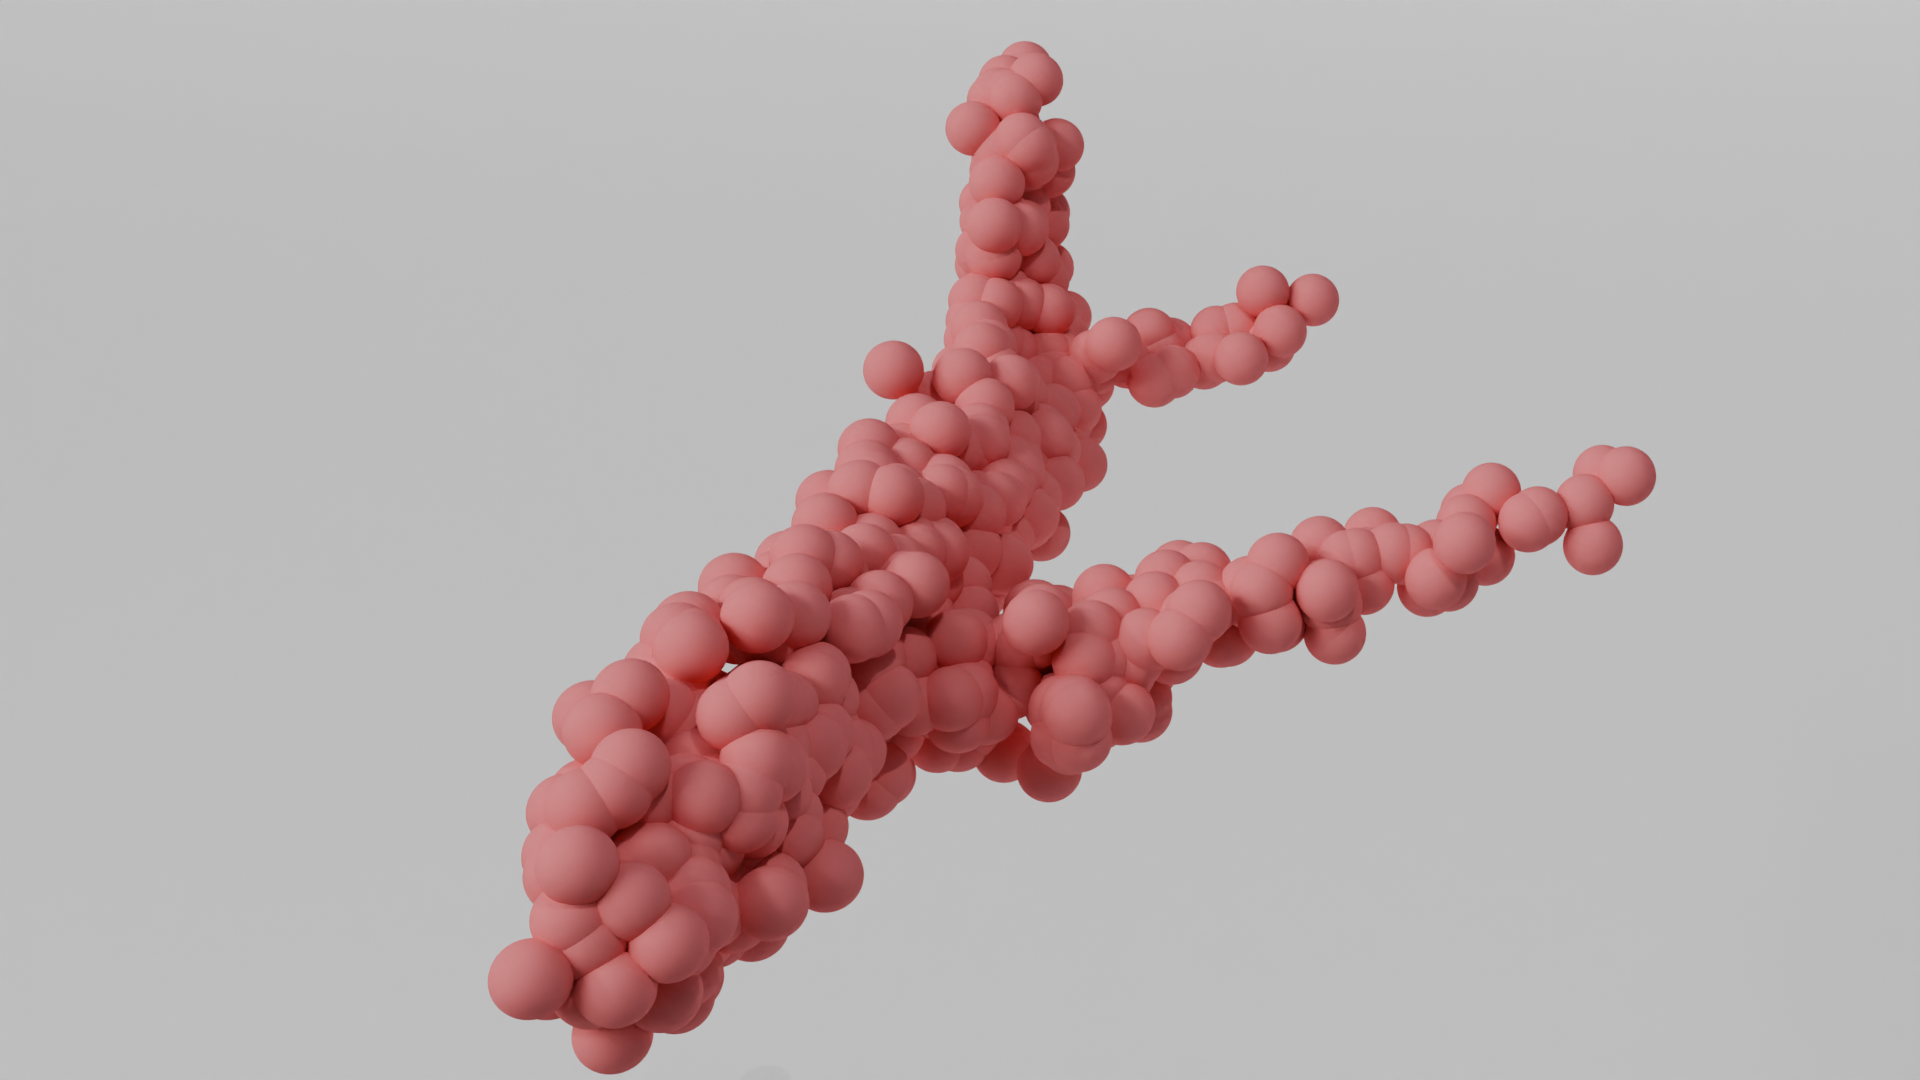
\includegraphics[width=\dimexpr\linewidth-20pt\relax]{figures/part_ap1.png}
            \makebox[20pt]{\raisebox{30pt}{\rotatebox[origin=c]{90}{\small DropCon}}}%
            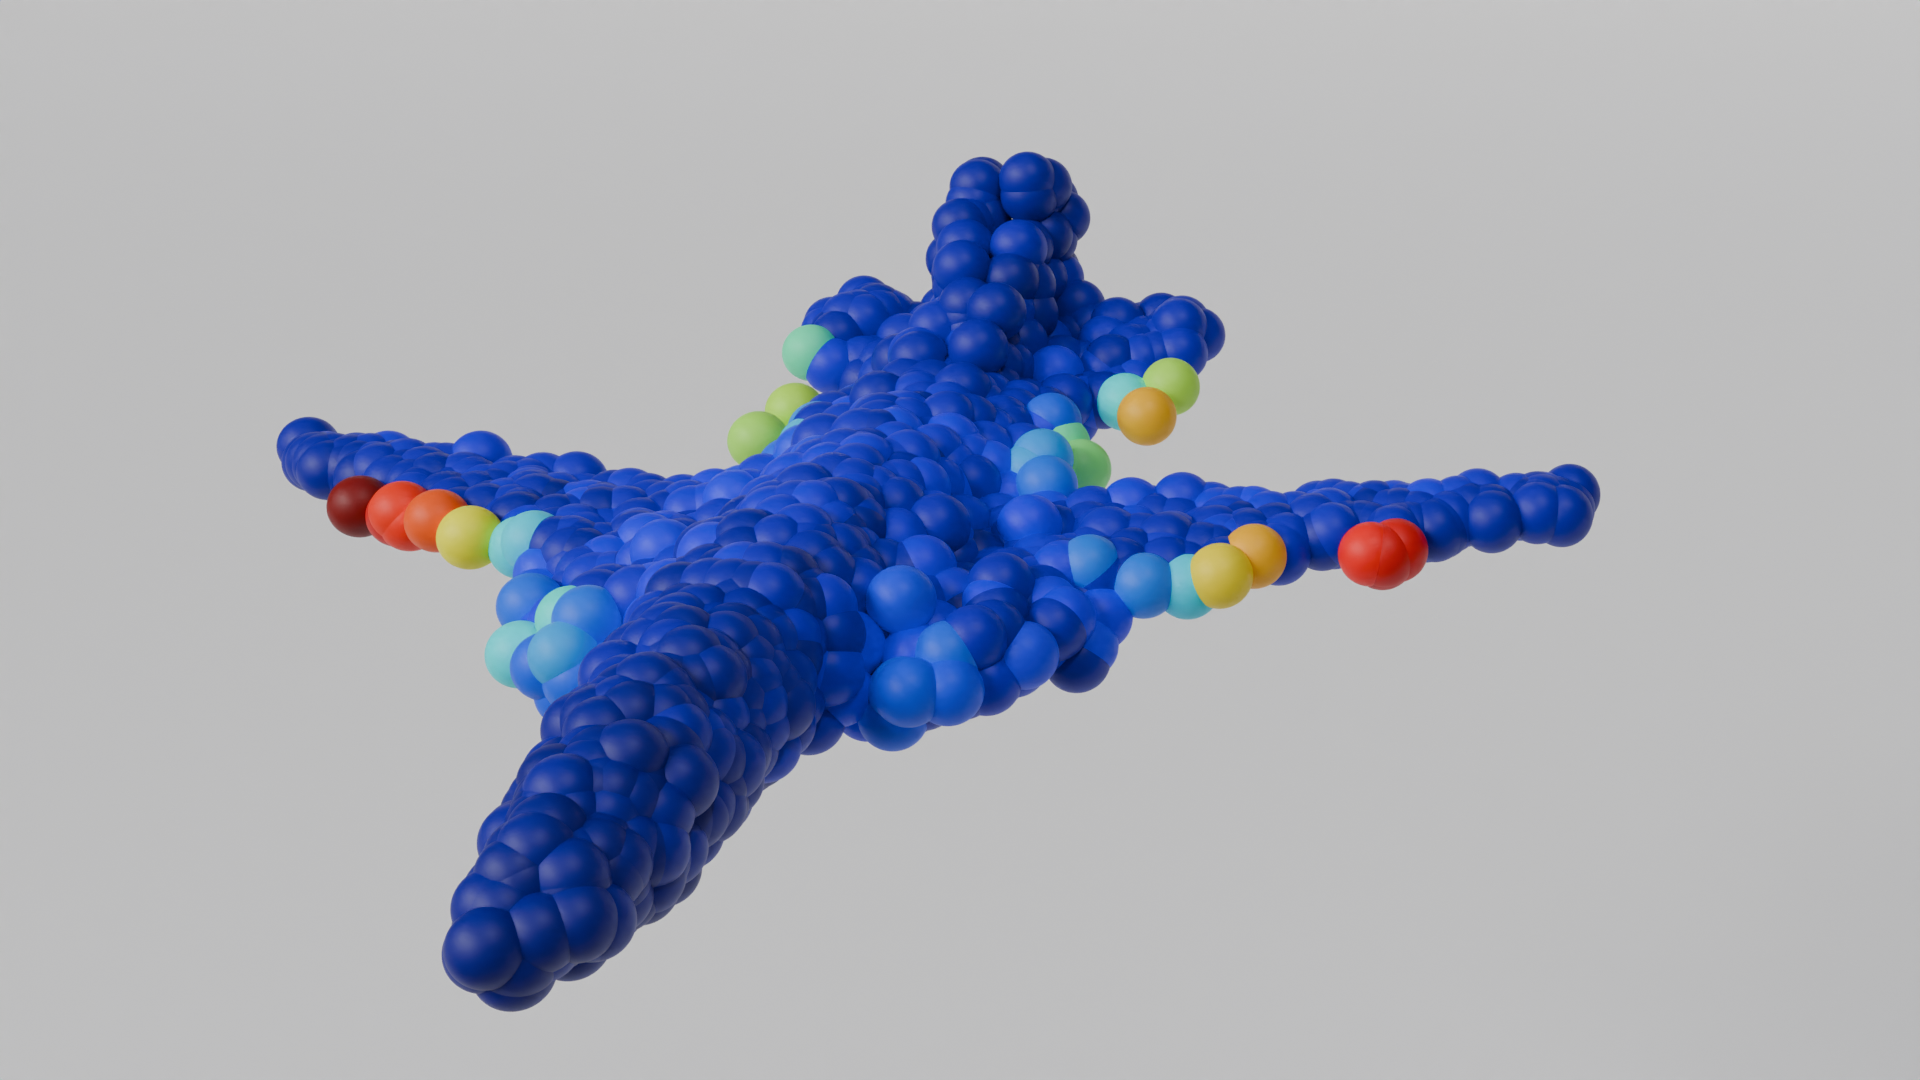
\includegraphics[width=\dimexpr\linewidth-20pt\relax]{figures/dc_lin_ap1.png}
            \makebox[20pt]{\raisebox{30pt}{\rotatebox[origin=c]{90}{\small Dropout}}}%
            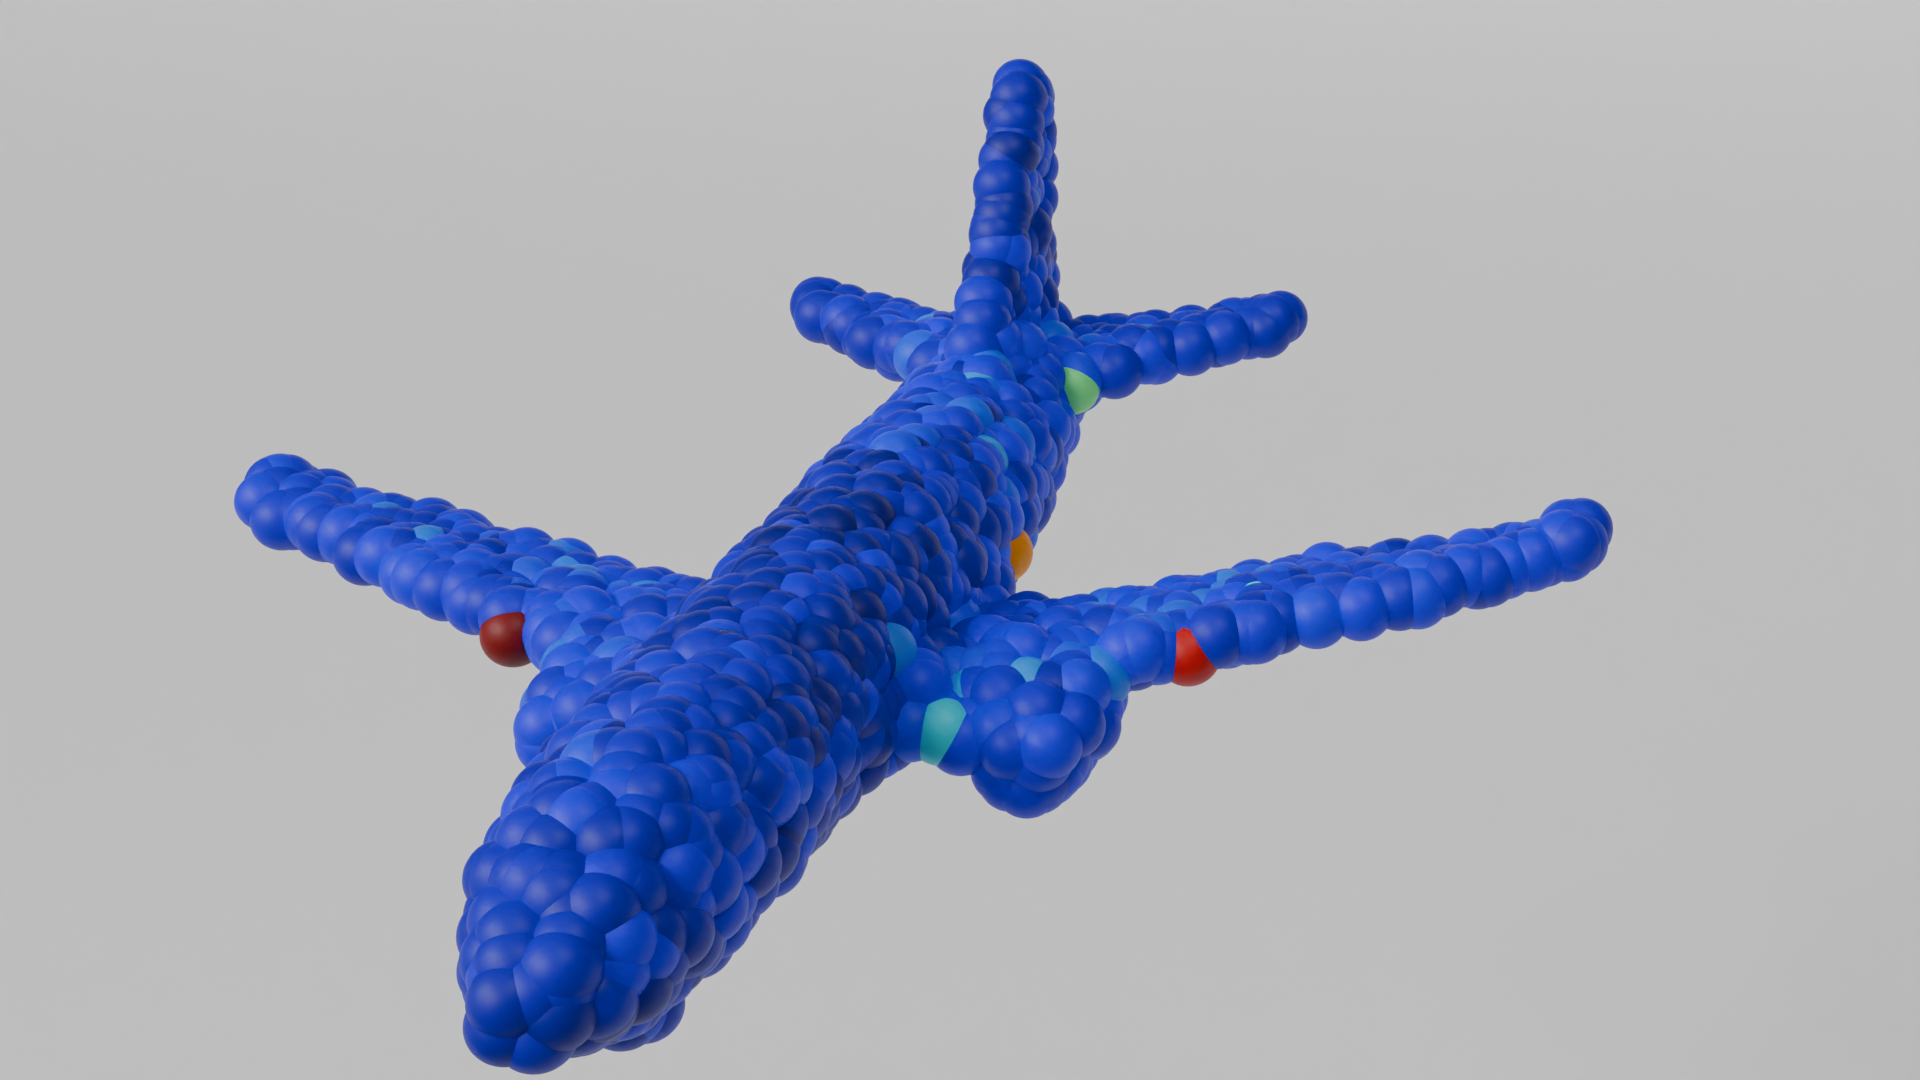
\includegraphics[width=\dimexpr\linewidth-20pt\relax]{figures/do_lin_ap1.png}
            \makebox[20pt]{\raisebox{30pt}{\rotatebox[origin=c]{90}{\small Ensemble}}}%
            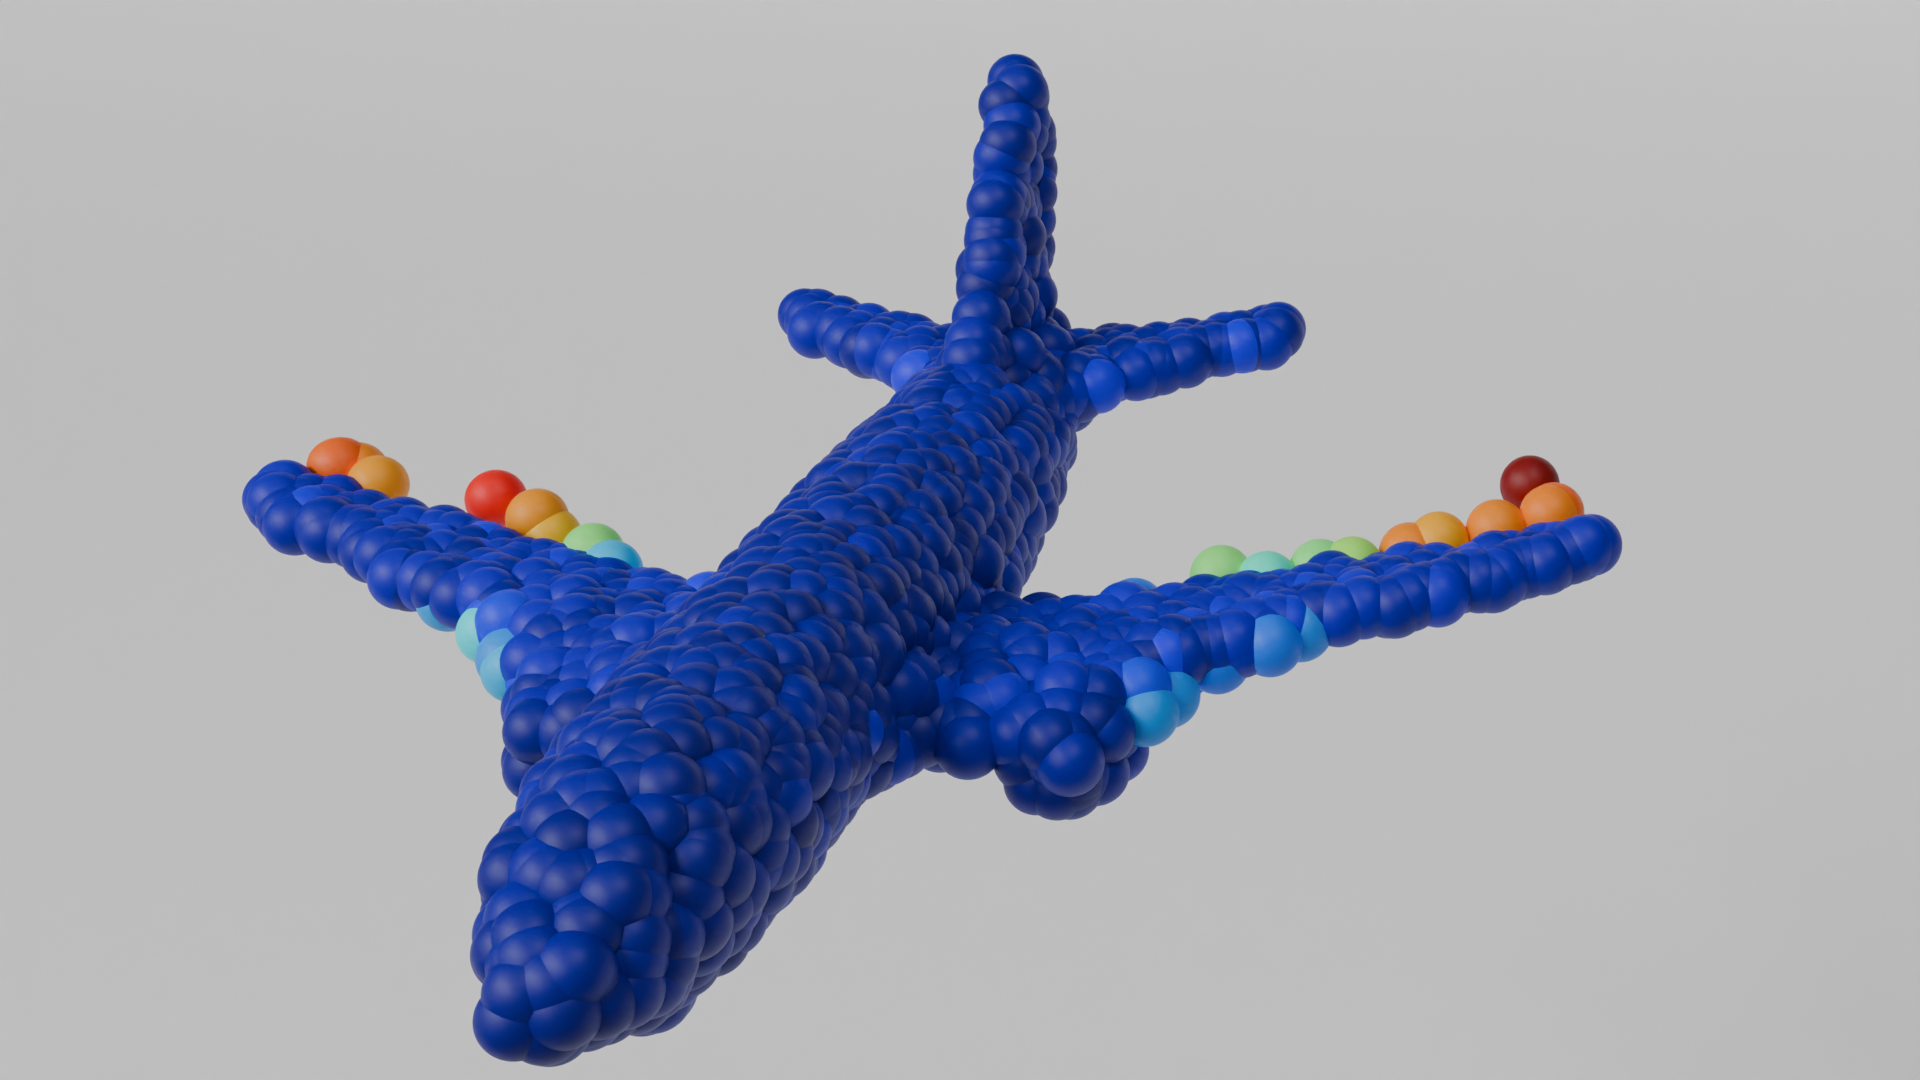
\includegraphics[width=\dimexpr\linewidth-20pt\relax]{figures/ens_lin_ap1.png}
            \makebox[20pt]{\raisebox{30pt}{\rotatebox[origin=c]{90}{\small Implicit}}}%
            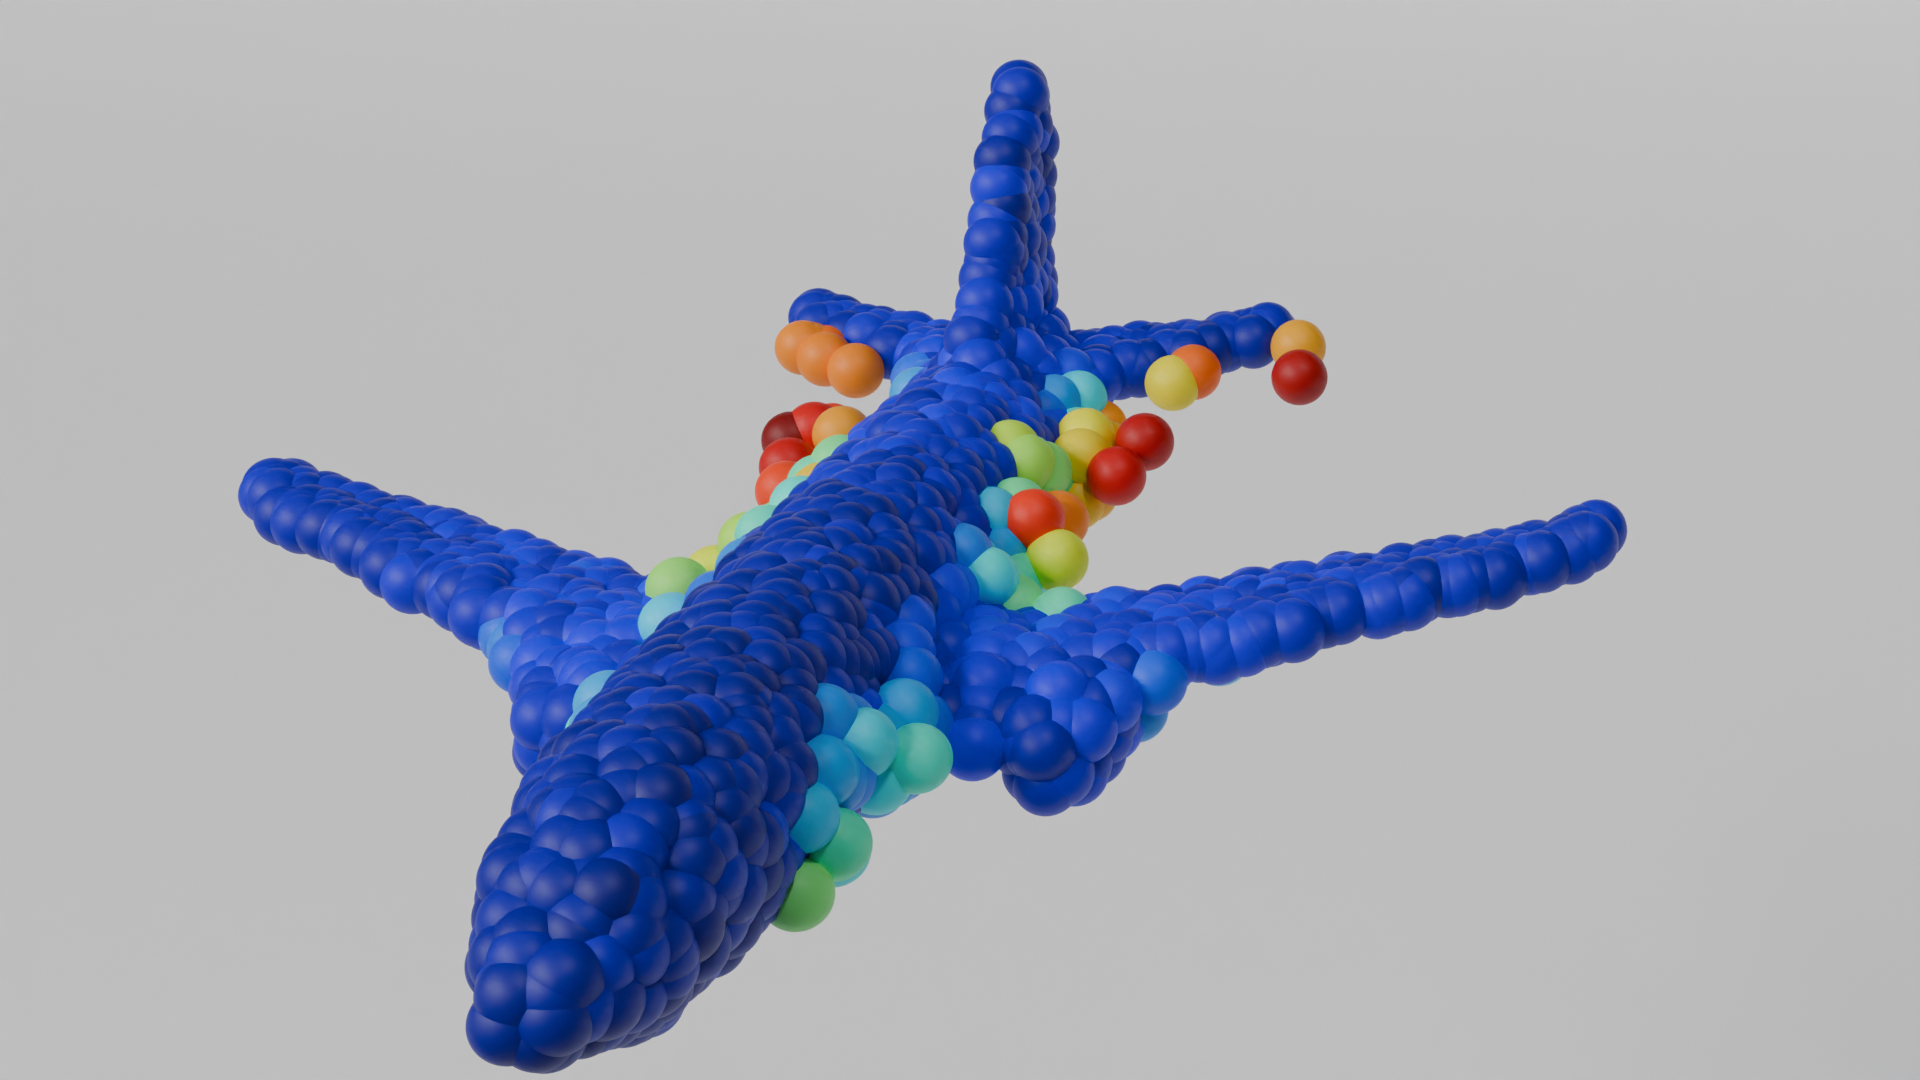
\includegraphics[width=\dimexpr\linewidth-20pt\relax]{figures/iml_lin_ap1.png}
            \makebox[20pt]{\raisebox{30pt}{\rotatebox[origin=c]{90}{\small GT}}}%
            \includegraphics[width=\dimexpr\linewidth-20pt\relax]{figures/com_ap1.png}
            \caption{Airplane 1}
          \end{subfigure}\hfill
          \begin{subfigure}[t]{0.315\textwidth}
            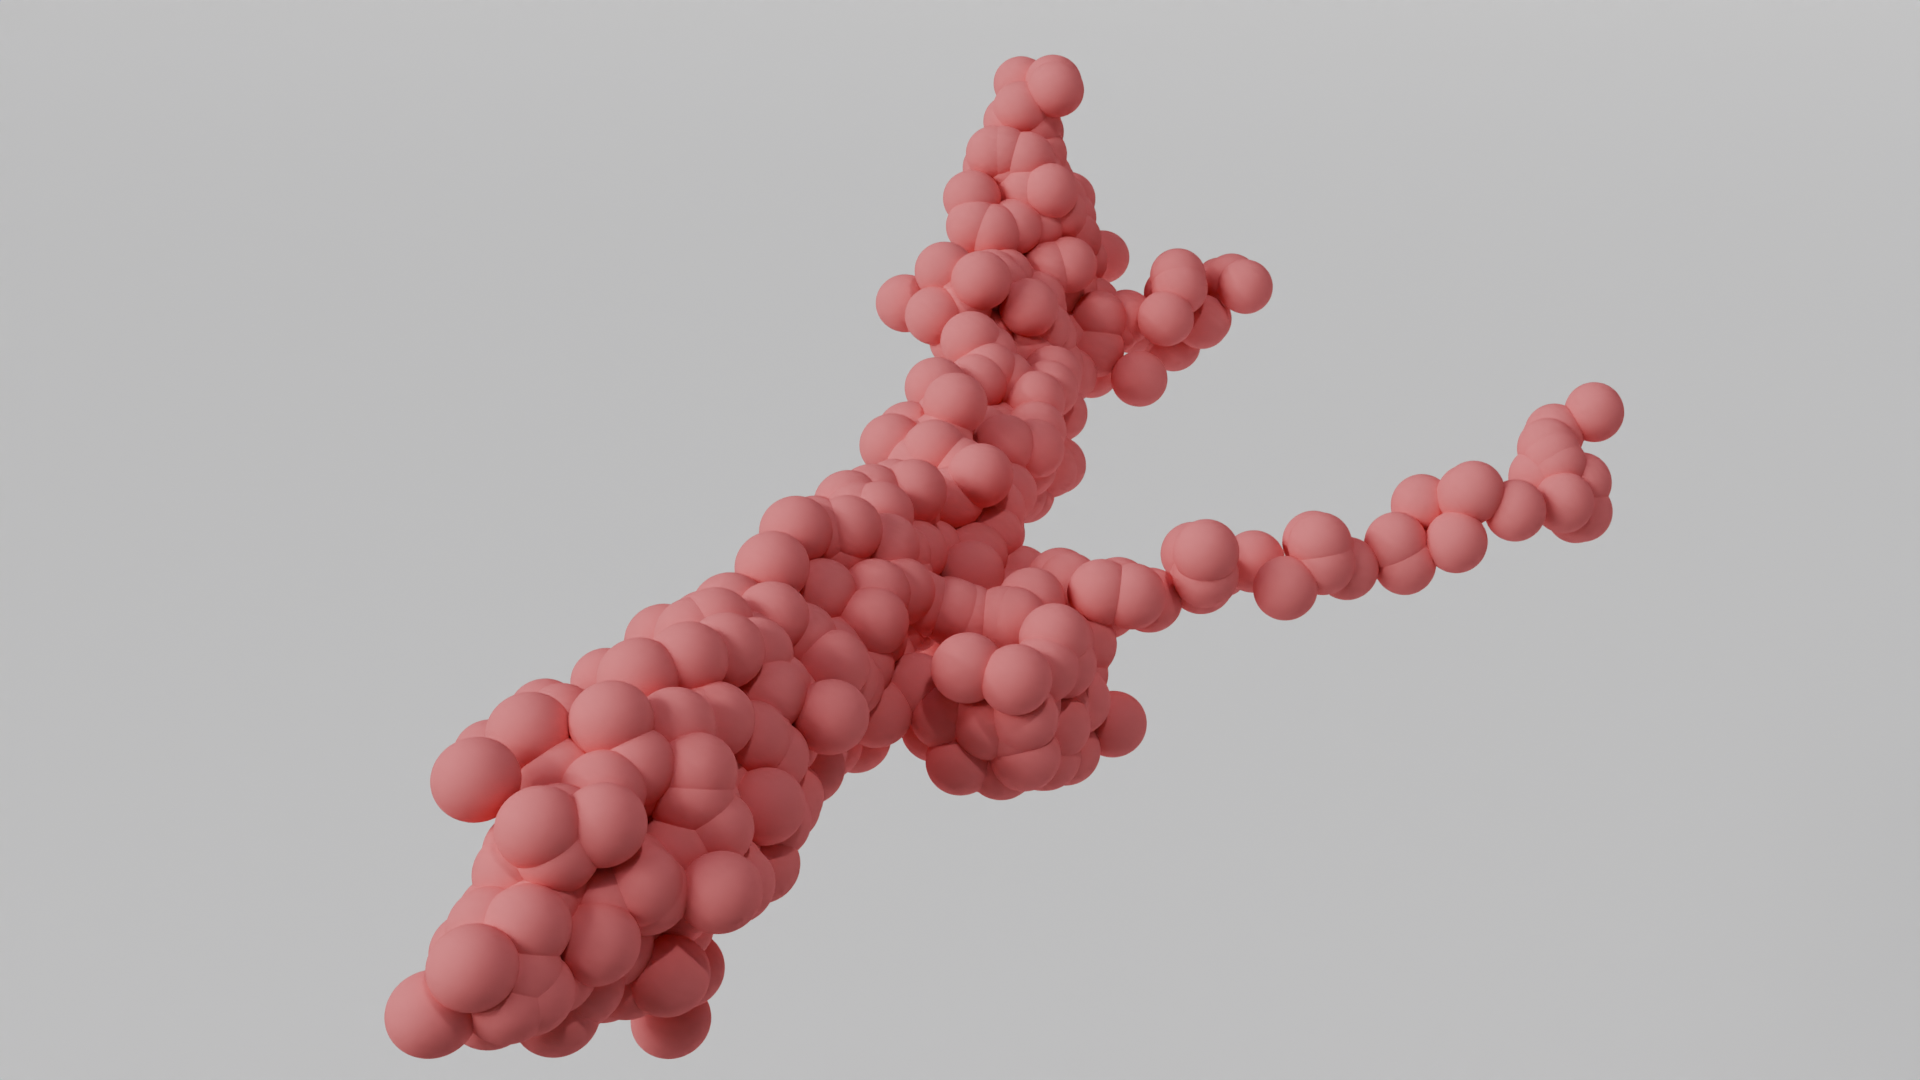
\includegraphics[width=\textwidth]{figures/part_ap2.png}
            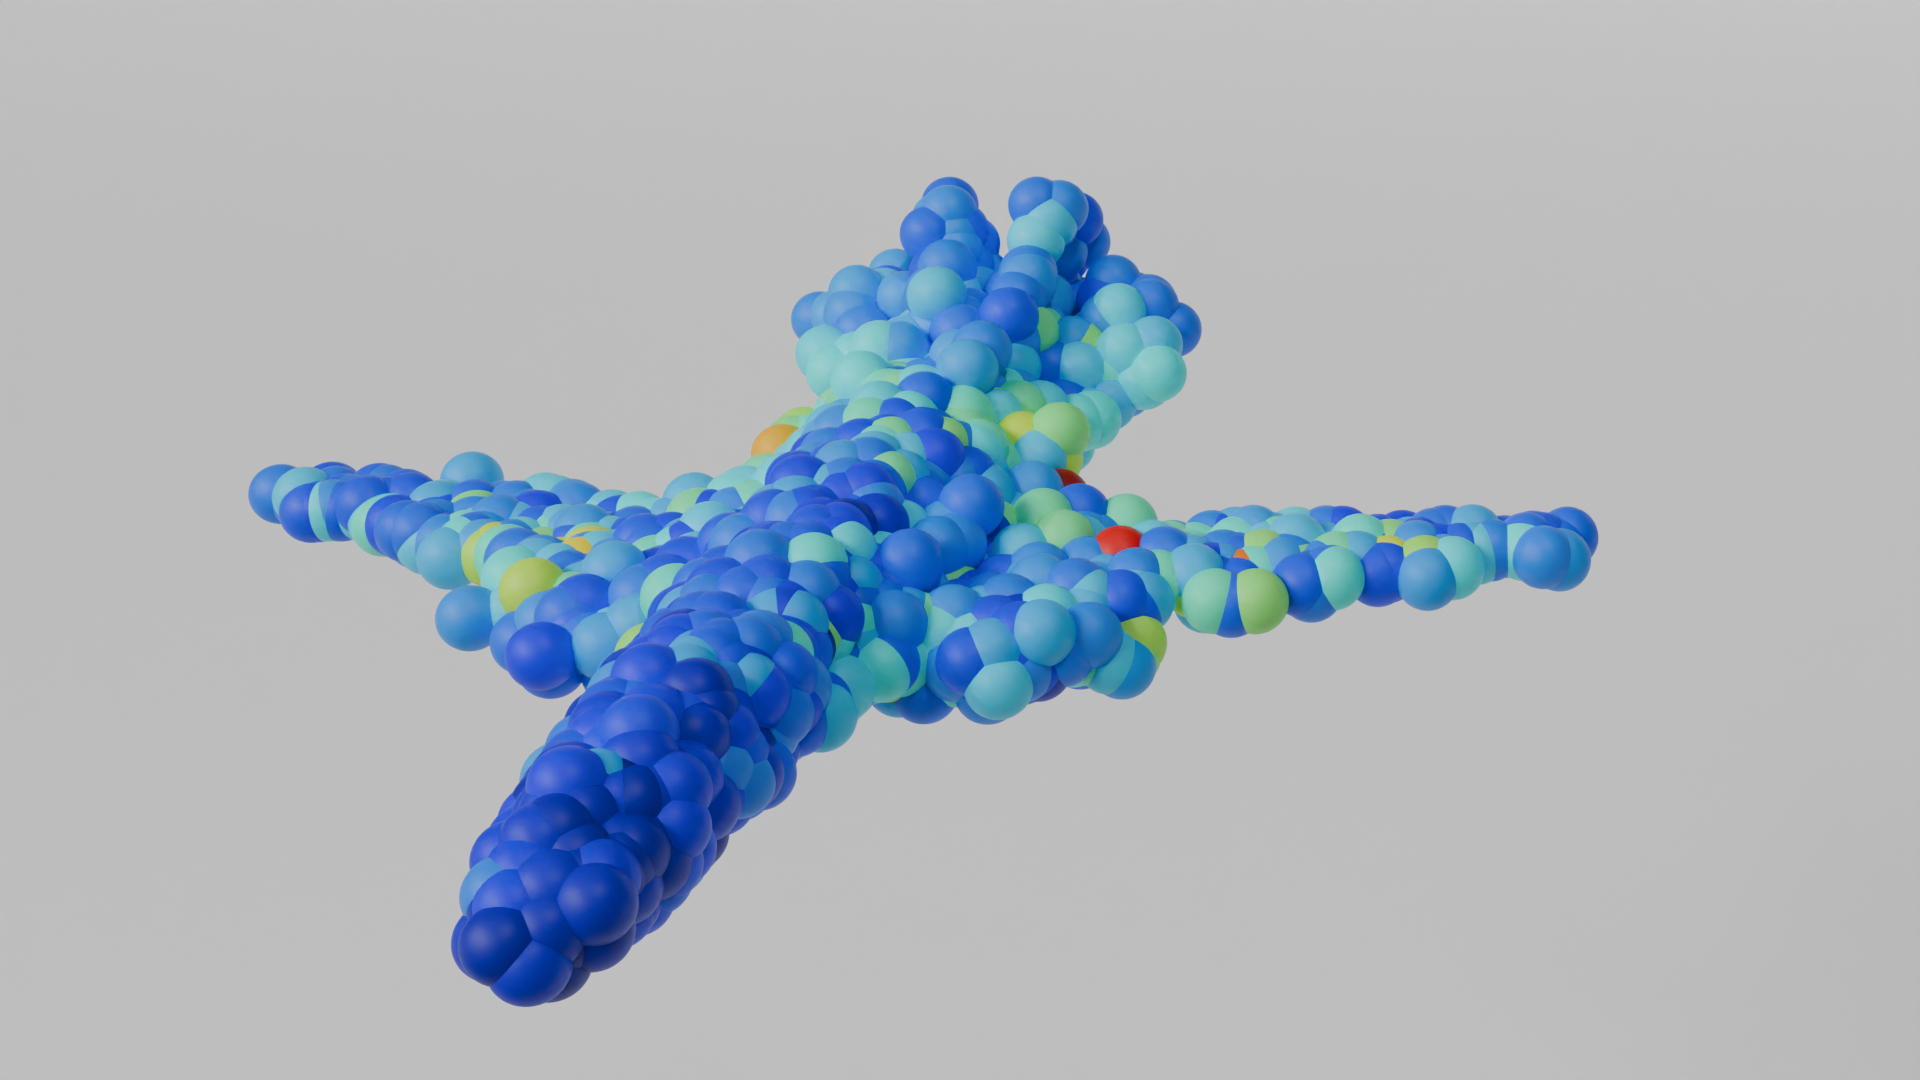
\includegraphics[width=\textwidth]{figures/dc_lin_ap2.png}
            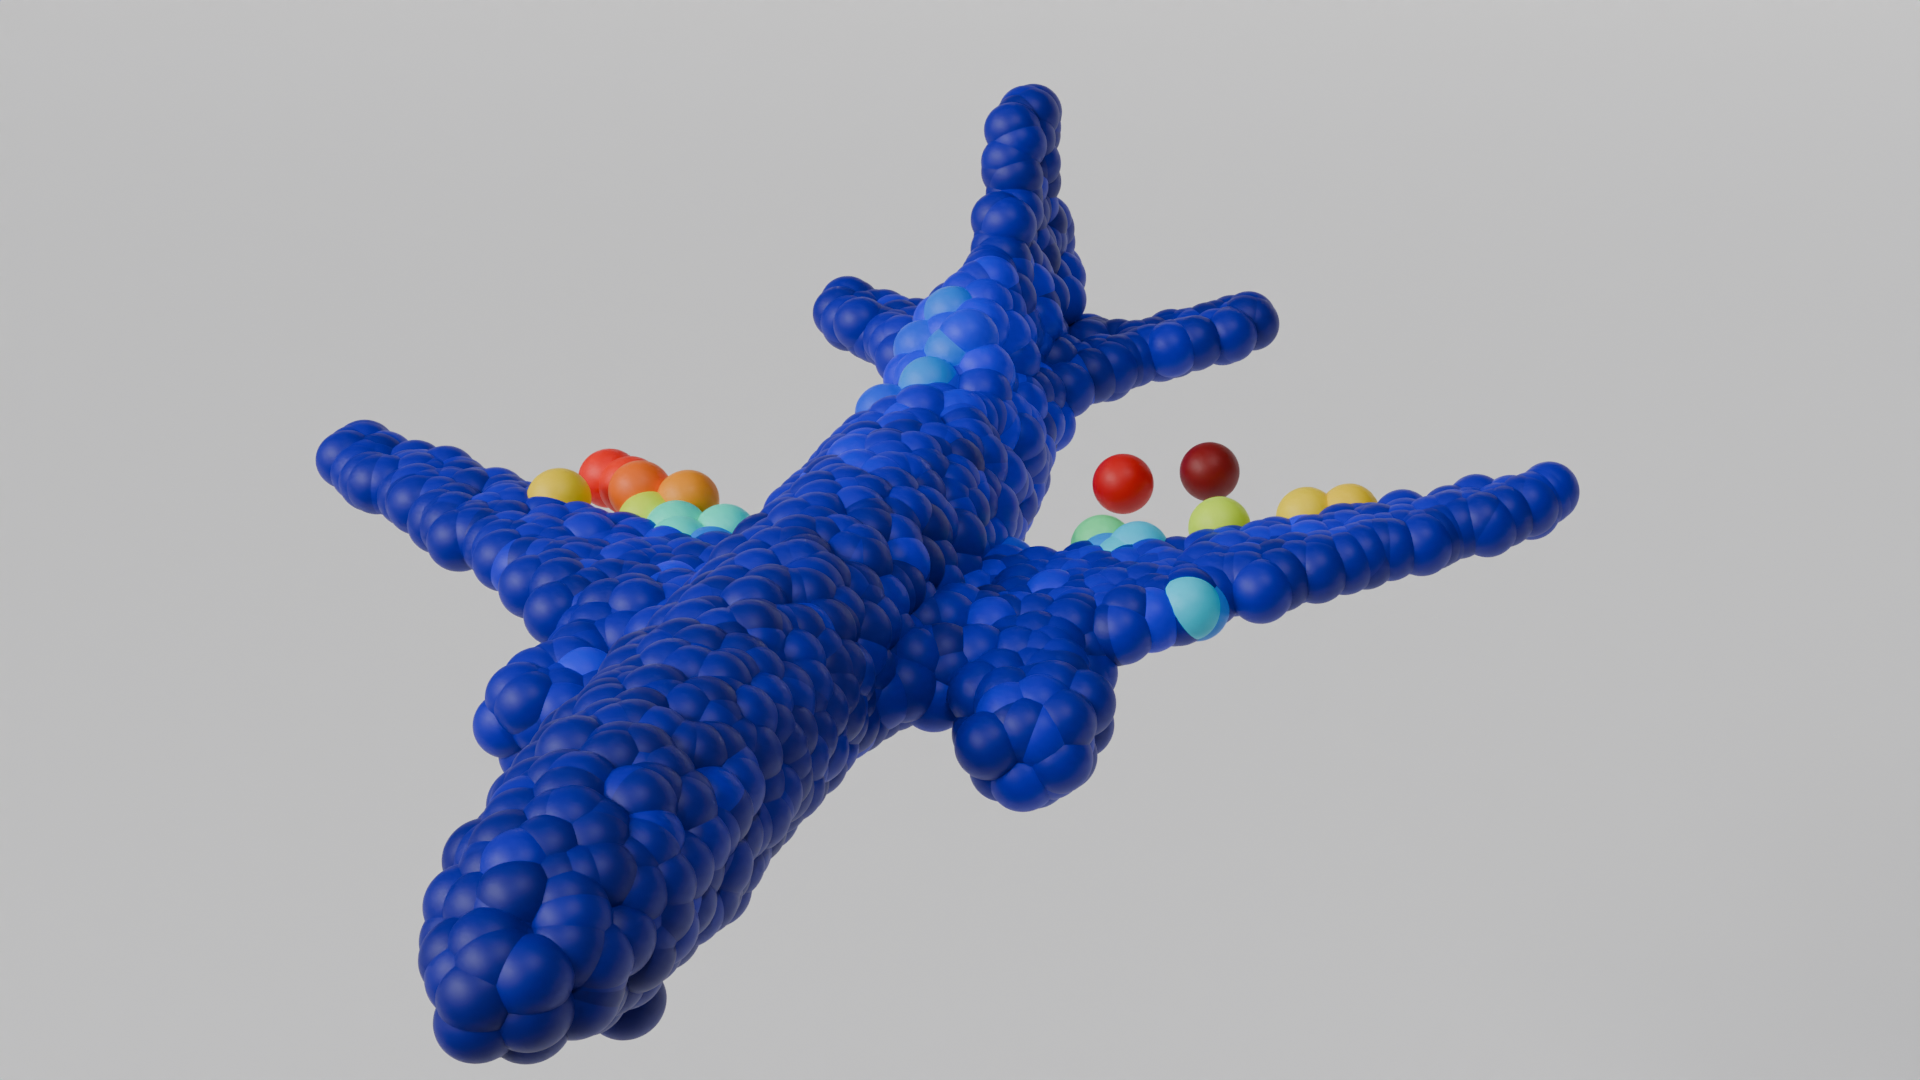
\includegraphics[width=\textwidth]{figures/do_lin_ap2.png}
            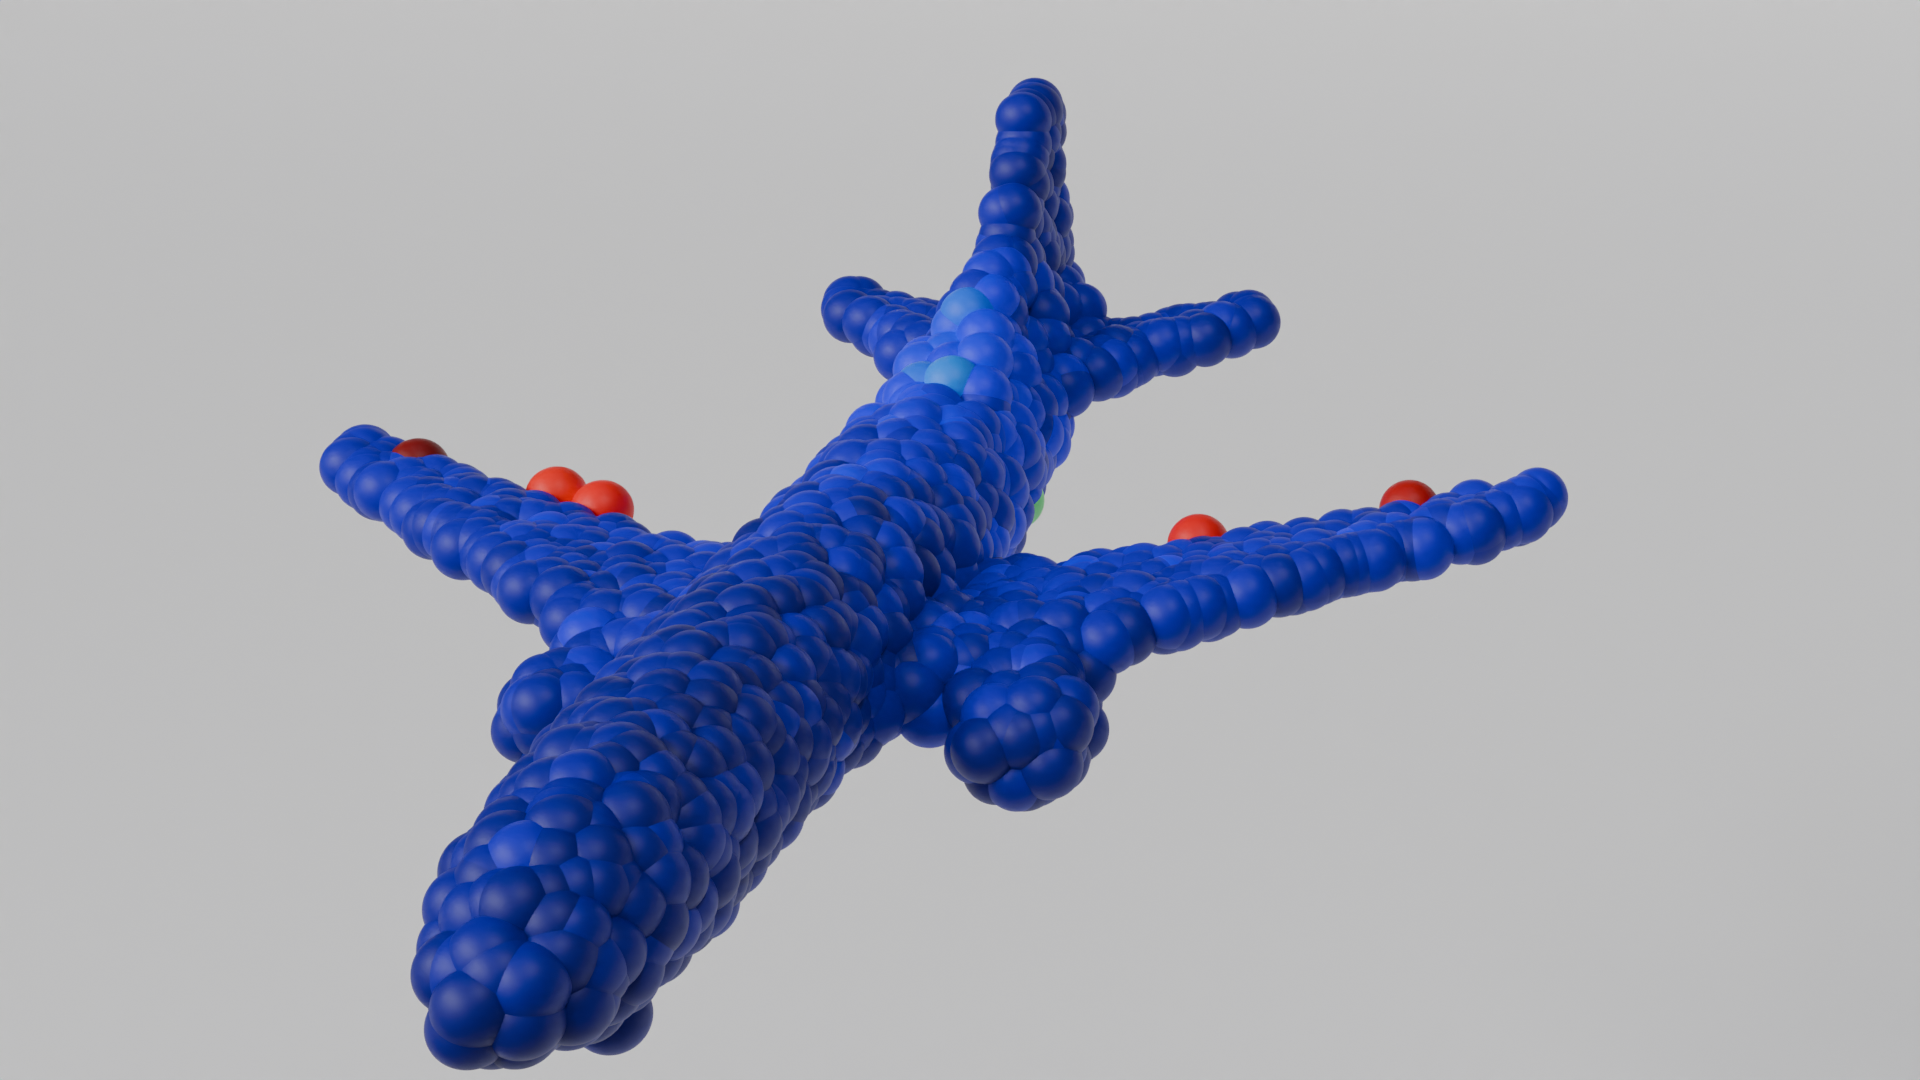
\includegraphics[width=\textwidth]{figures/ens_lin_ap2.png}
            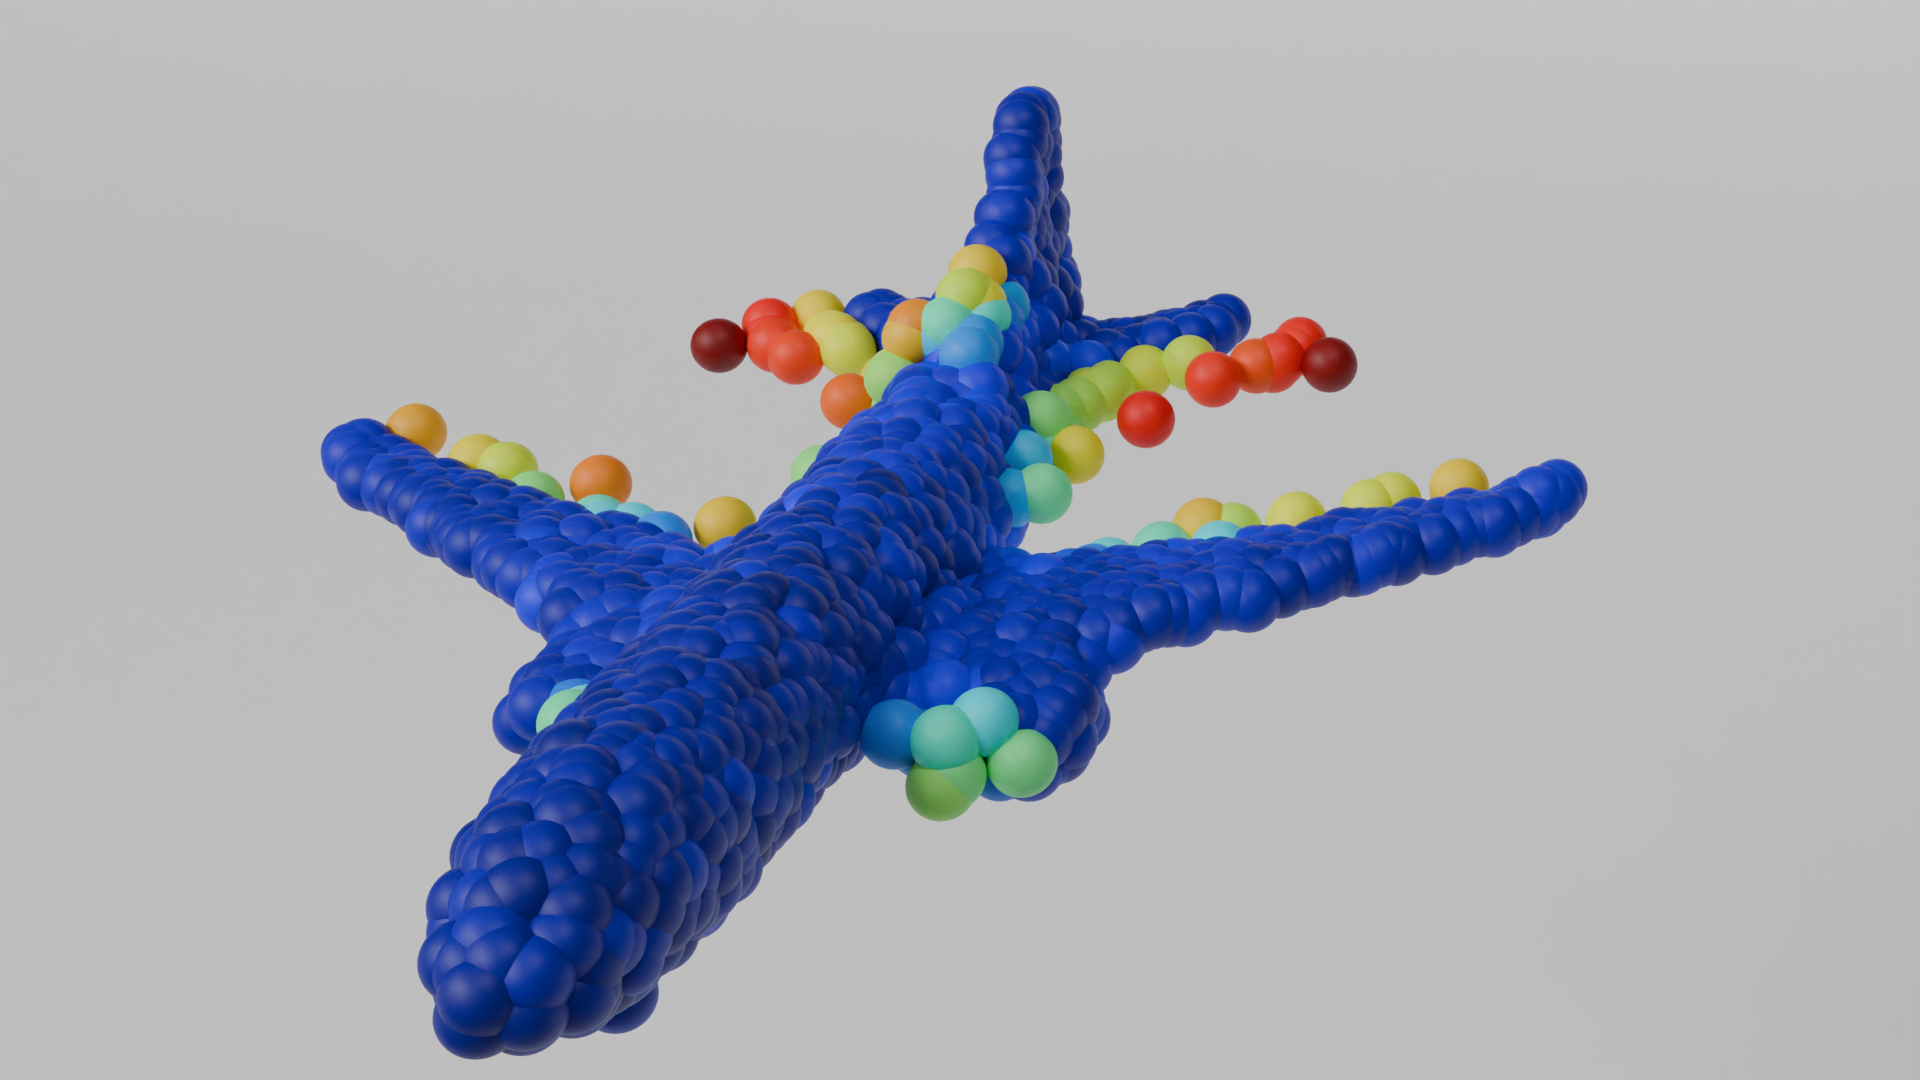
\includegraphics[width=\textwidth]{figures/iml_lin_ap2.png}
            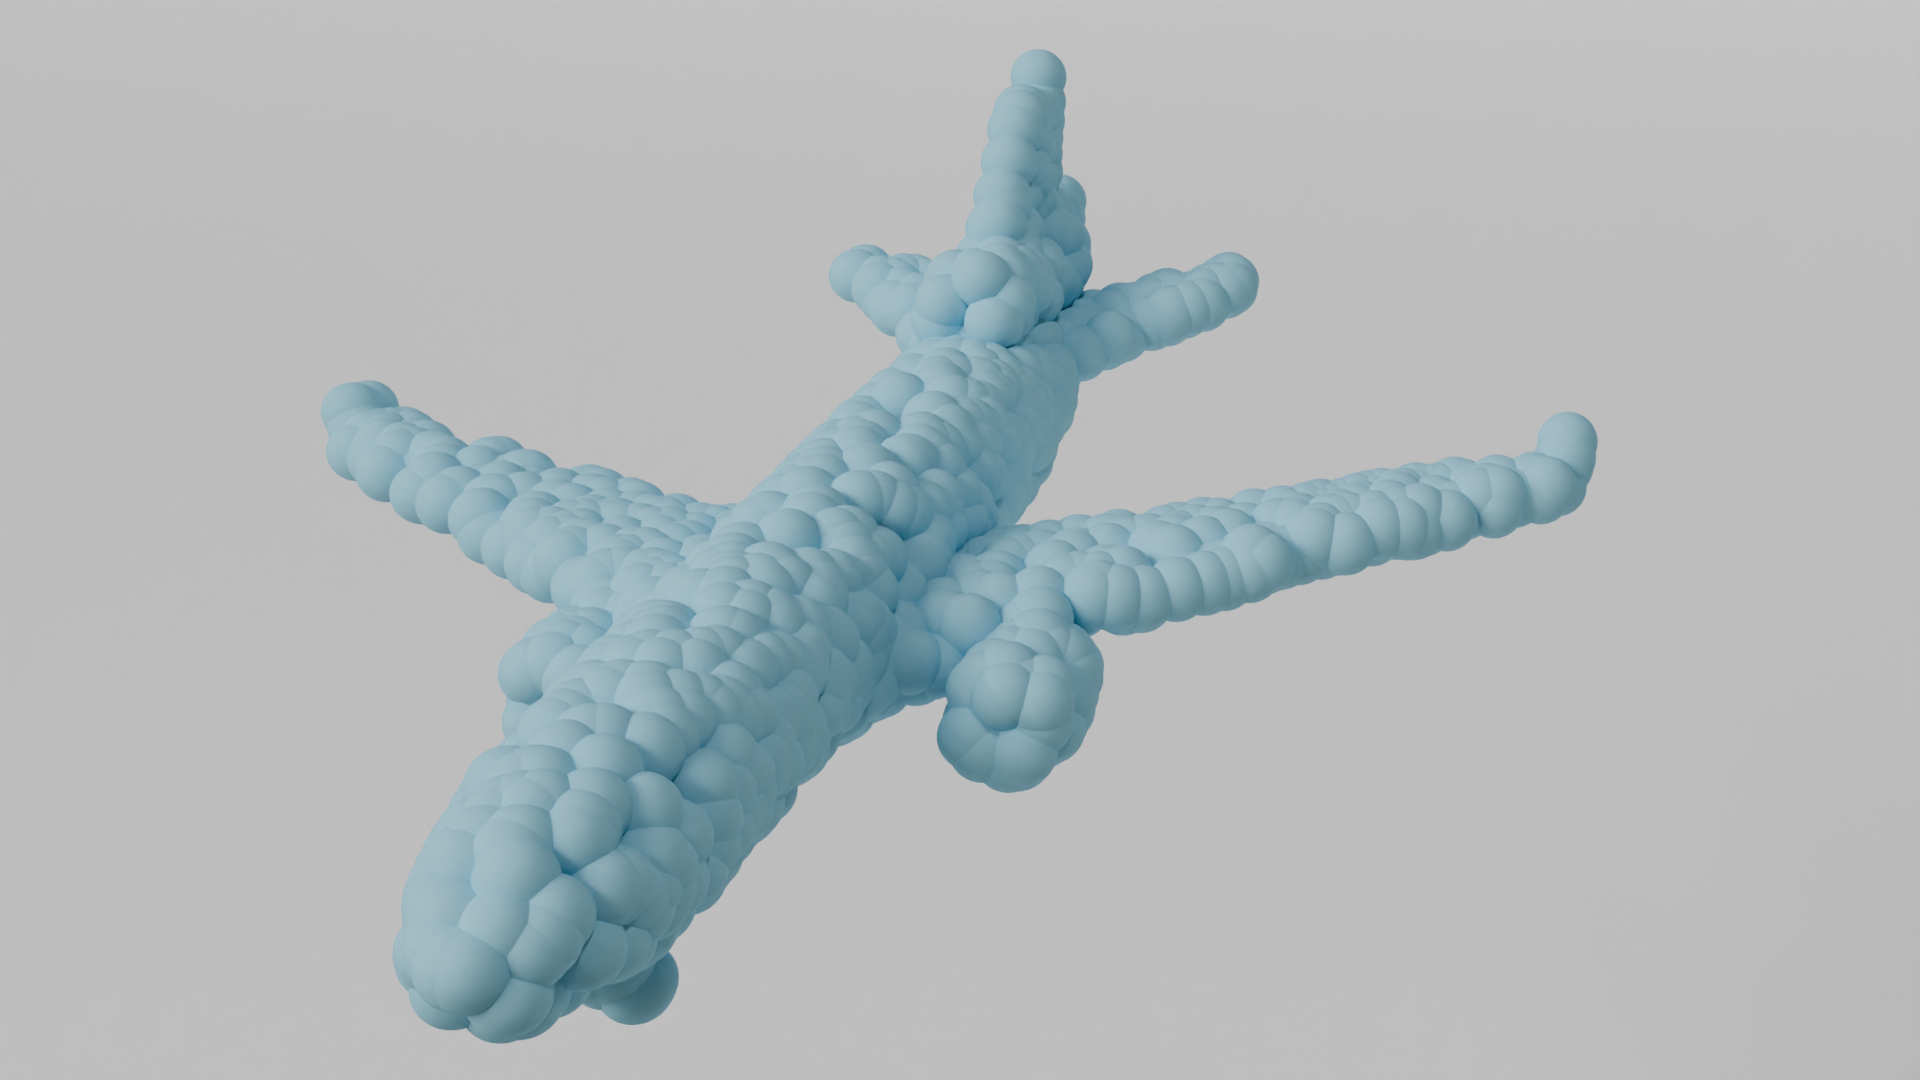
\includegraphics[width=\textwidth]{figures/com_ap2.png}
            \caption{Airplane 2}
          \end{subfigure}\hfill
          \begin{subfigure}[t]{0.315\textwidth}
            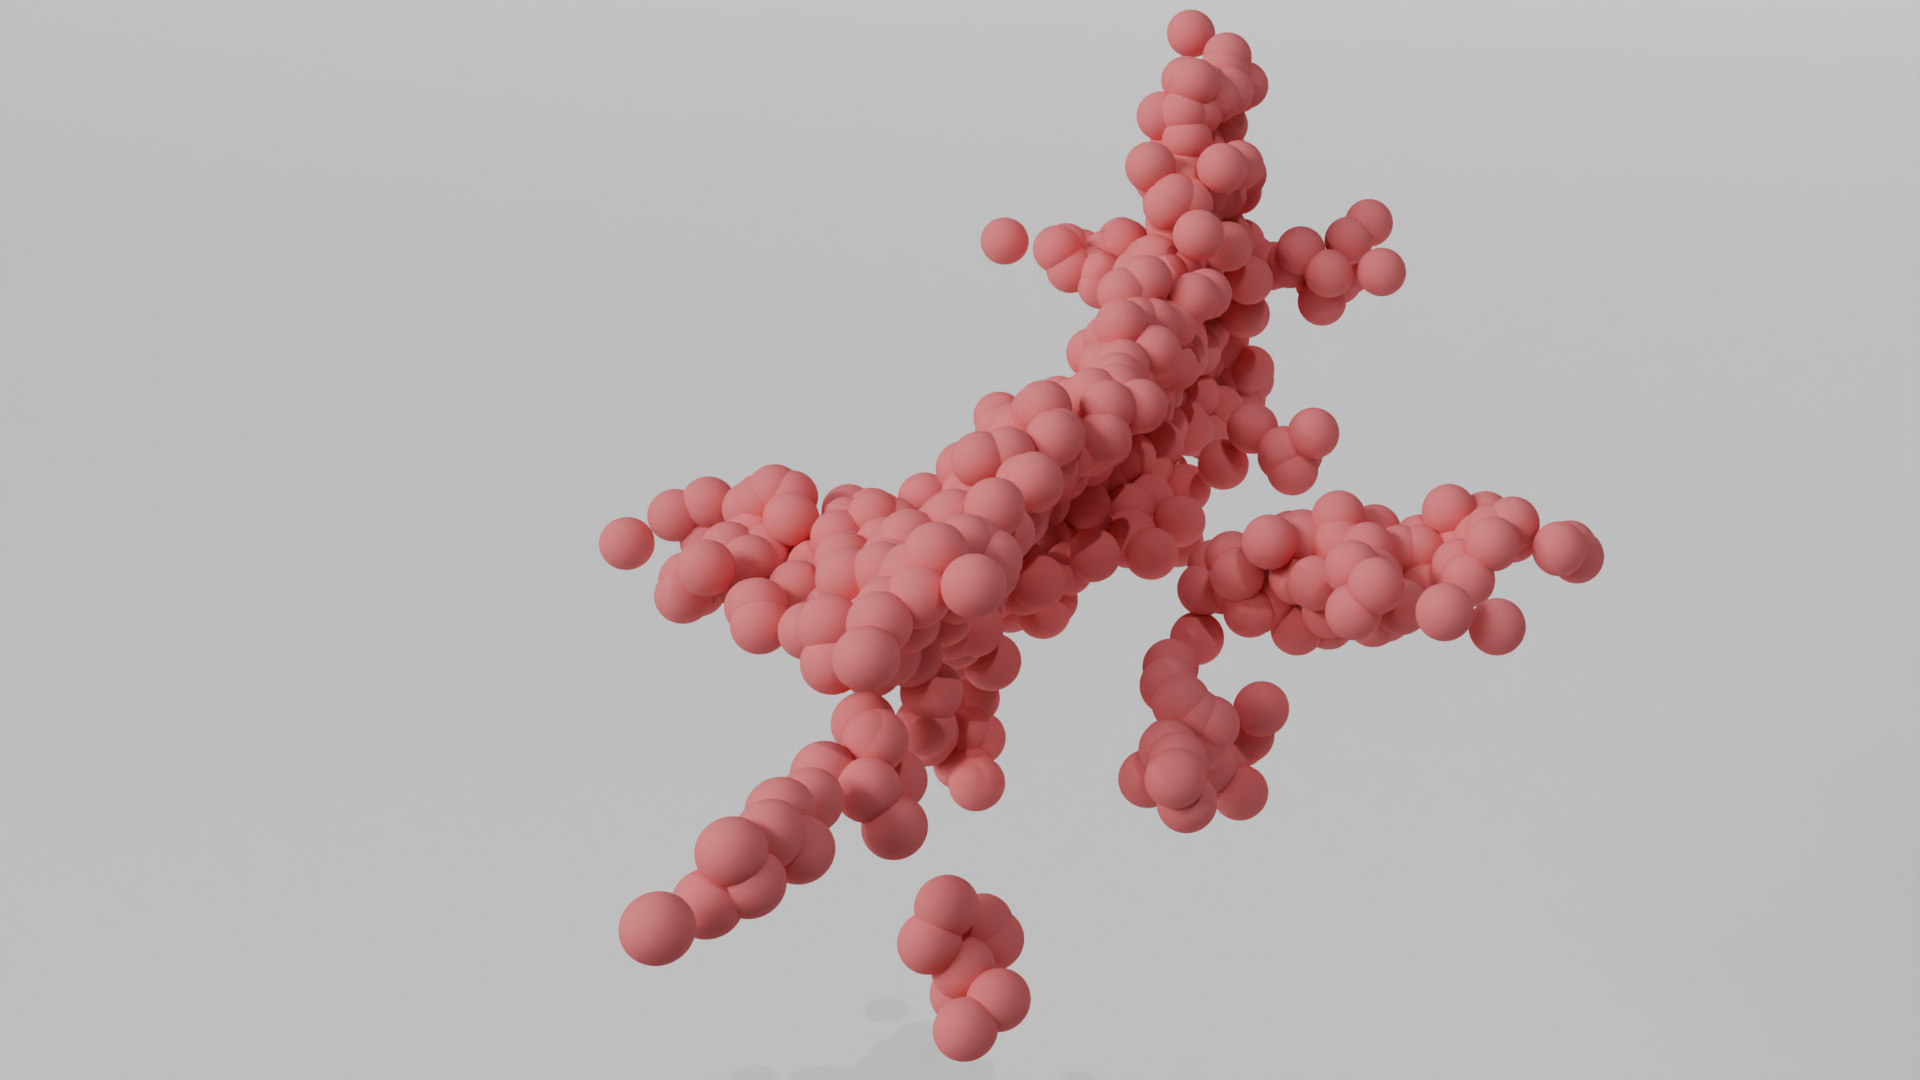
\includegraphics[width=\textwidth]{figures/part_ap3.png}
            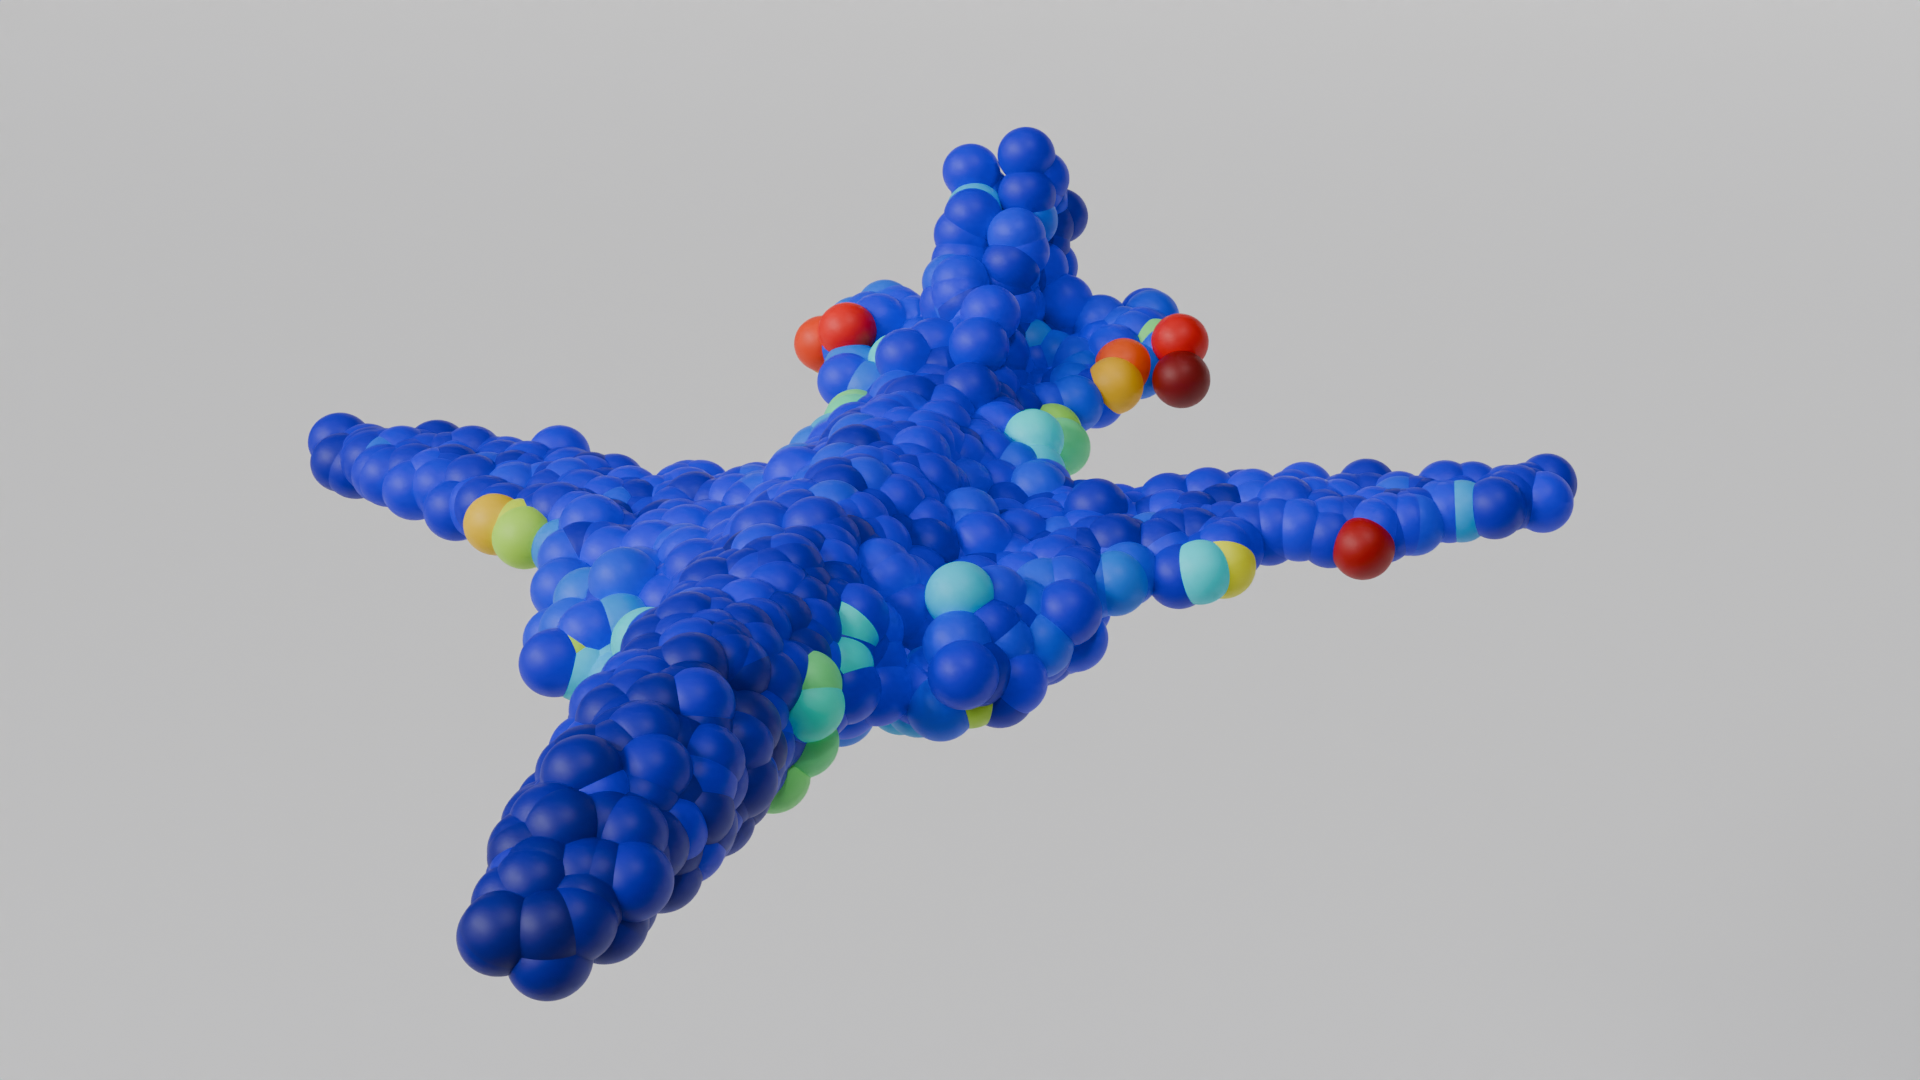
\includegraphics[width=\textwidth]{figures/dc_lin_ap3.png}
            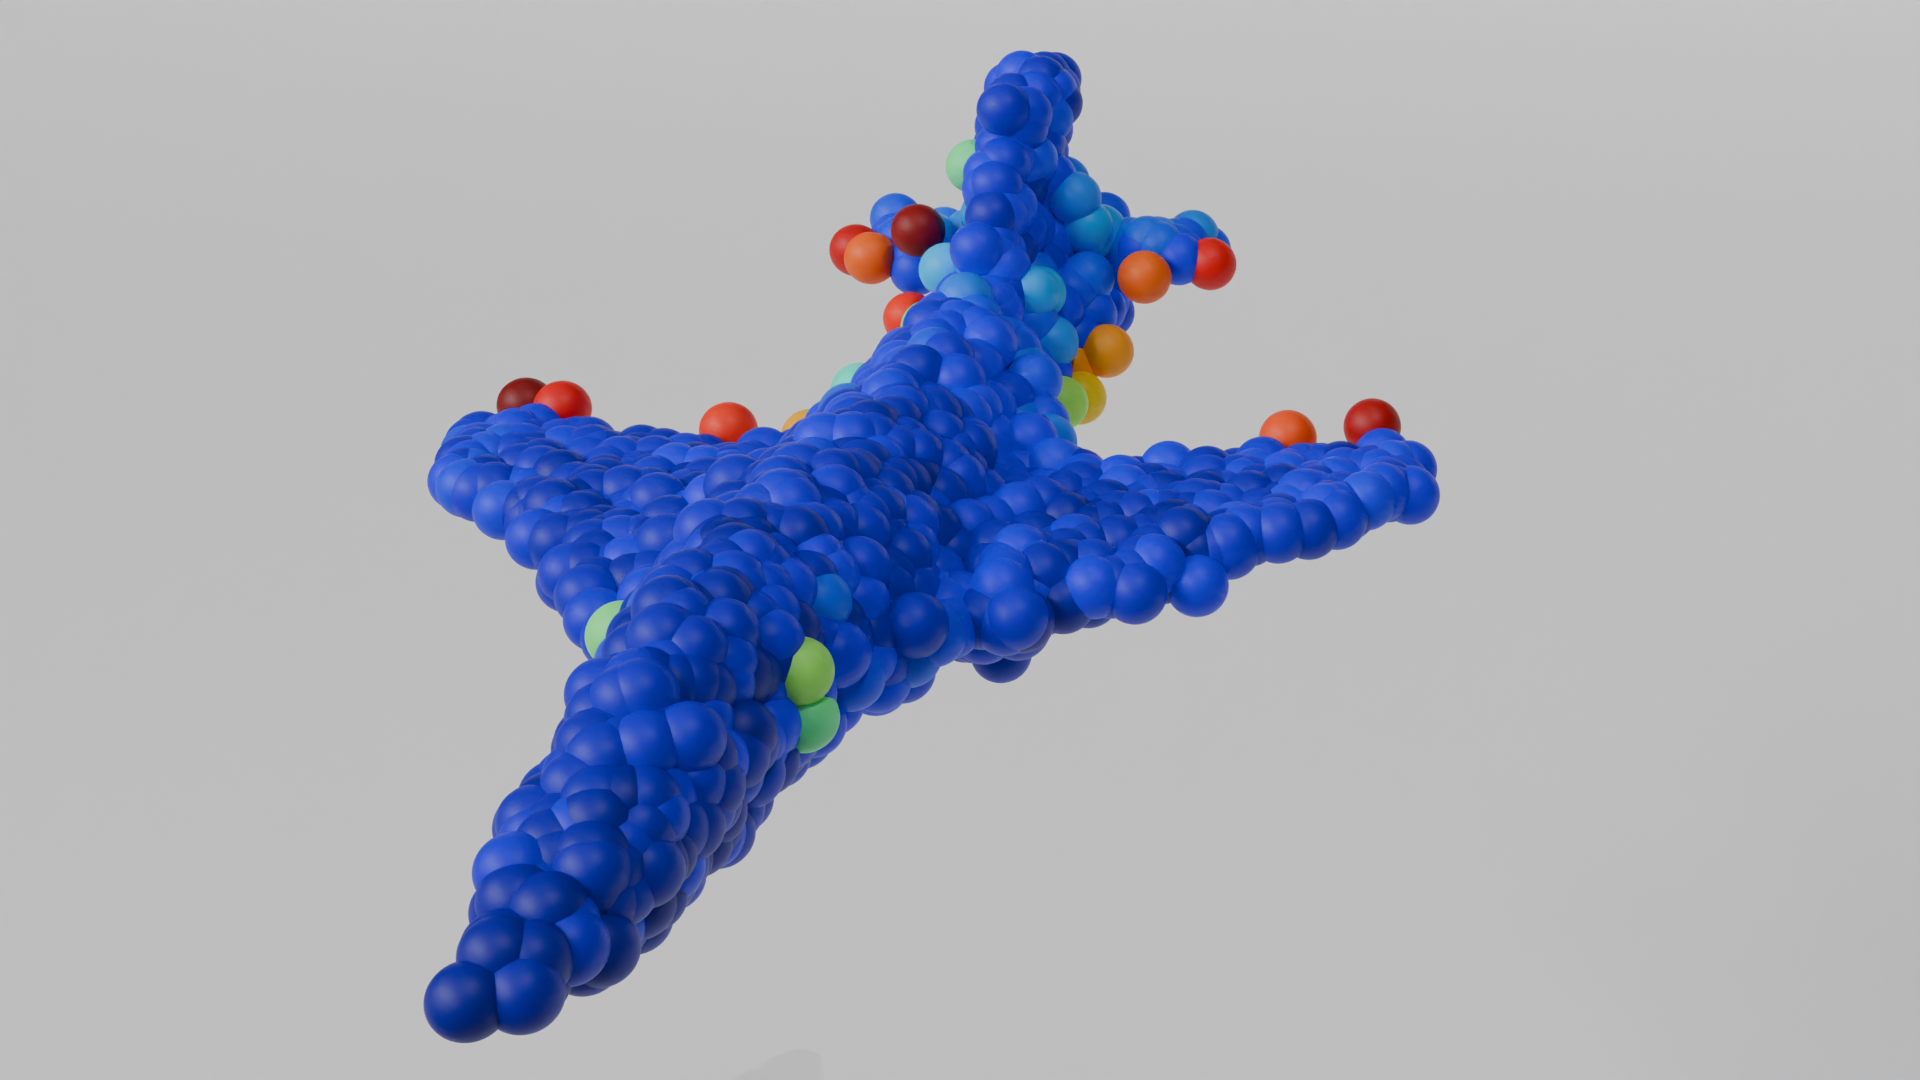
\includegraphics[width=\textwidth]{figures/do_lin_ap3.png}
            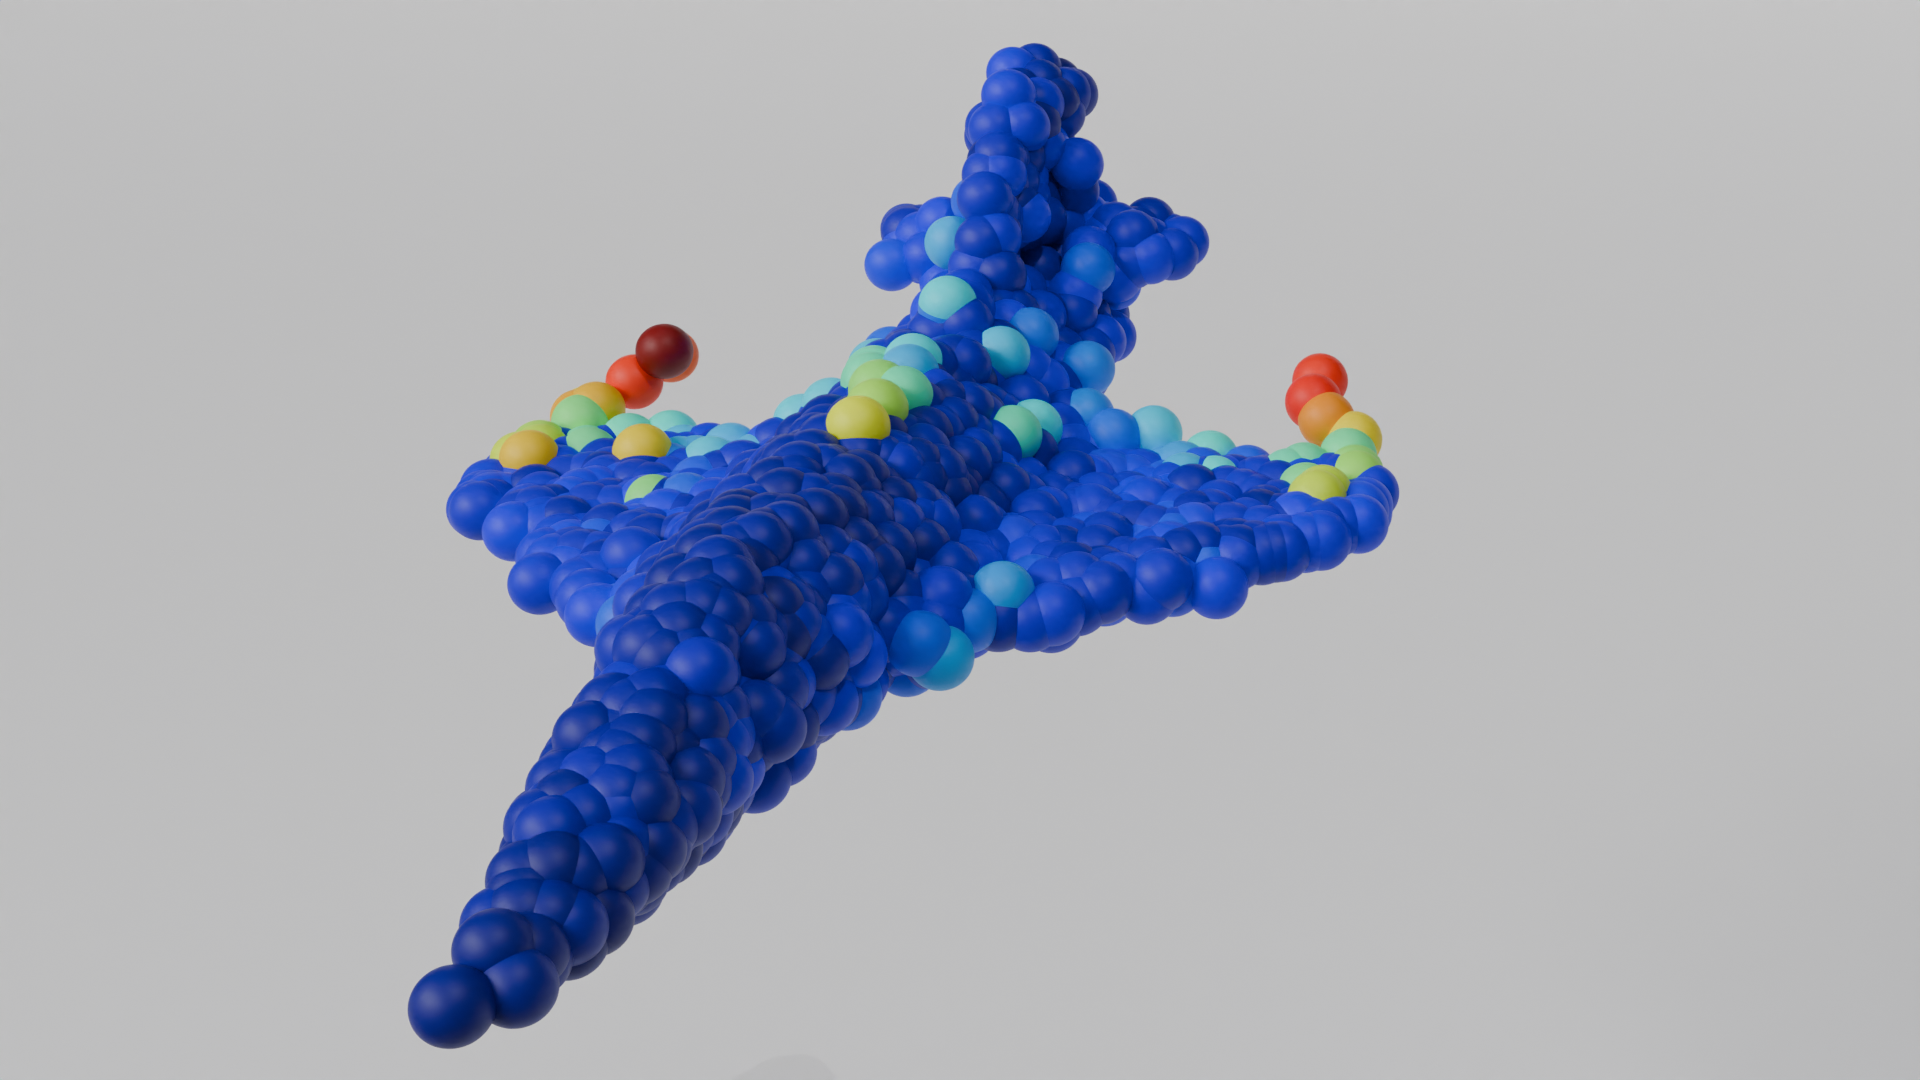
\includegraphics[width=\textwidth]{figures/ens_lin_ap3.png}
            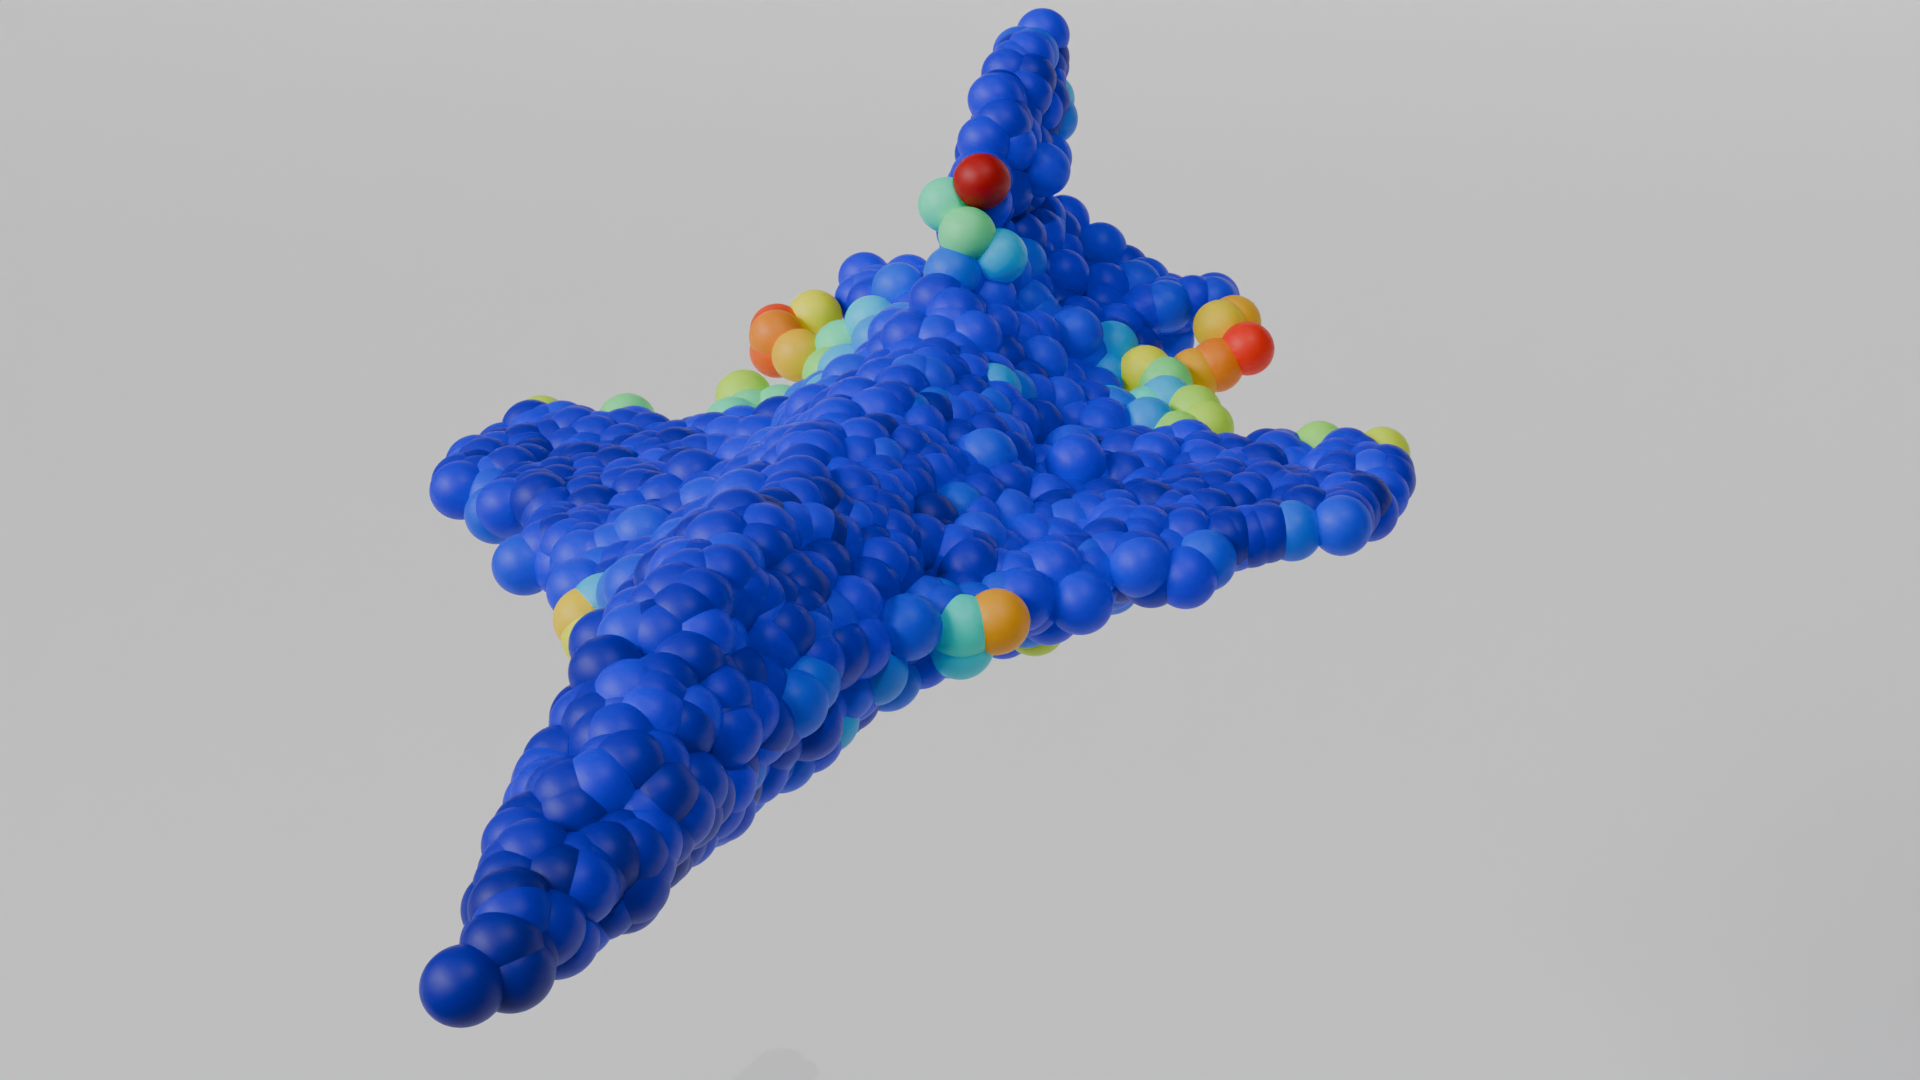
\includegraphics[width=\textwidth]{figures/iml_lin_ap3.png}
            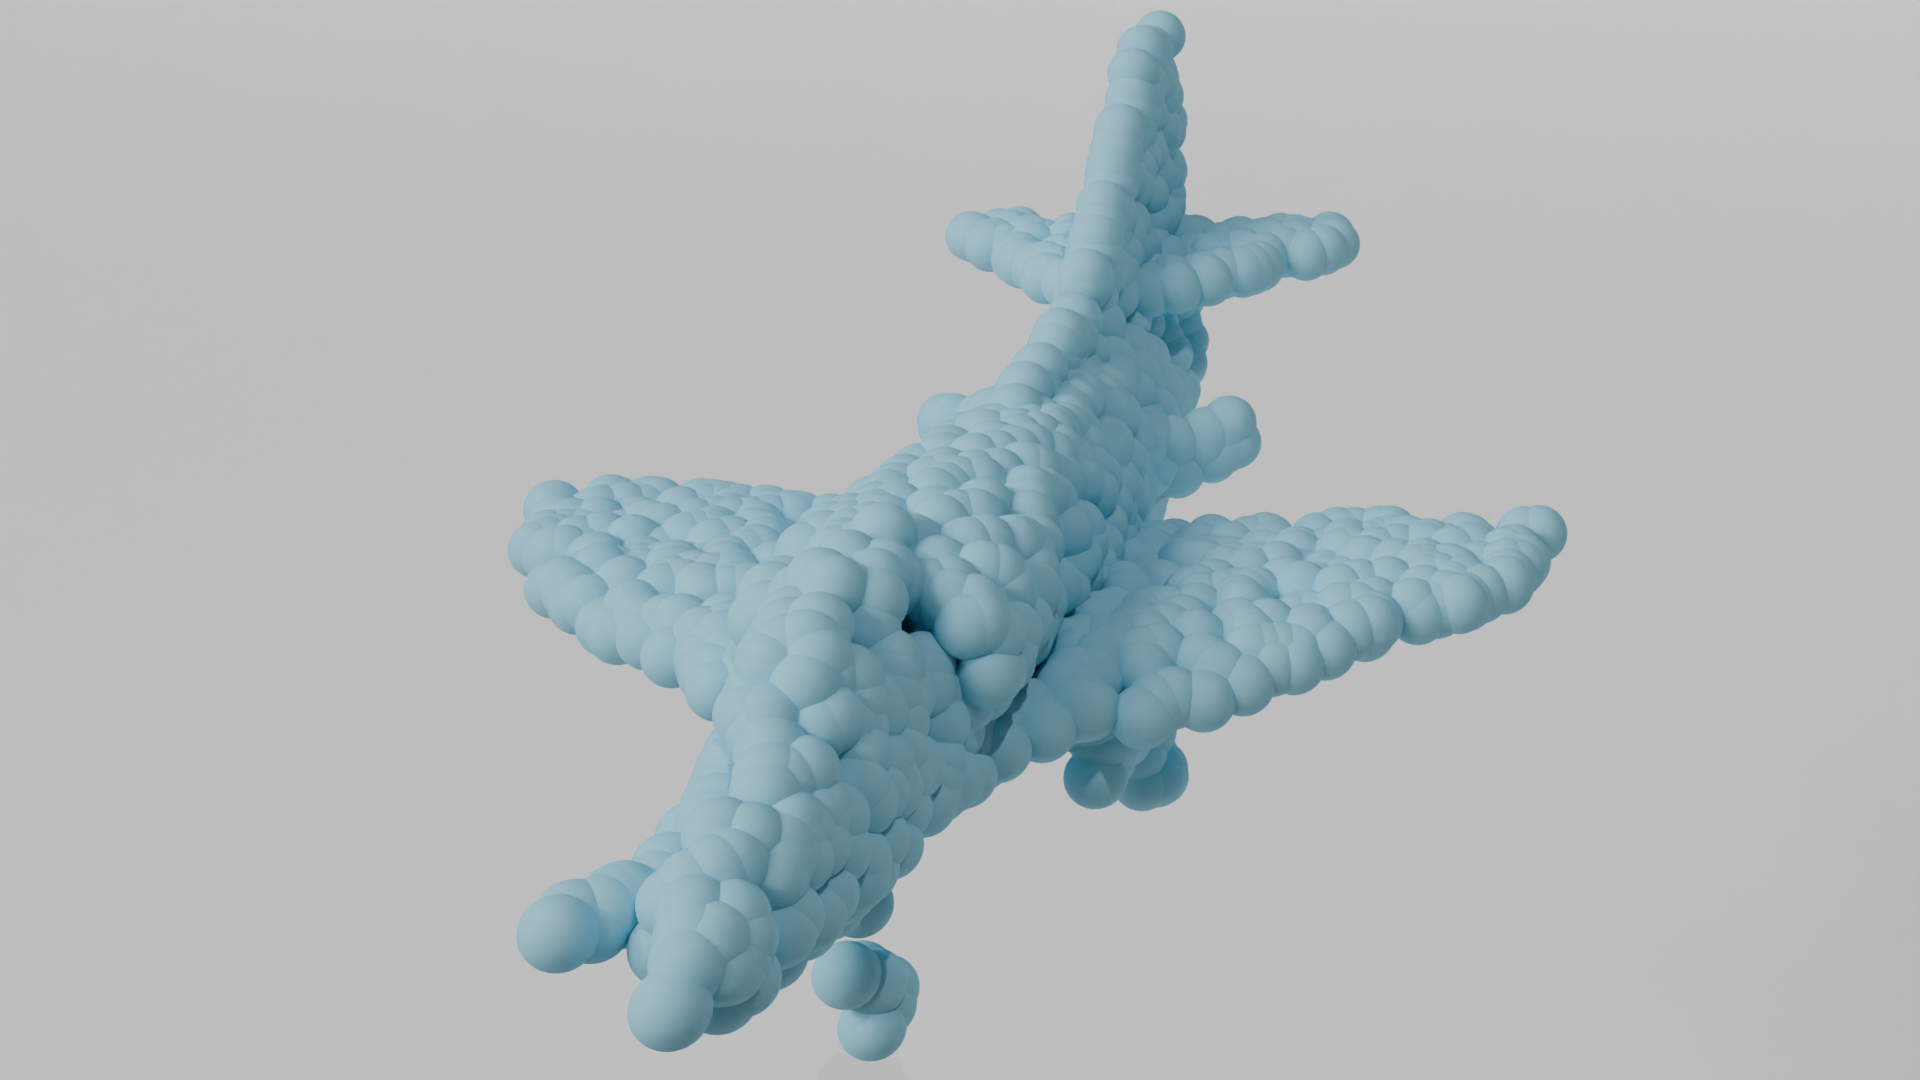
\includegraphics[width=\textwidth]{figures/com_ap3.png}
            \caption{Airplane 3}
          \end{subfigure}
          \caption{Qualitative comparison between different empirical uncertainty quantification methods for point cloud completion on the airplane subcategory of ShapeNet data. Input refers to the partial point cloud, and GT refers to the ground truth complete cloud. DropCon, Dropout, Ensemble, and Implicit refer to the uncertainty maps output by the DropConnect, dropout, deep ensemble, and implicit generative model-based methods, respectively.}
          \label{fig:airplane}
        \end{figure}
        \newline
        
        As seen in Figure~\ref{fig:airplane}, the DropConnect-based model was not able to learn to generate shapes consistent with the ground truth. Such behaviour can be attributed to either suboptimal training or the fact that each weight in the network is important in predicting the encoding for generated shapes, and dropping them in inference time affects the quality. The other models generated consistent, completed shapes but differed in terms of diversity and fidelity to the partial cloud. The ensemble of generators and dropout-based models produced completed shapes that were only diverse in the geometrically complex regions and overall consistent with the partial point clouds. The dropout-based models generated a bit more diverse shapes compared to an ensemble of generators. The generative implicit models produced the most diverse completions with more uncertainty in both geometrically complex and incomplete (with respect to partial cloud) regions. It also captured that certain regions are expected not to vary significantly, regardless of the sparsity in the input cloud. However, due to the variety of completions, the average completed shape deviated slightly from the partial cloud. A similar pattern can be seen in the results of the table subcategory shown in Figure~\ref{fig:table}.
        
        \begin{figure}[htb]
          \centering
          \begin{subfigure}[t]{\dimexpr0.315\textwidth+20pt\relax}
            \makebox[20pt]{\raisebox{30pt}{\rotatebox[origin=c]{90}{\small Input}}}%
            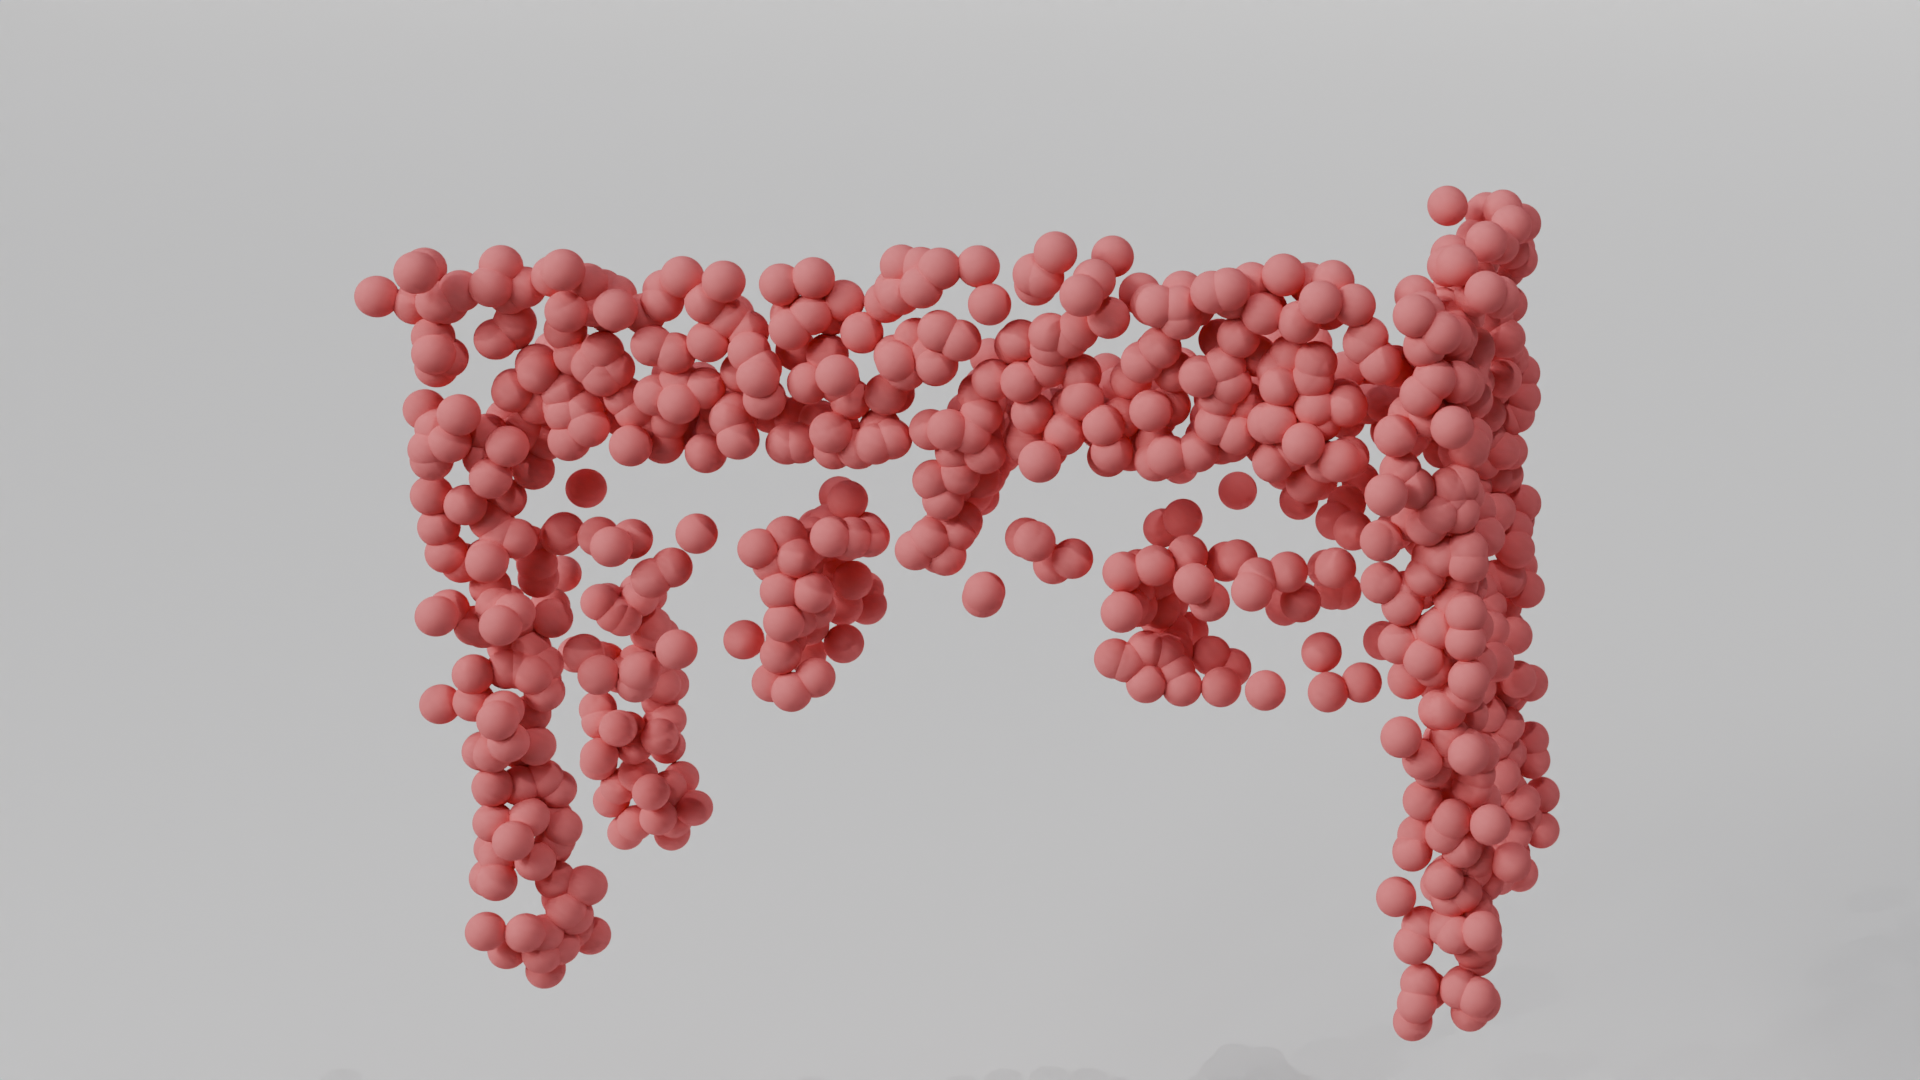
\includegraphics[width=\dimexpr\linewidth-20pt\relax]{figures/part_t1.png}
            \makebox[20pt]{\raisebox{30pt}{\rotatebox[origin=c]{90}{\small DropCon}}}%
            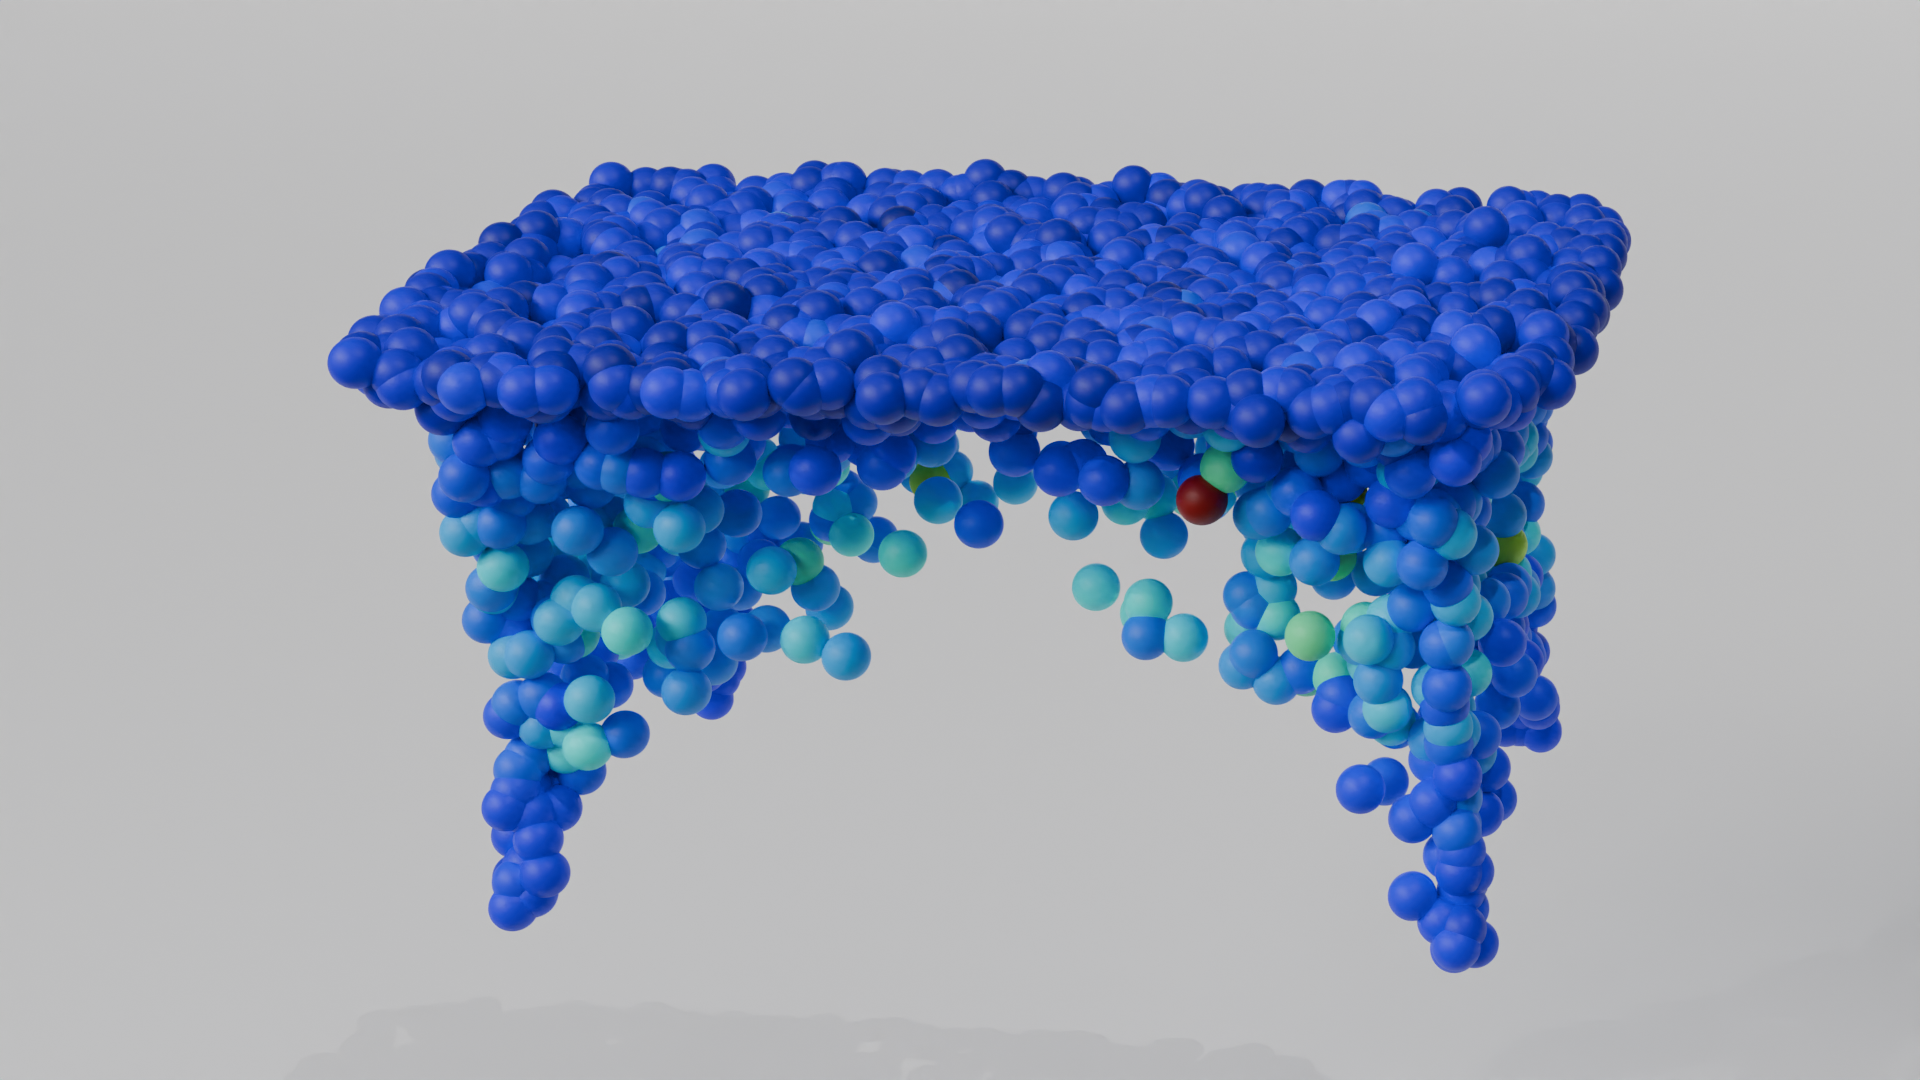
\includegraphics[width=\dimexpr\linewidth-20pt\relax]{figures/dc_lin_t1.png}
            \makebox[20pt]{\raisebox{30pt}{\rotatebox[origin=c]{90}{\small Dropout}}}%
            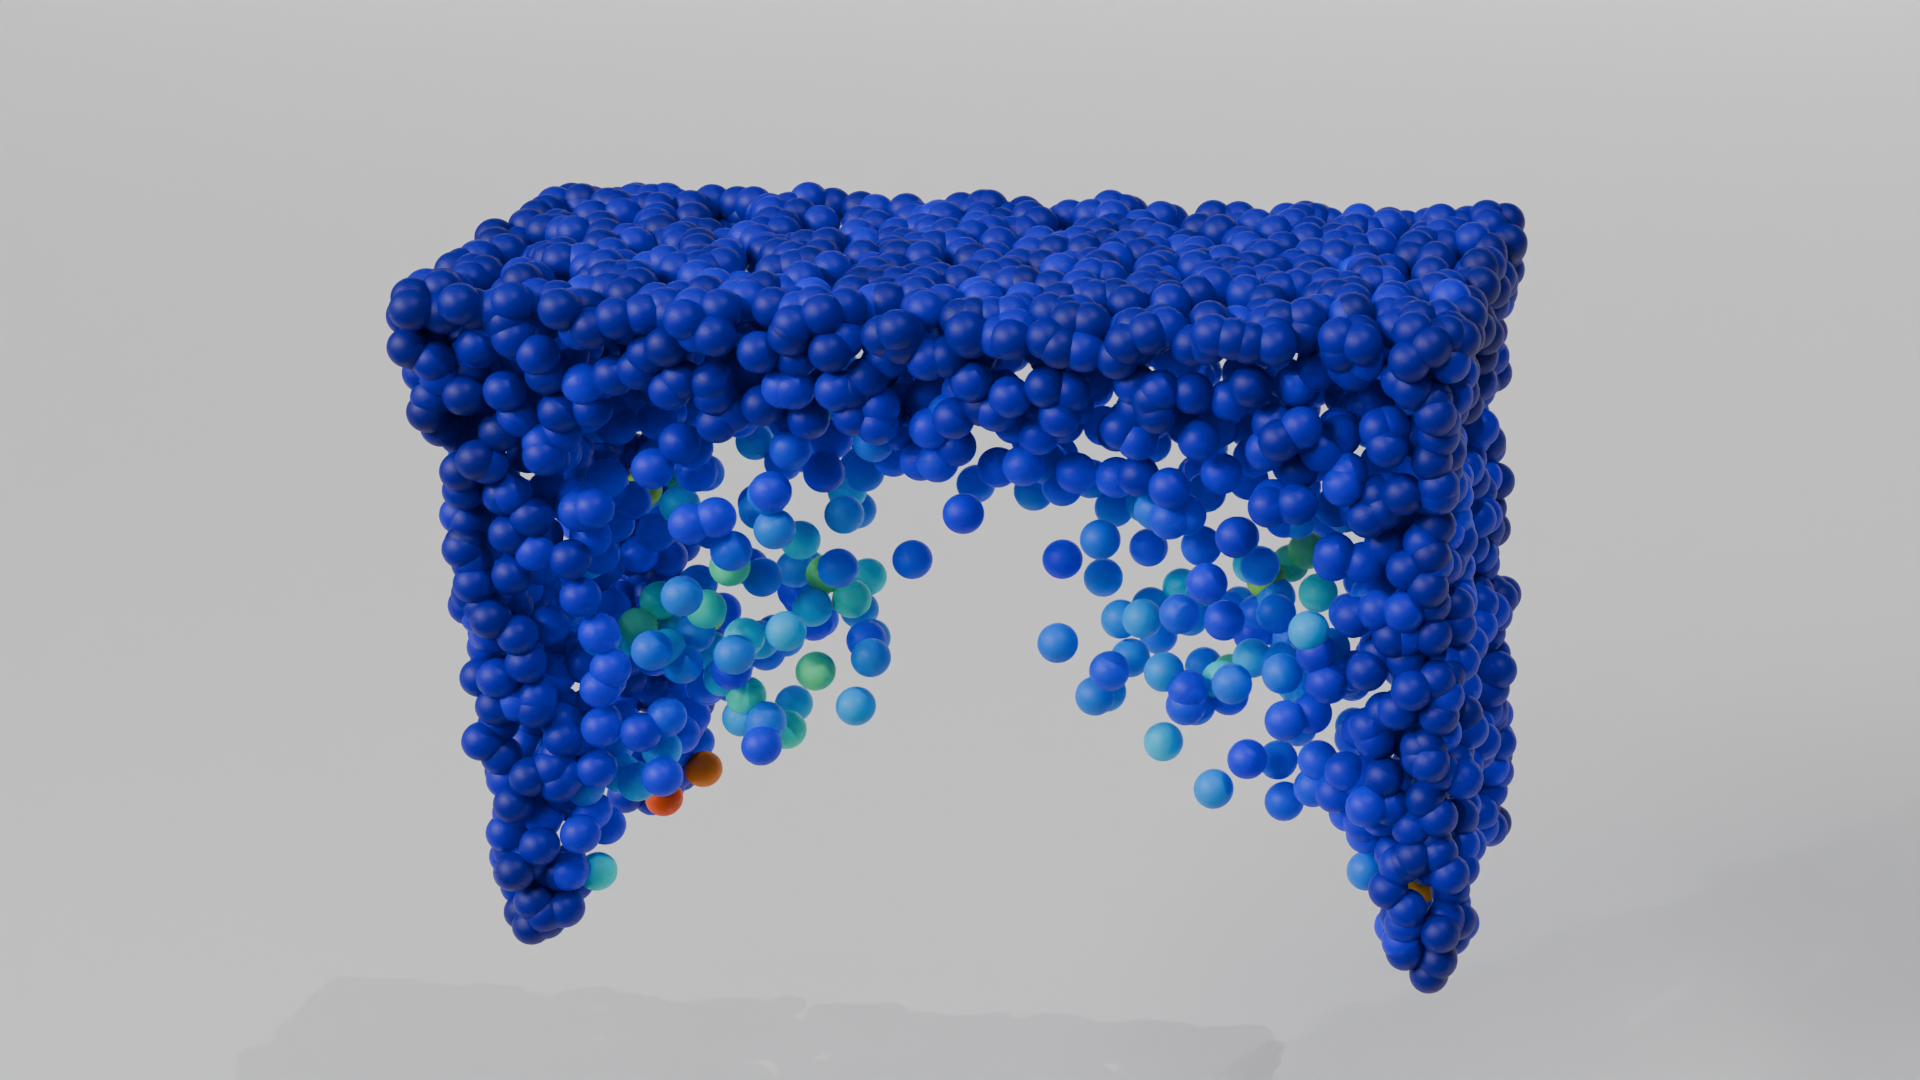
\includegraphics[width=\dimexpr\linewidth-20pt\relax]{figures/do_lin_t1.png}
            \makebox[20pt]{\raisebox{30pt}{\rotatebox[origin=c]{90}{\small Ensemble}}}%
            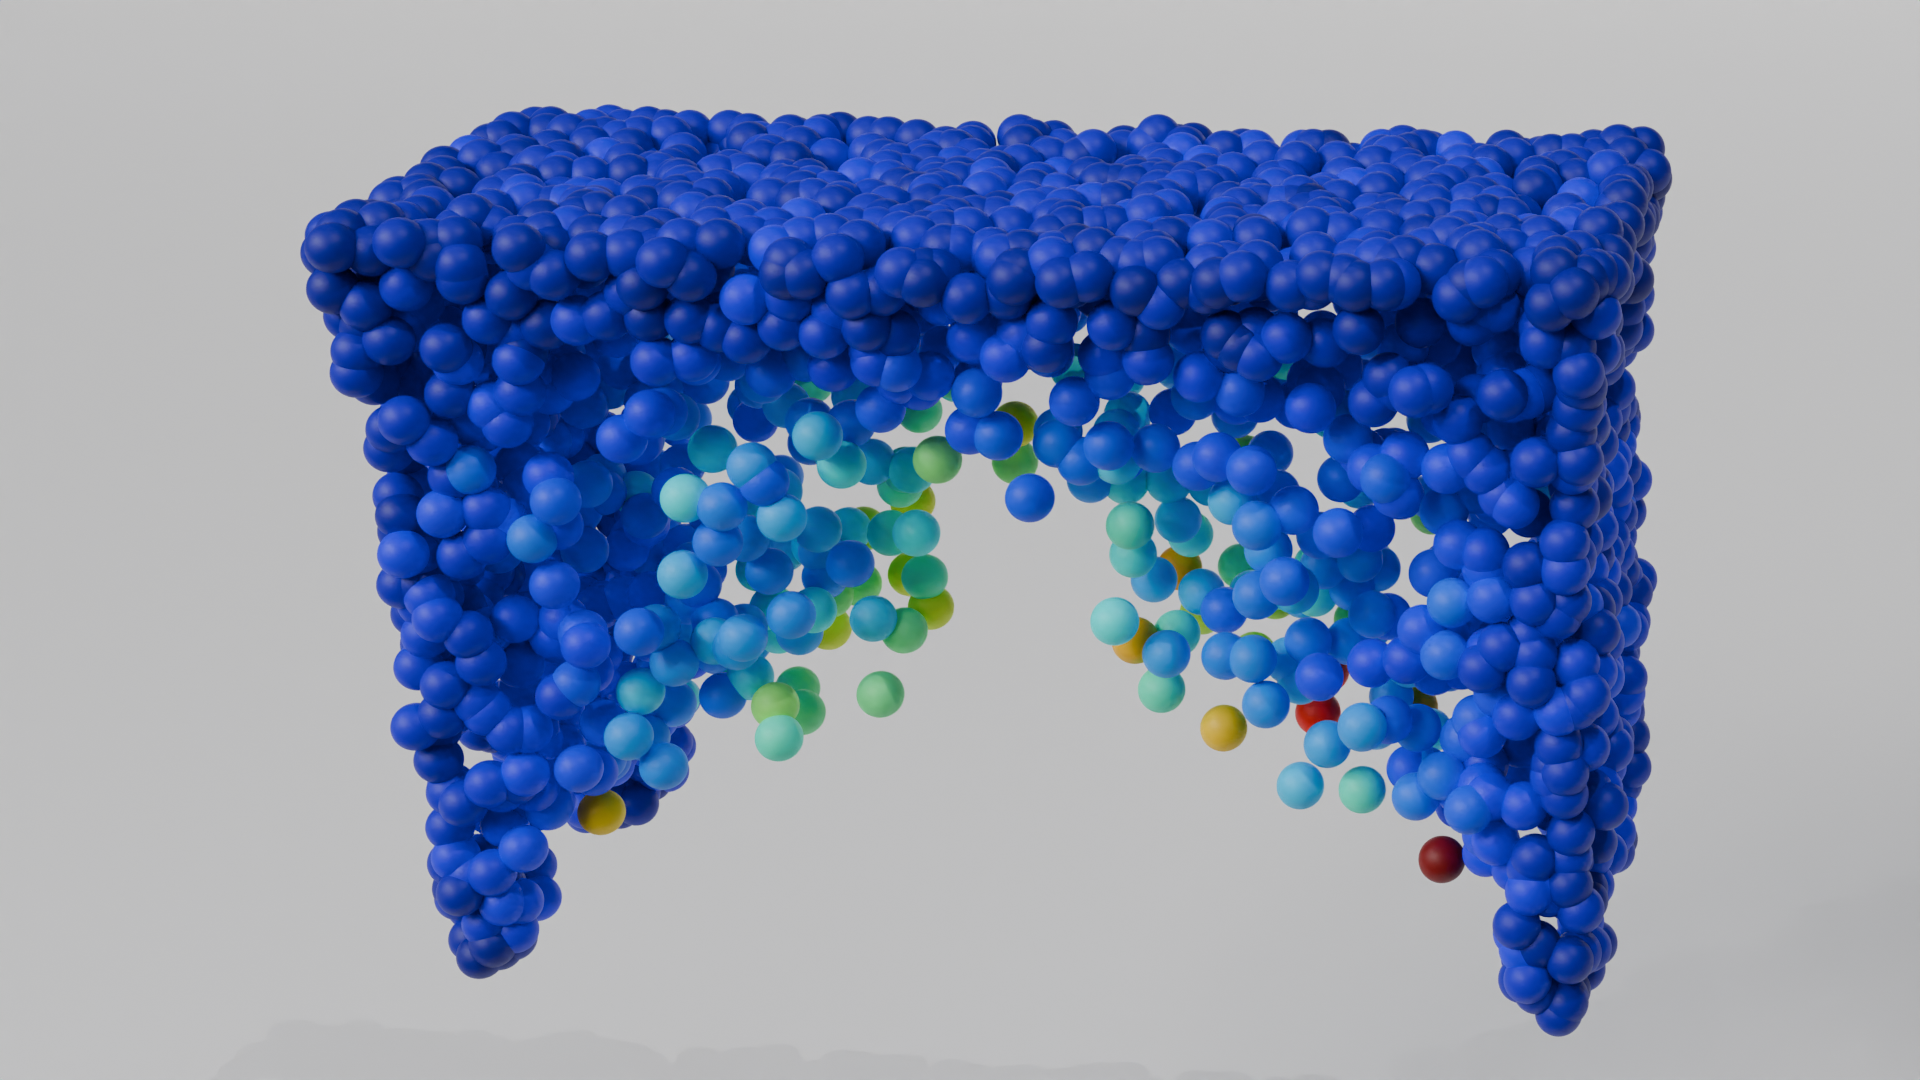
\includegraphics[width=\dimexpr\linewidth-20pt\relax]{figures/ens_lin_t1.png}
            \makebox[20pt]{\raisebox{30pt}{\rotatebox[origin=c]{90}{\small Implicit}}}%
            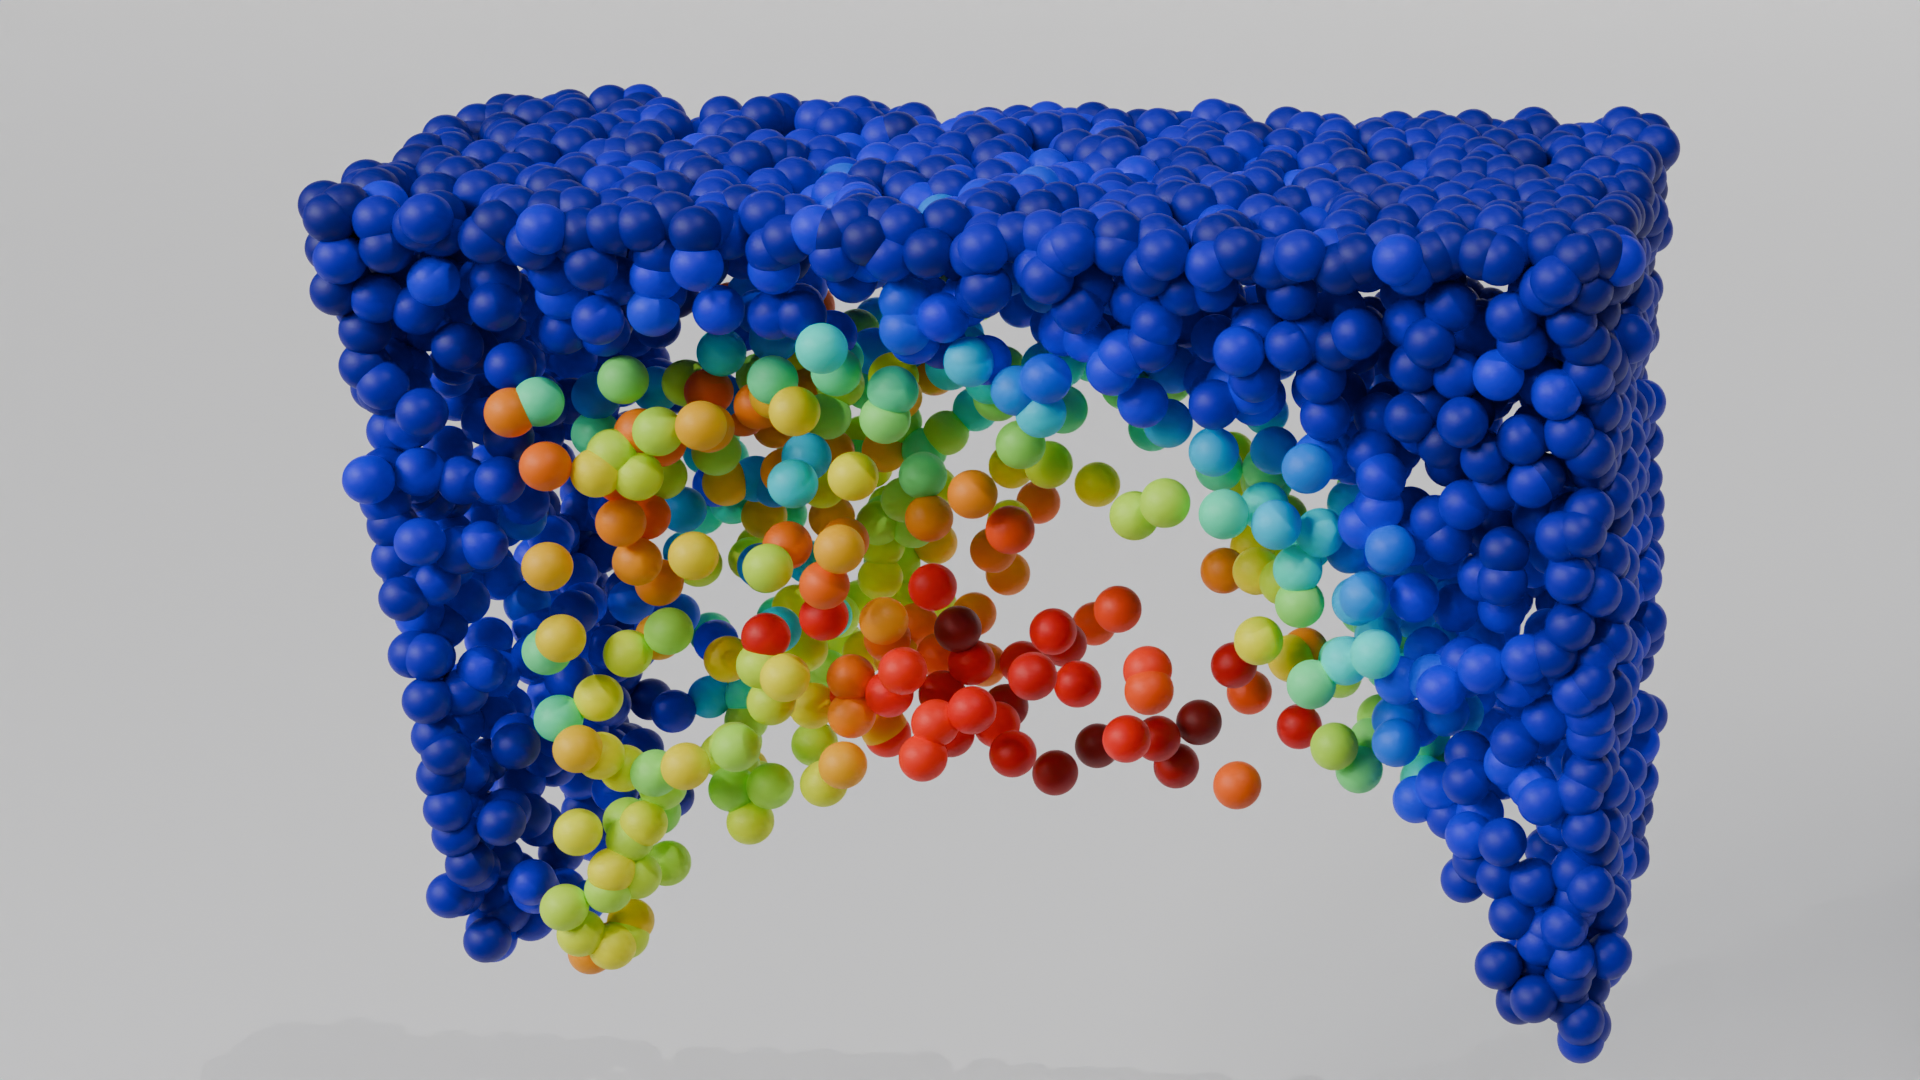
\includegraphics[width=\dimexpr\linewidth-20pt\relax]{figures/iml_lin_t1.png}
            \makebox[20pt]{\raisebox{30pt}{\rotatebox[origin=c]{90}{\small GT}}}%
            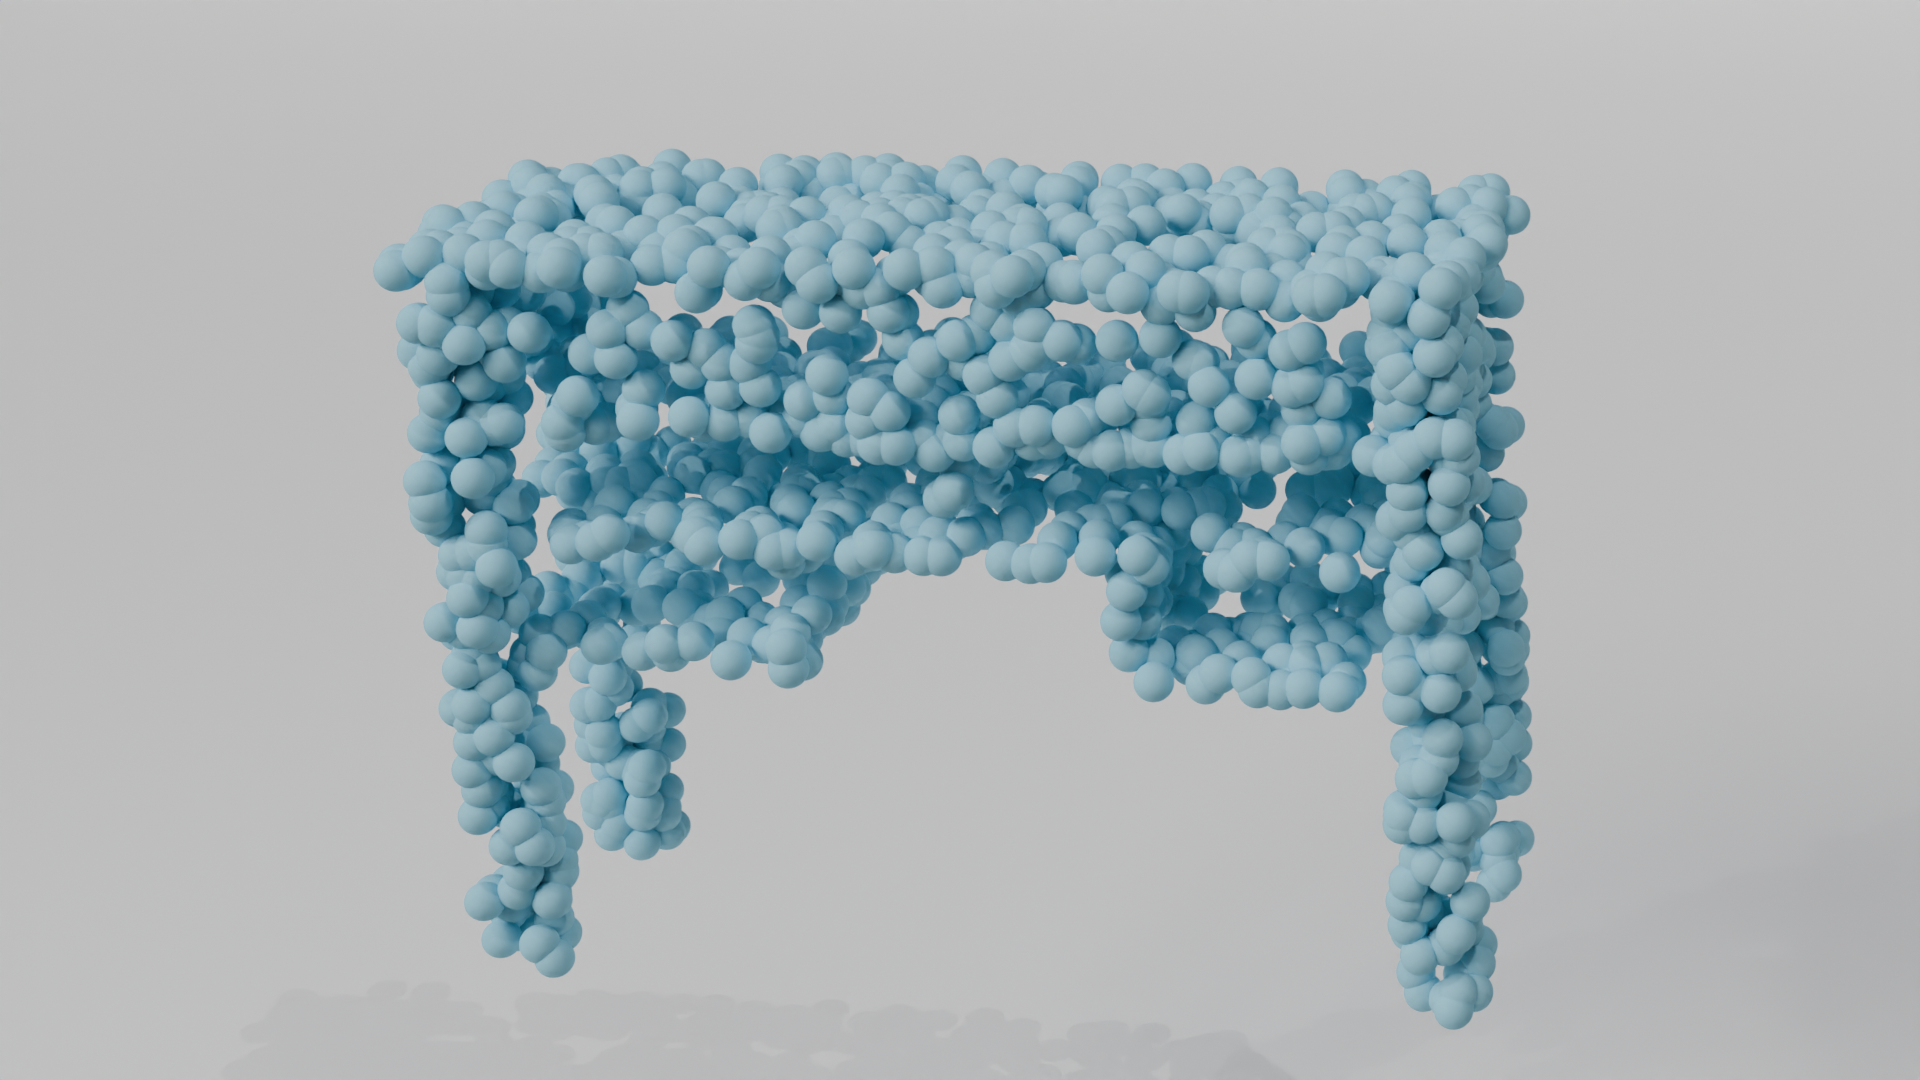
\includegraphics[width=\dimexpr\linewidth-20pt\relax]{figures/com_t1.png}
            \caption{Table 1}
          \end{subfigure}\hfill
          \begin{subfigure}[t]{0.315\textwidth}
            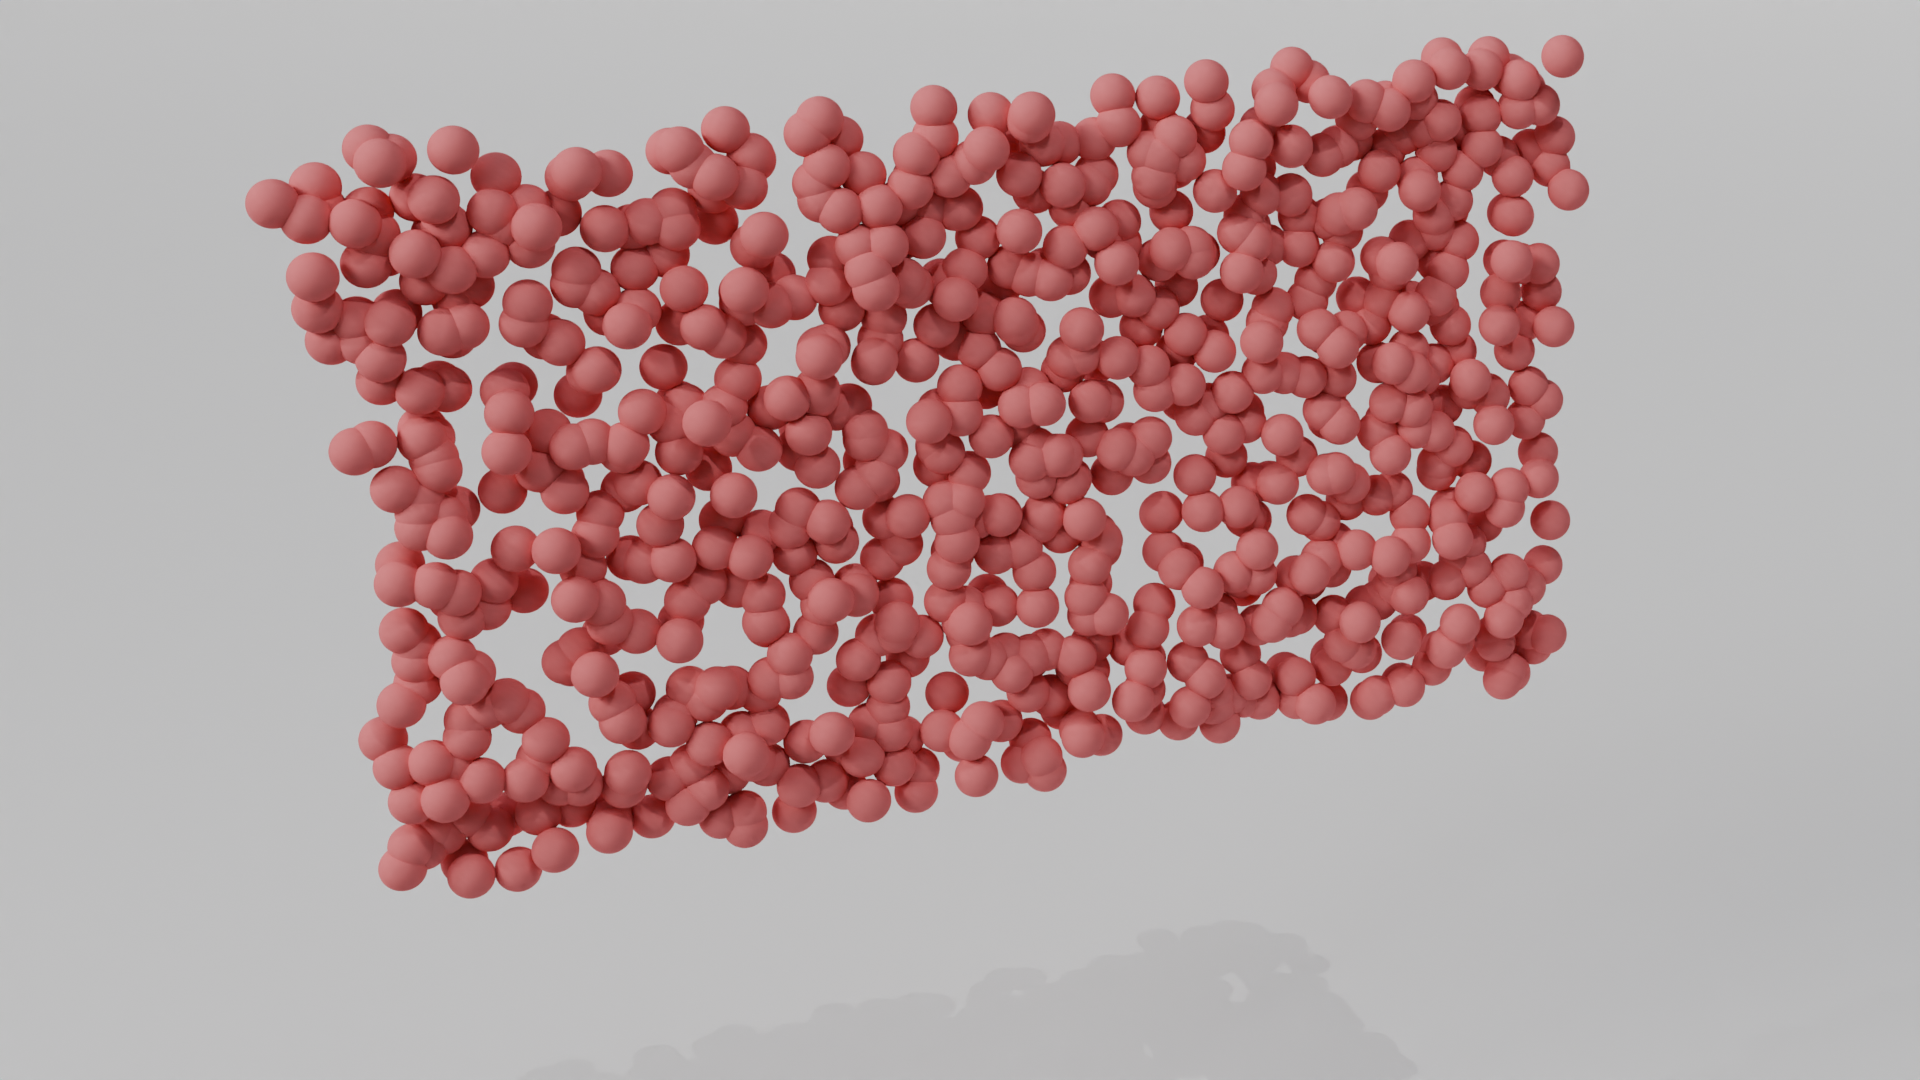
\includegraphics[width=\textwidth]{figures/part_t2.png}
            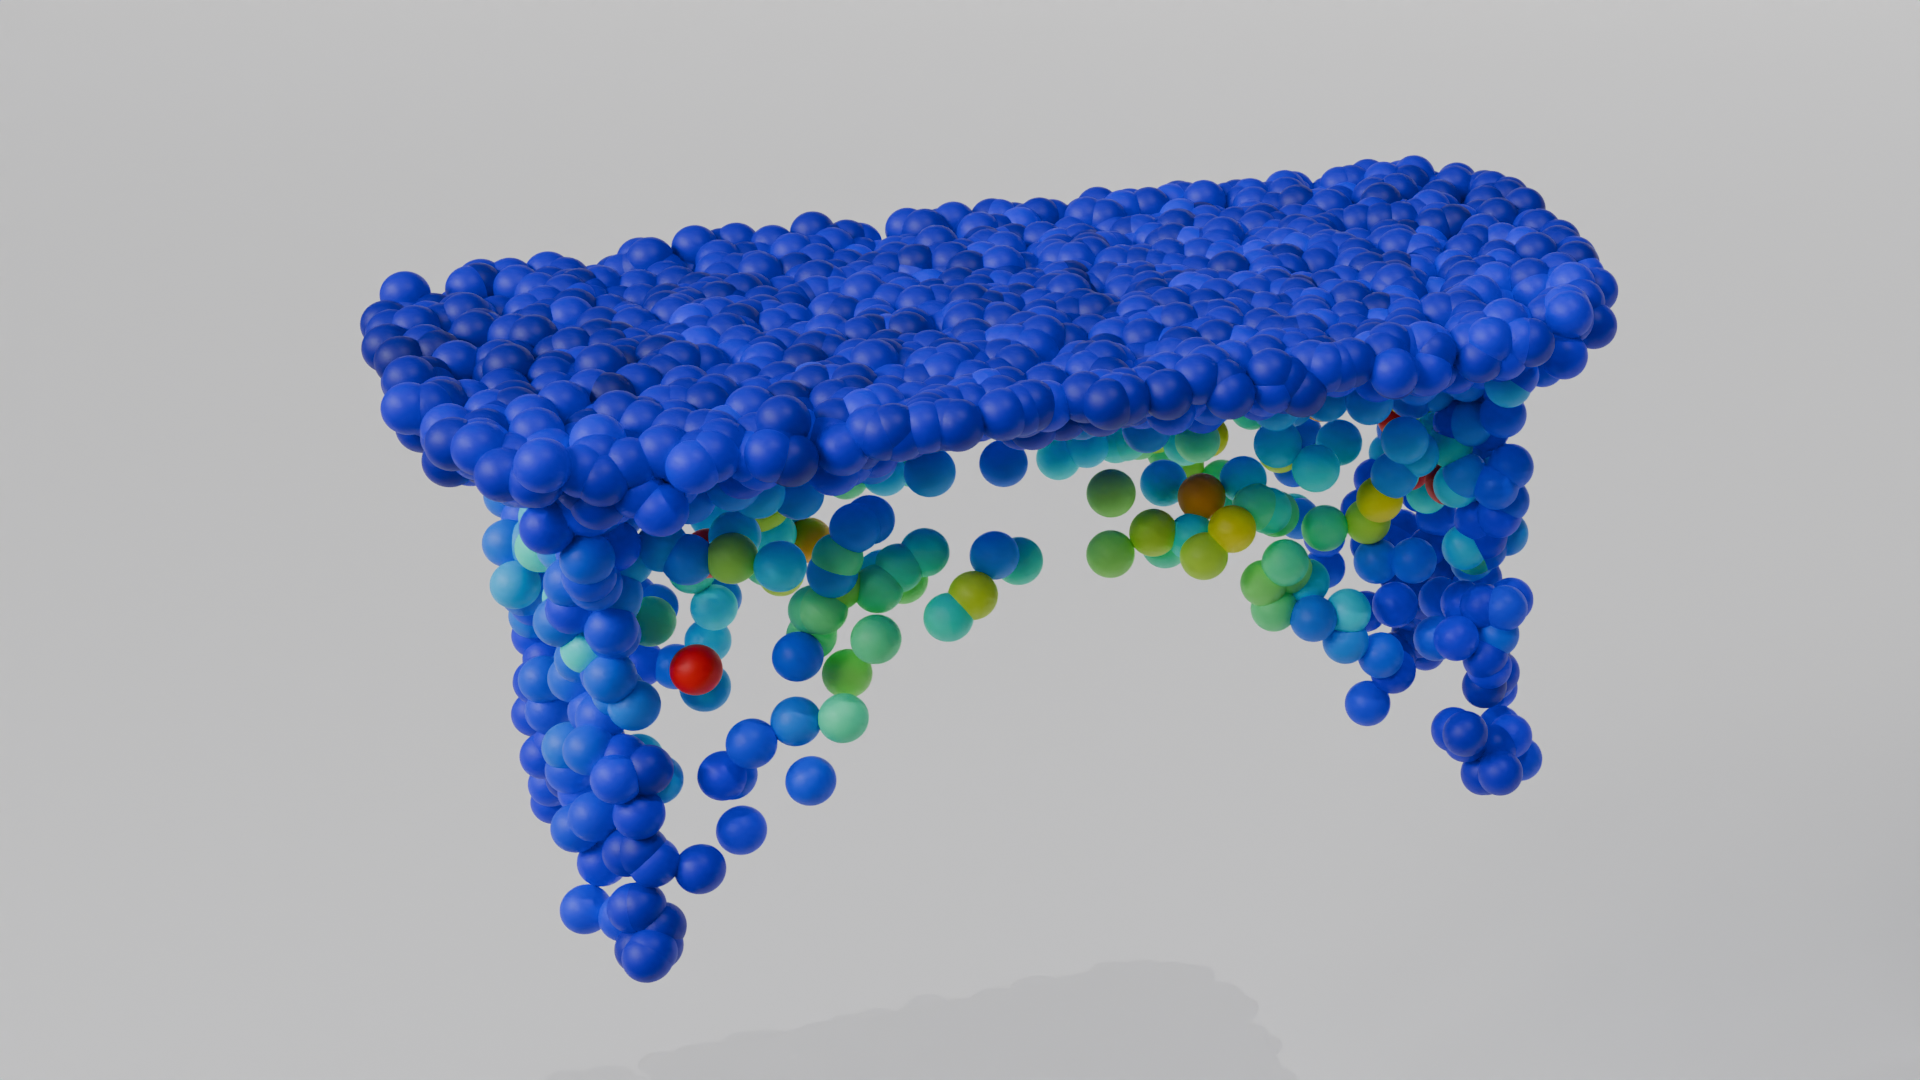
\includegraphics[width=\textwidth]{figures/dc_lin_t2.png}
            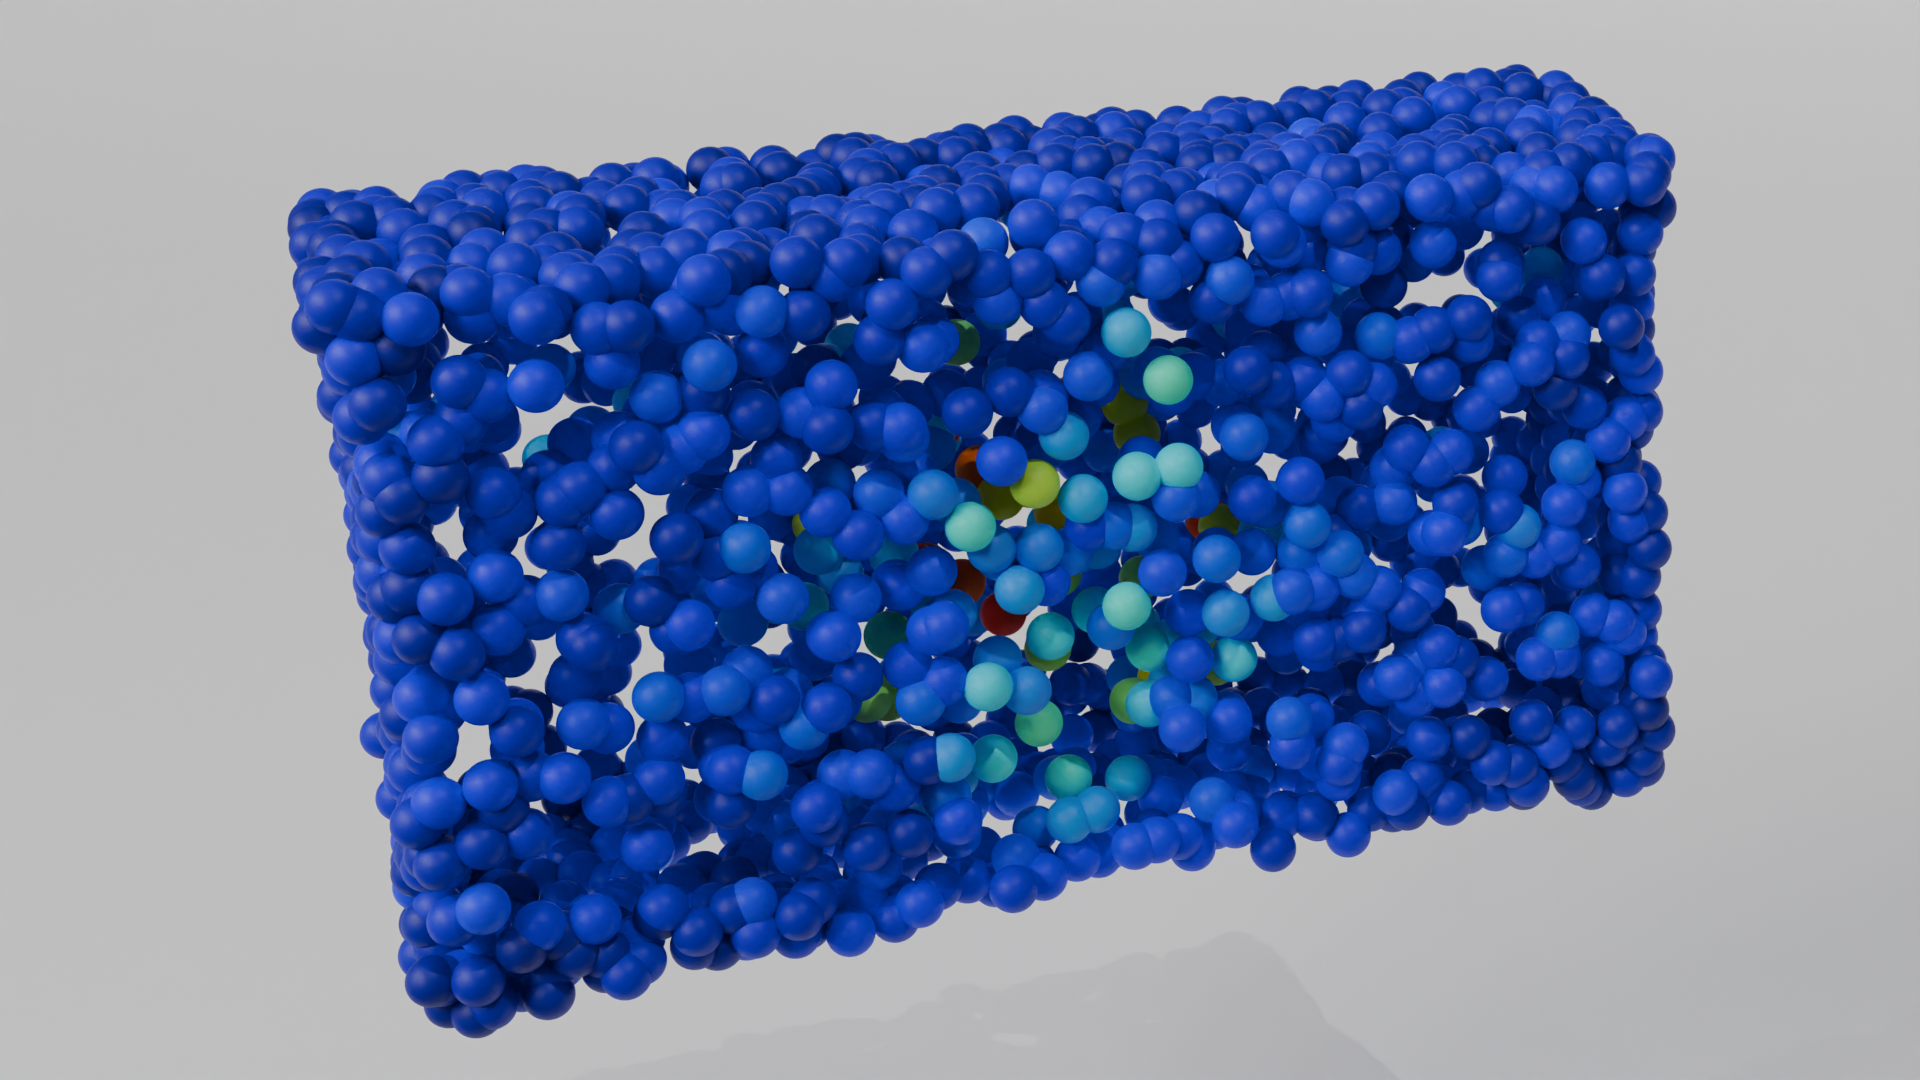
\includegraphics[width=\textwidth]{figures/do_lin_t2.png}
            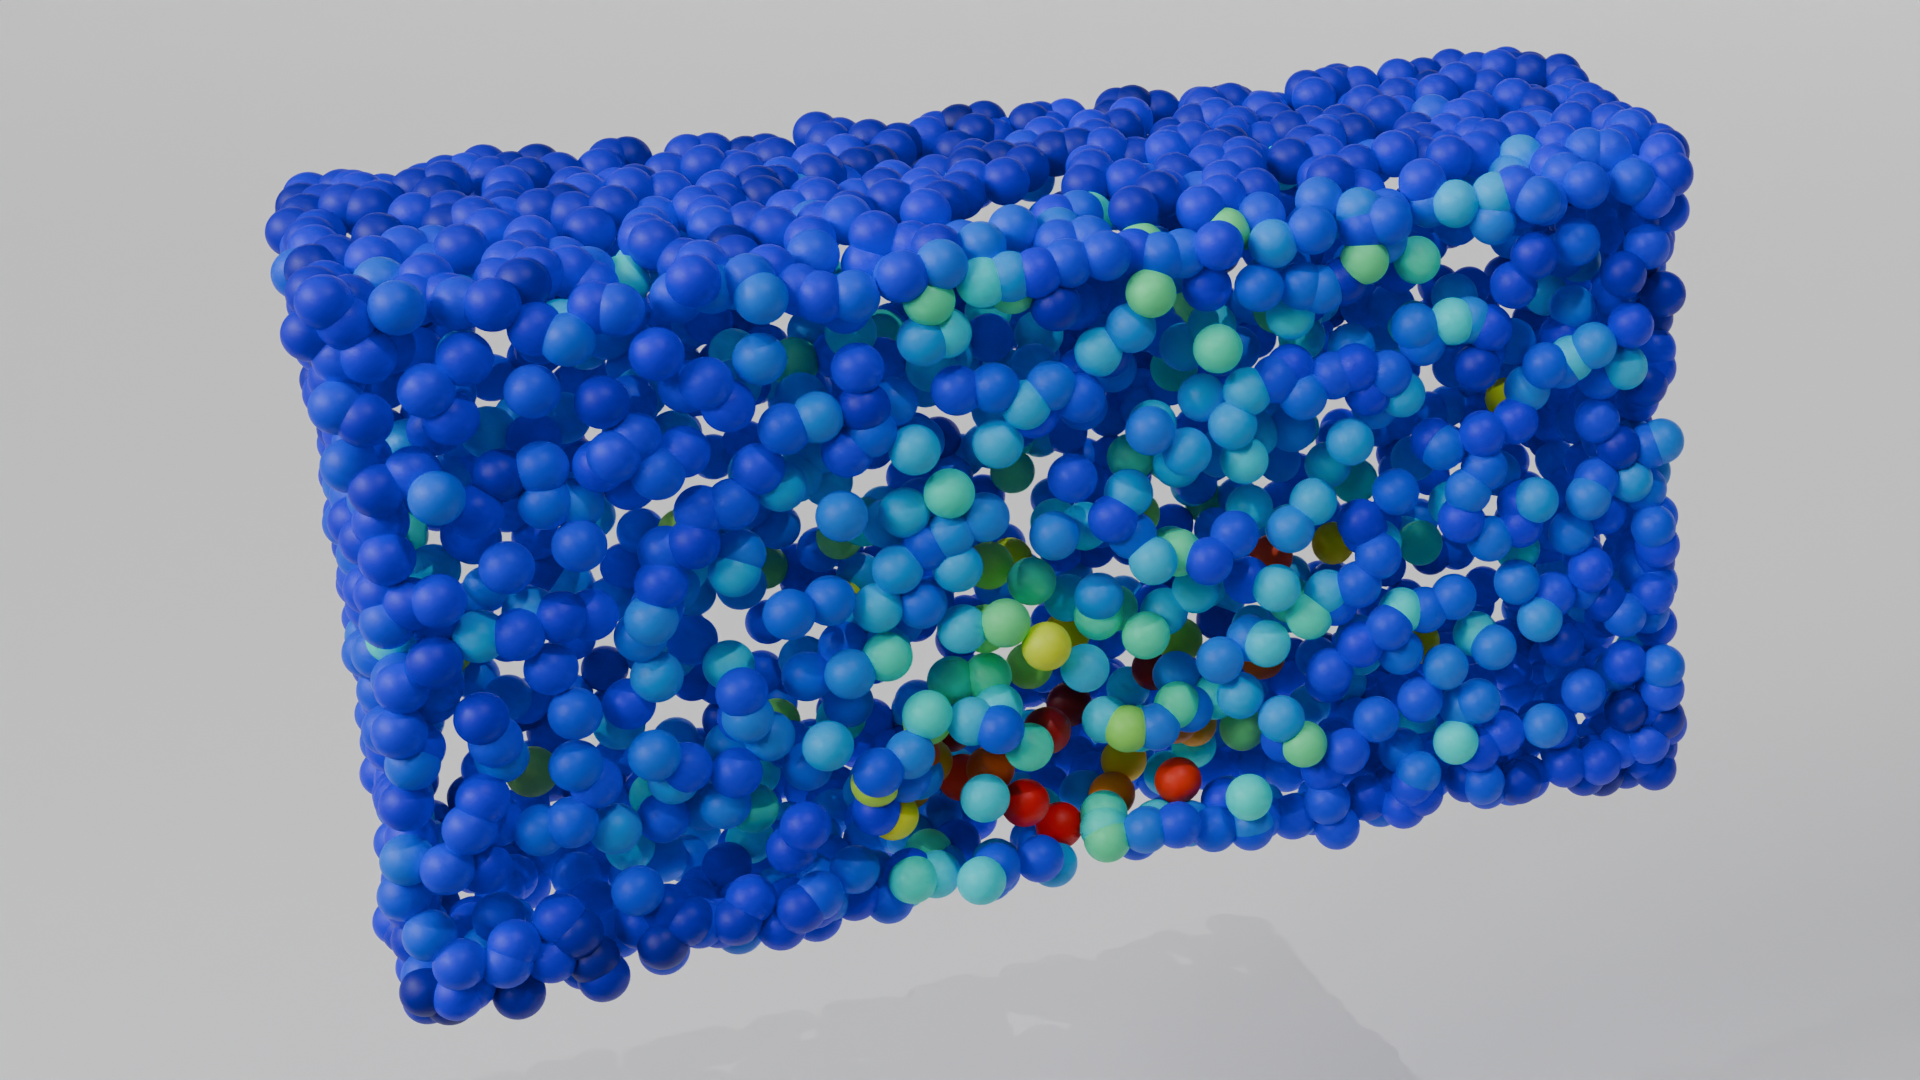
\includegraphics[width=\textwidth]{figures/ens_lin_t2.png}
            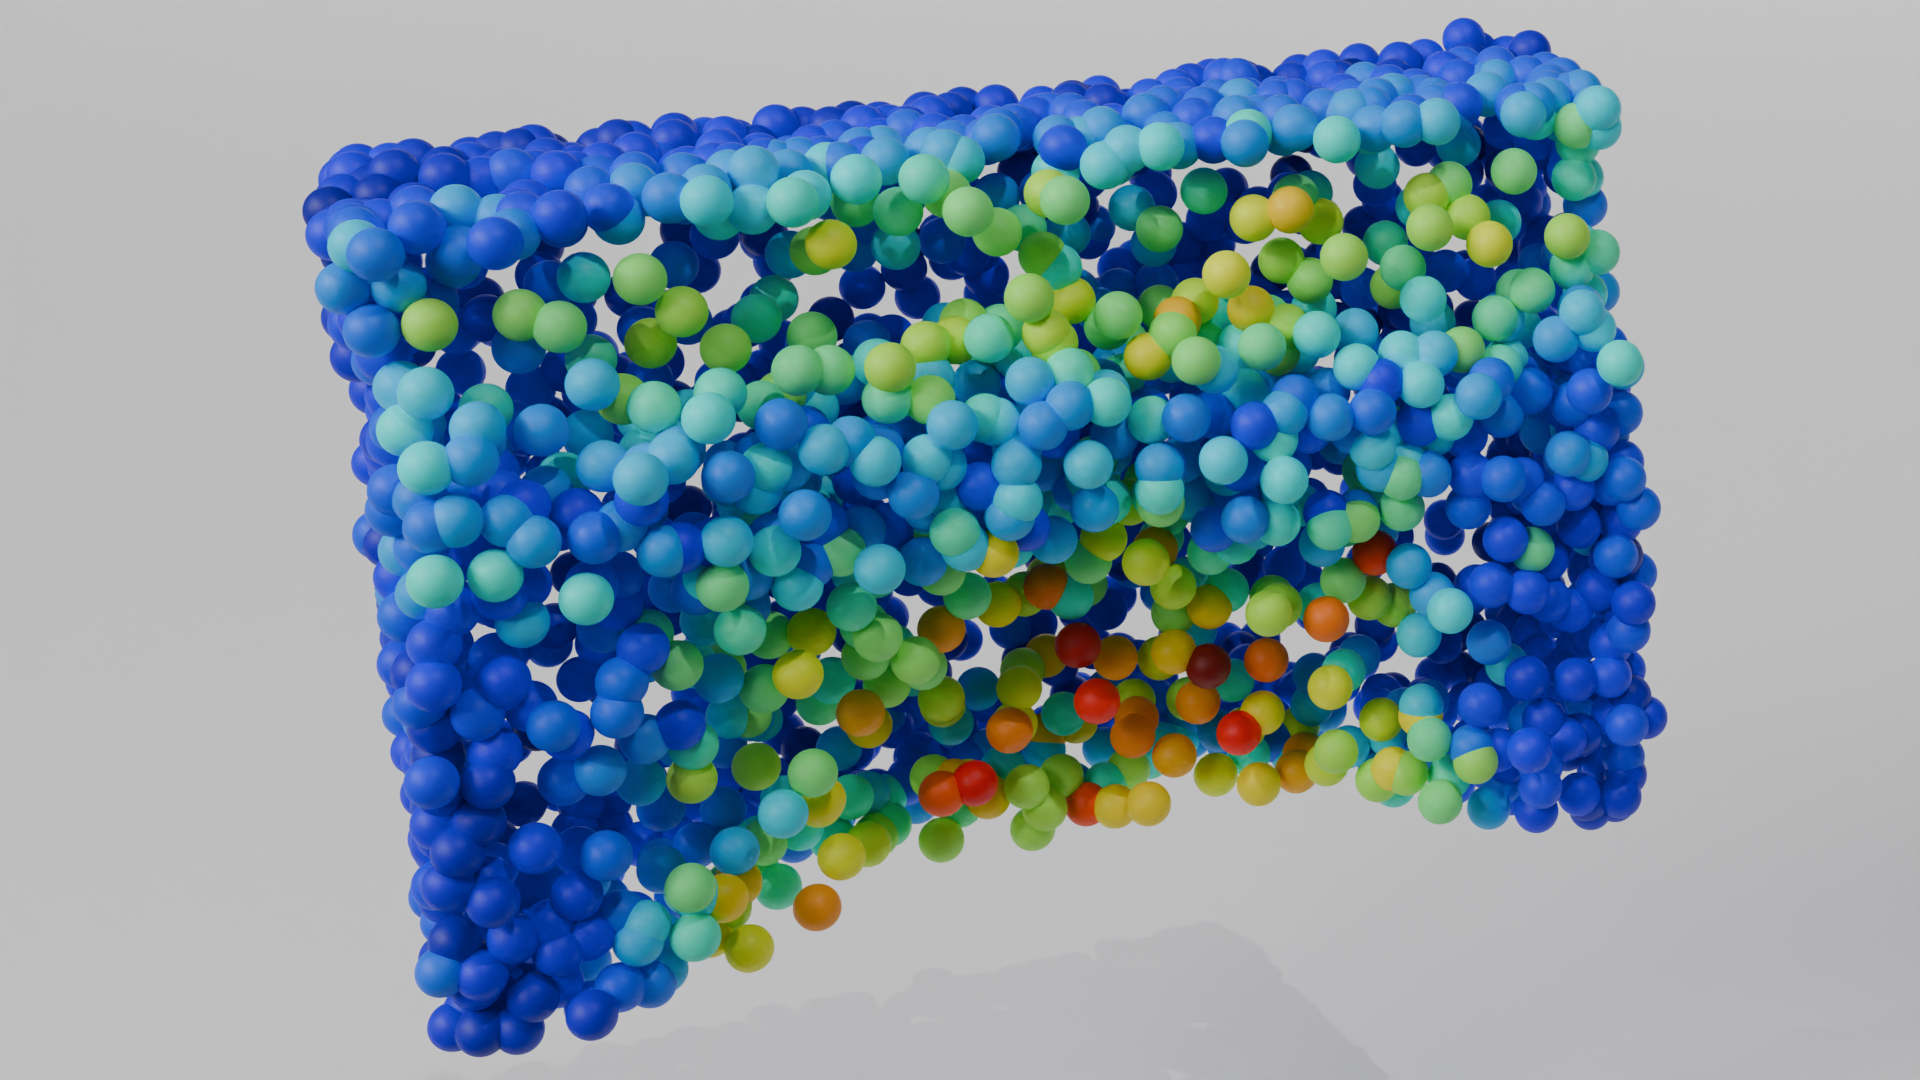
\includegraphics[width=\textwidth]{figures/iml_lin_t2.png}
            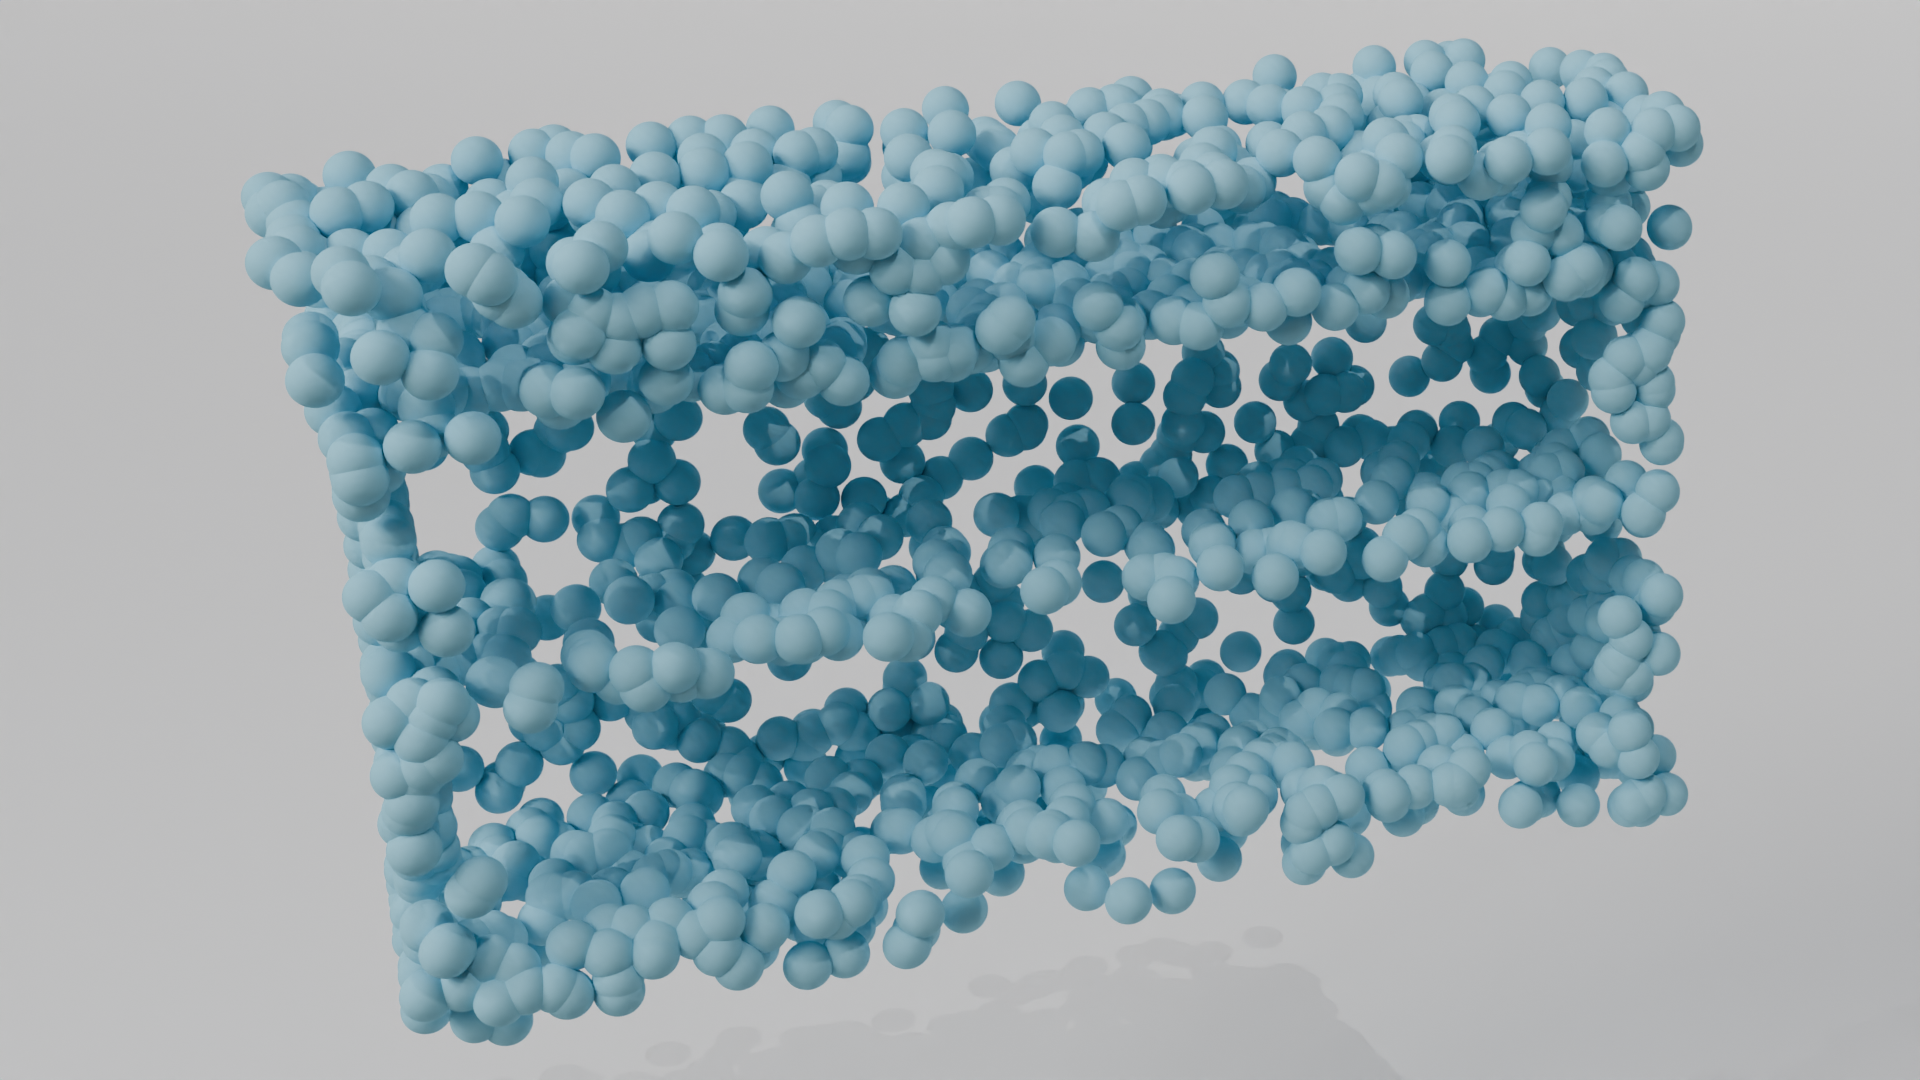
\includegraphics[width=\textwidth]{figures/com_t2.png}
            \caption{Table 2}
          \end{subfigure}\hfill
          \begin{subfigure}[t]{0.315\textwidth}
            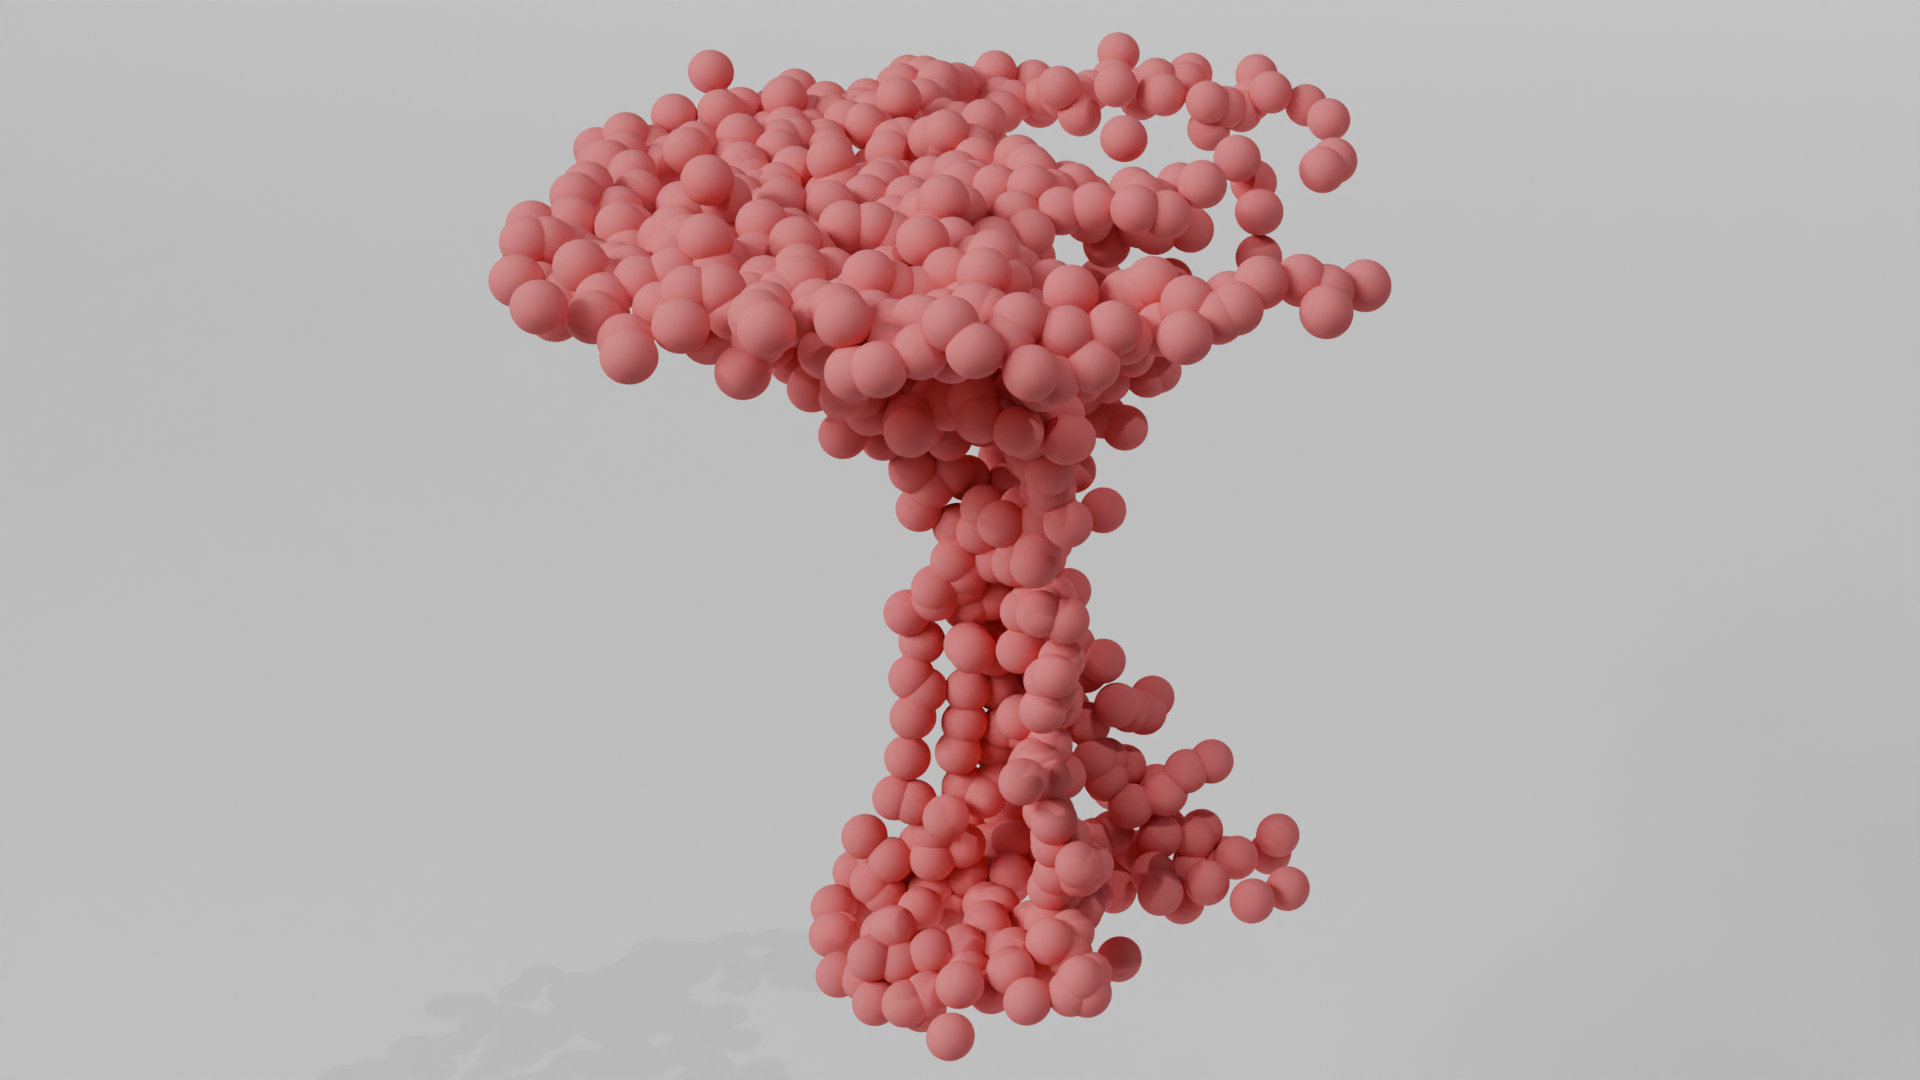
\includegraphics[width=\textwidth]{figures/part_t3.png}
            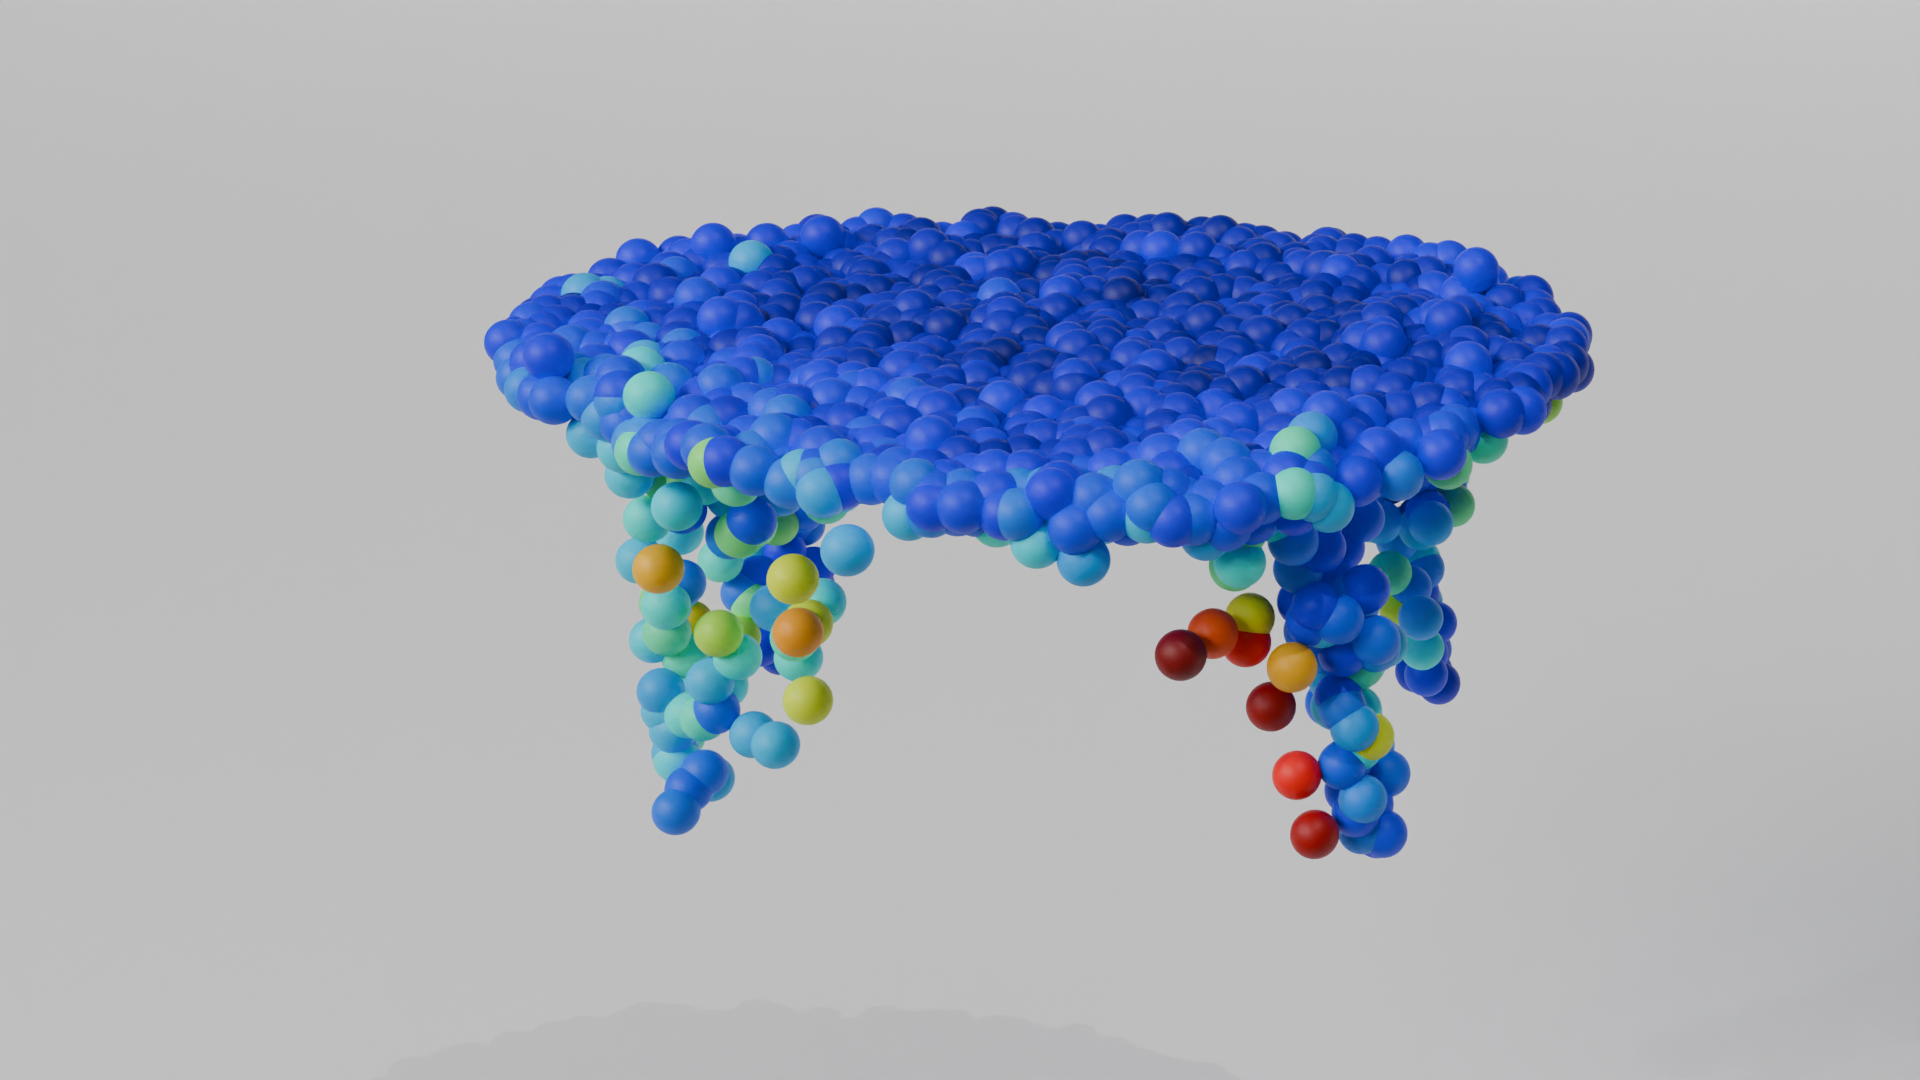
\includegraphics[width=\textwidth]{figures/dc_lin_t3.png}
            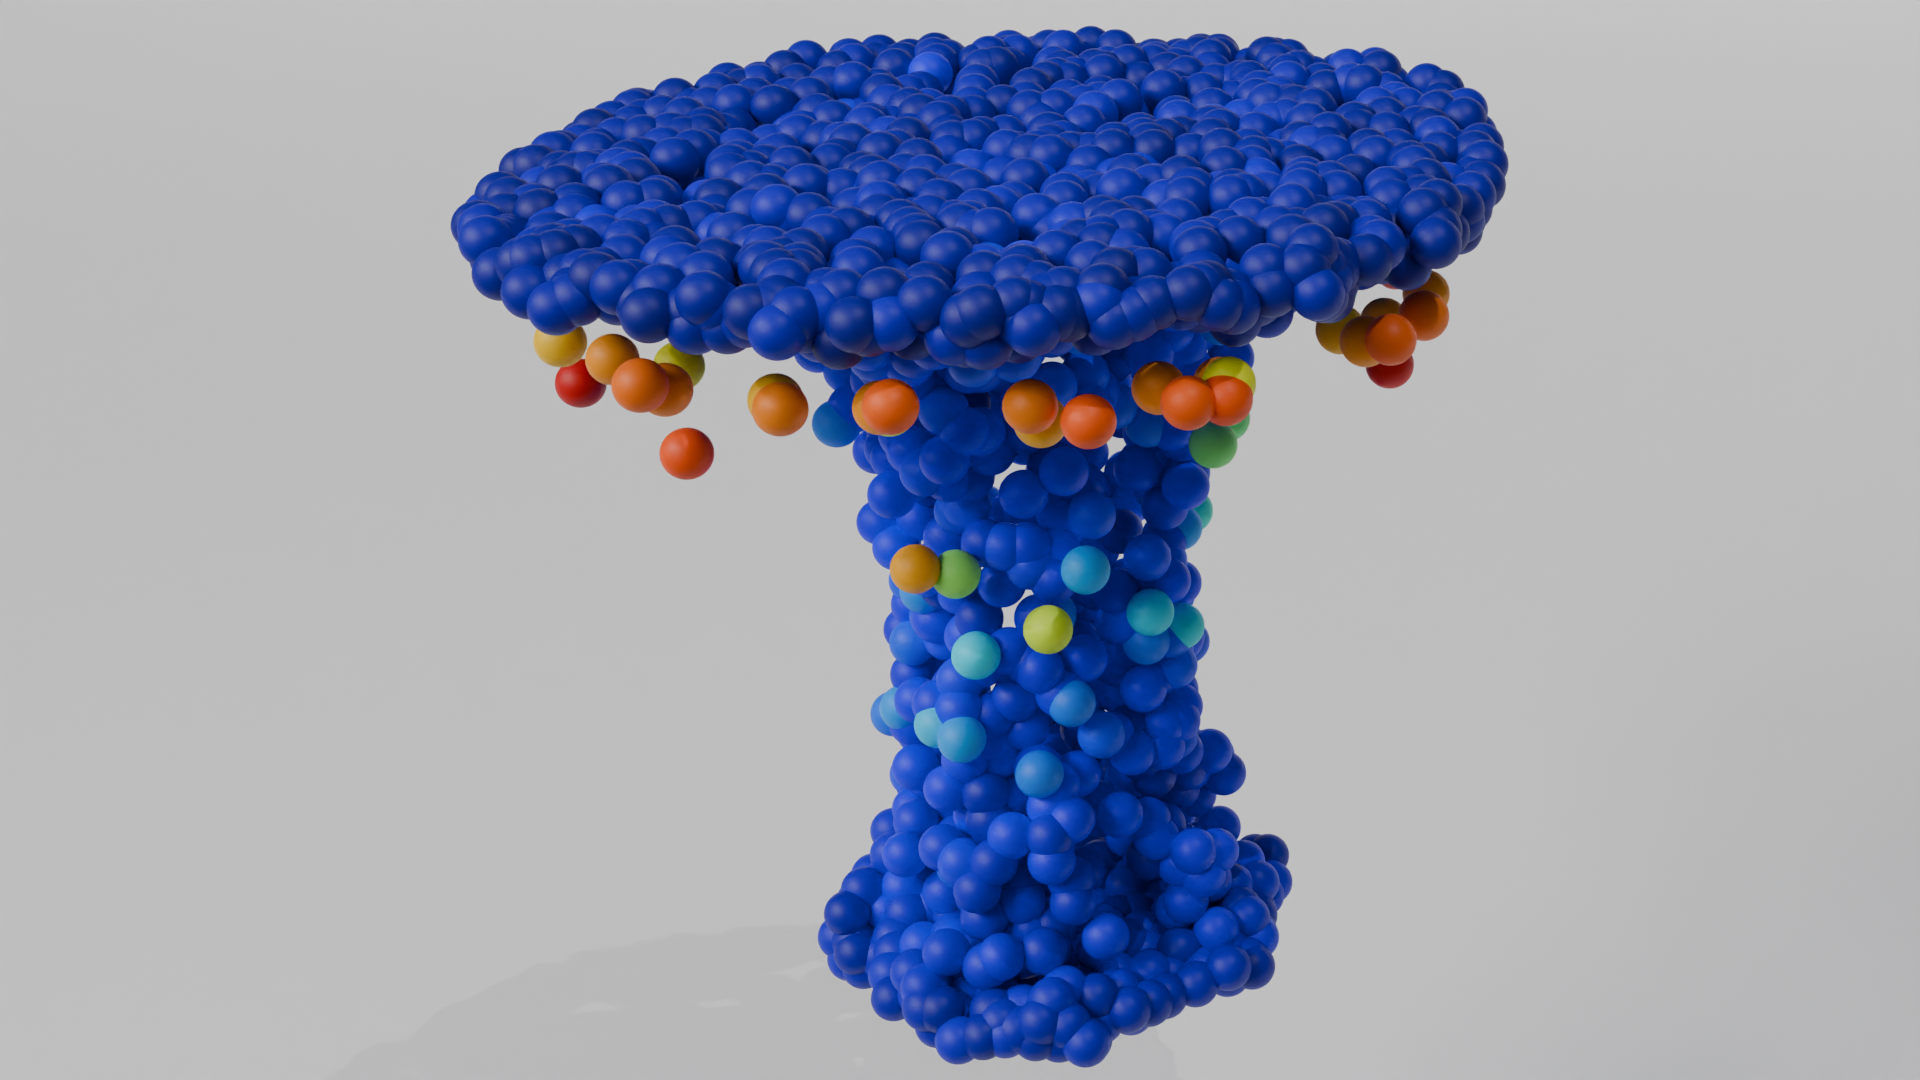
\includegraphics[width=\textwidth]{figures/do_lin_t3.png}
            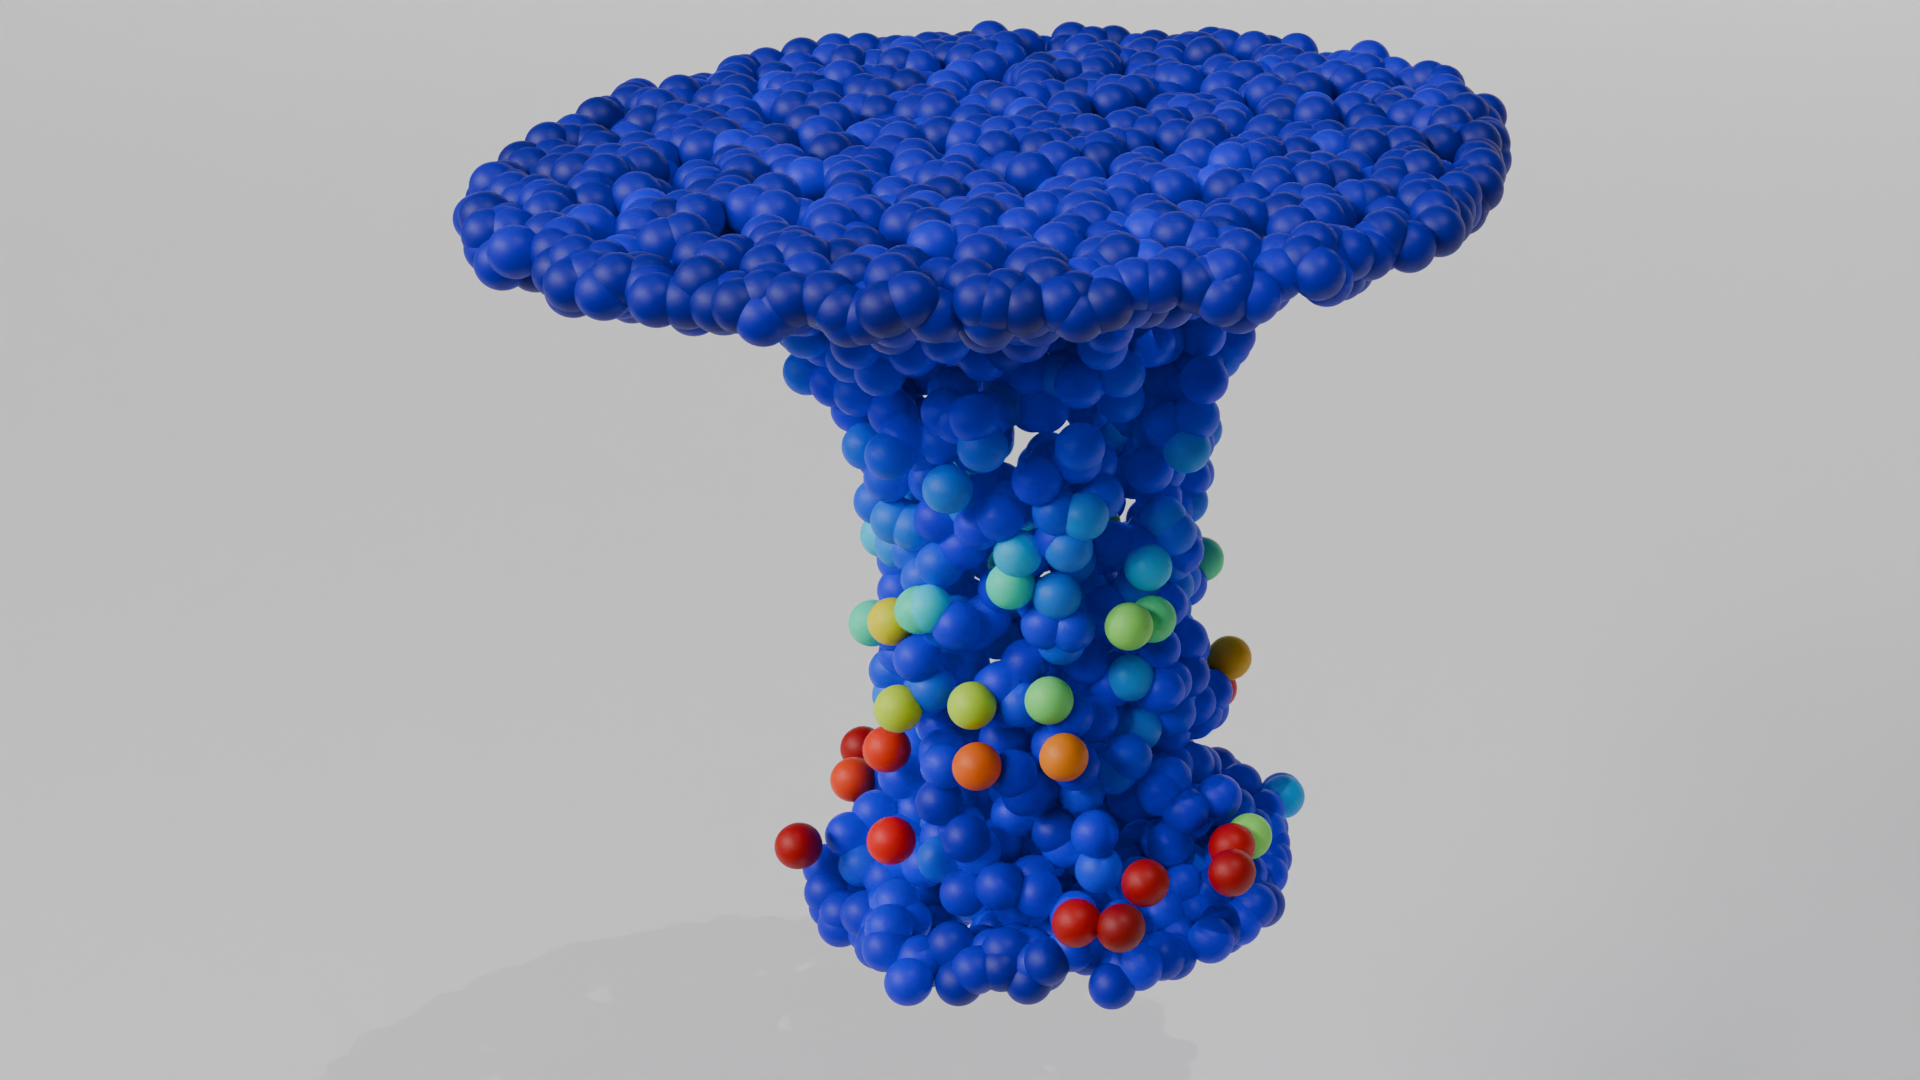
\includegraphics[width=\textwidth]{figures/ens_lin_t3.png}
            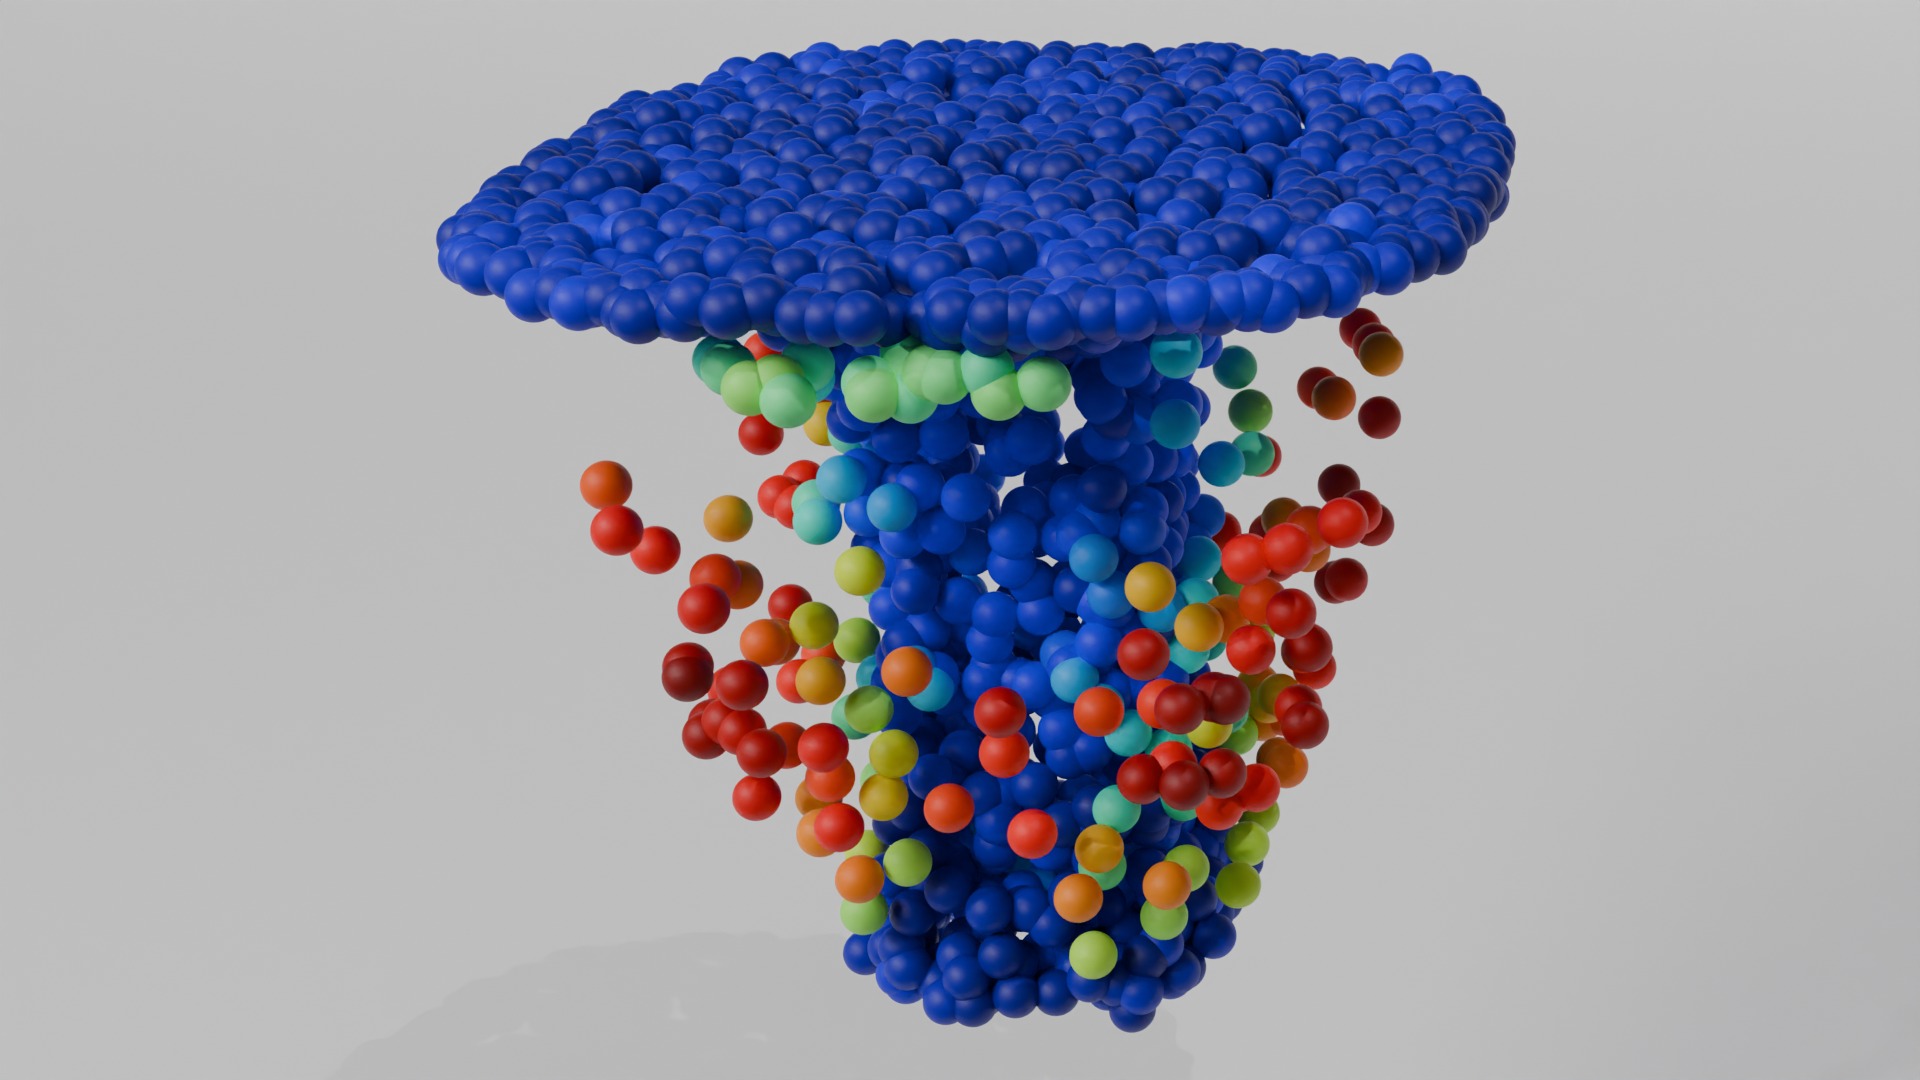
\includegraphics[width=\textwidth]{figures/iml_lin_t3.png}
            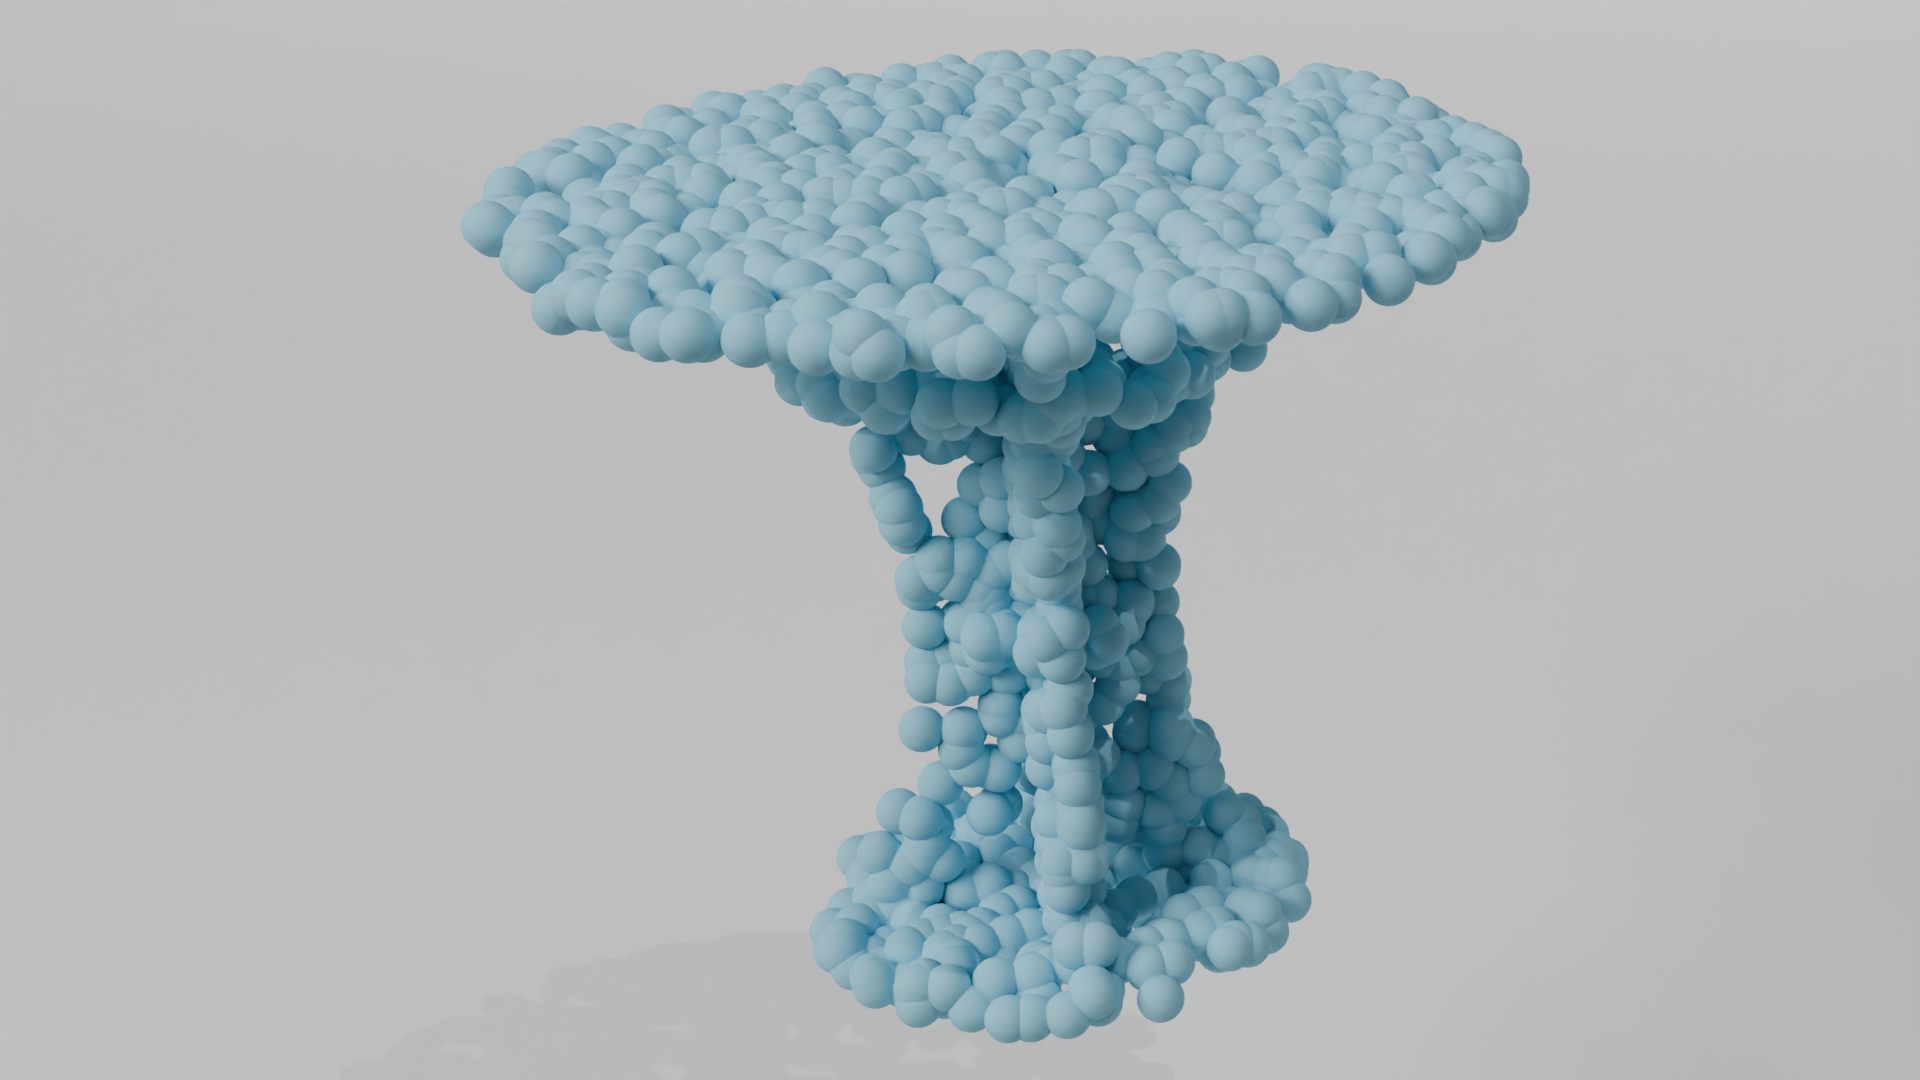
\includegraphics[width=\textwidth]{figures/com_t3.png}
            \caption{Table 3}
          \end{subfigure}
          \caption{Qualitative comparison between different empirical uncertainty quantification methods for point cloud completion on the table subcategory of ShapeNet data. Input refers to the partial point cloud, and GT refers to the ground truth complete cloud. DropCon, Dropout, Ensemble, and Implicit refer to the uncertainty maps output by the DropConnect, dropout, deep ensemble, and implicit generative model-based methods, respectively.}
          \label{fig:table}
        \end{figure}

        \subsubsection{Effect of Number of Generated Samples}
        A comparison between the uncertainty maps produced by different numbers of generated clouds is shown in Figure~\ref{fig:zairplanezz} for a randomly selected example from the airplane subcategory of ShapeNet data. For each input, 5, 10, 25, and 50 different completions were produced for three methods, and uncertainty maps were computed using linear assignment matching between the generated clouds. Ensemble-based methods were ignored due to the computational cost and the memory required to store the models.
        \begin{figure}[htb]
          \centering
          \begin{subfigure}[t]{\dimexpr0.315\textwidth+20pt\relax}
            \makebox[20pt]{\raisebox{30pt}{\rotatebox[origin=c]{90}{\small Input}}}%
            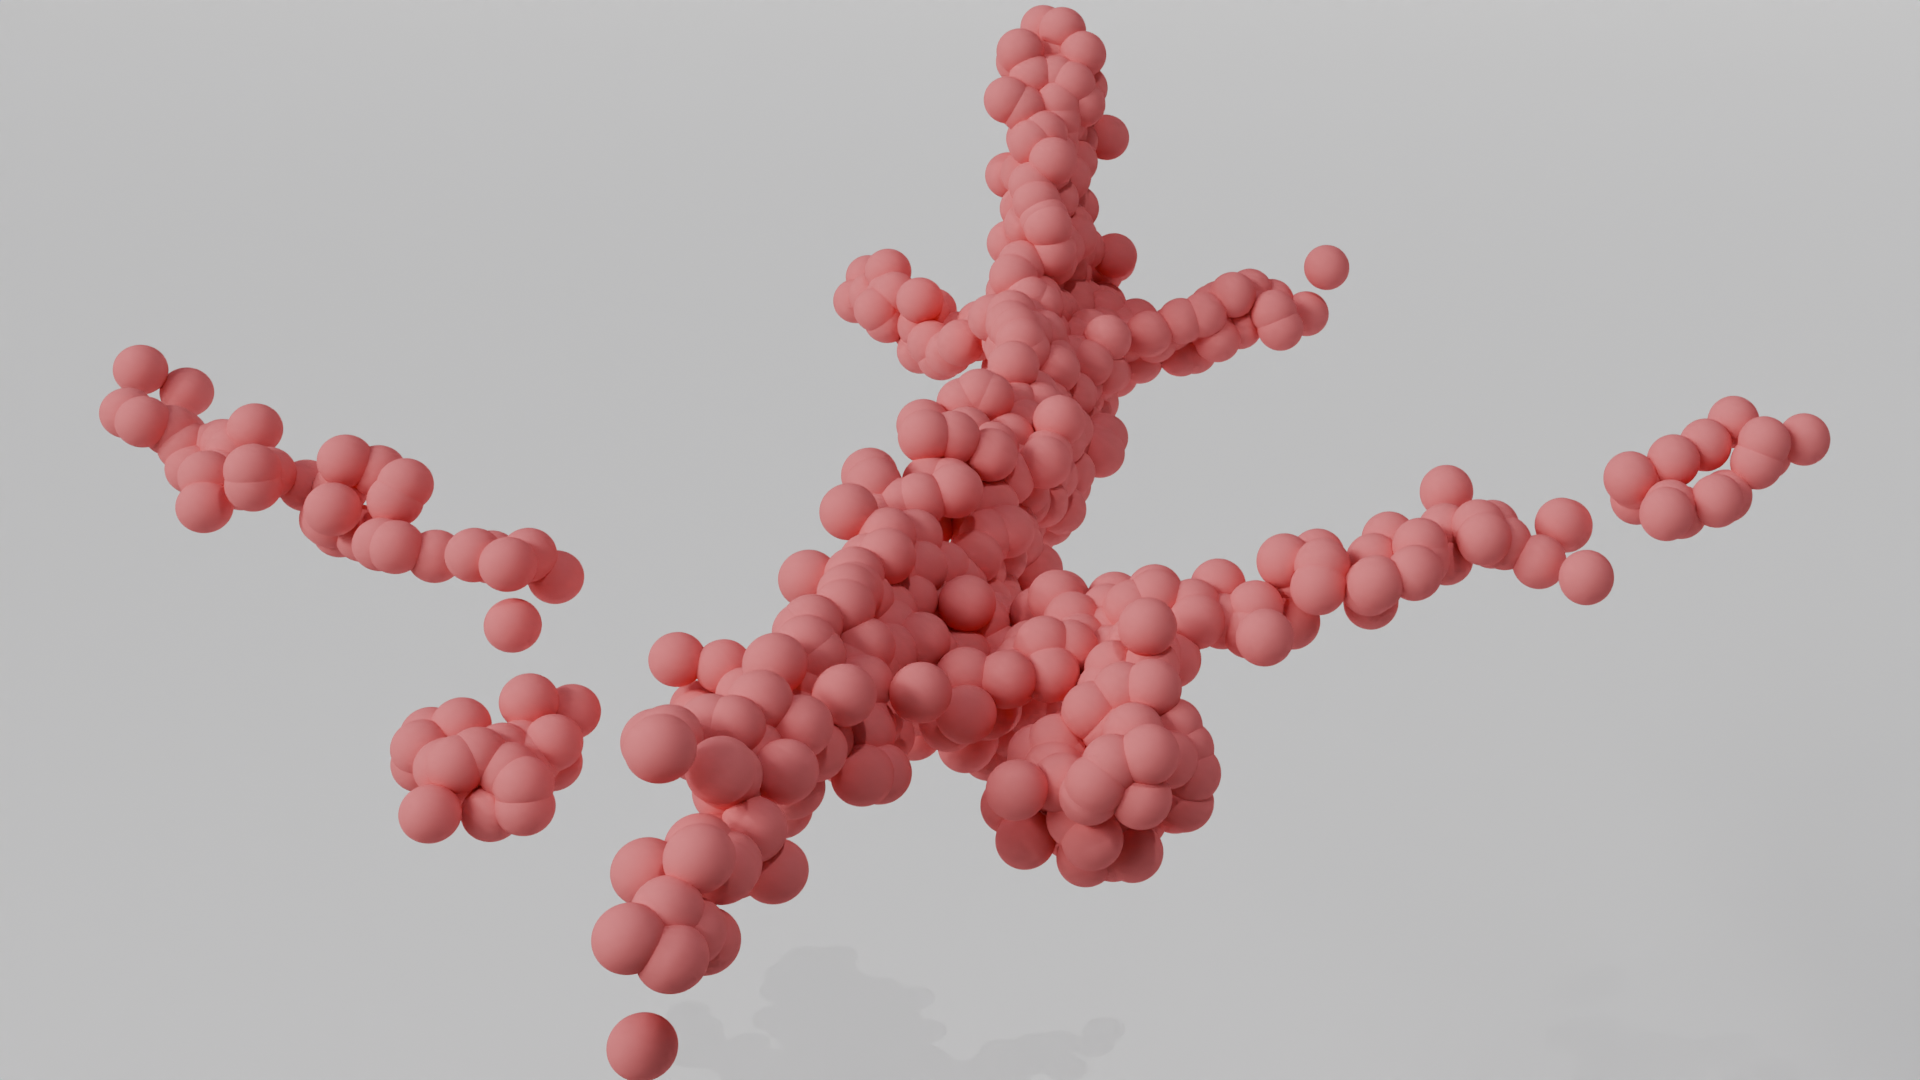
\includegraphics[width=\dimexpr\linewidth-20pt\relax]{figures/part_ap.png}
            \makebox[20pt]{\raisebox{30pt}{\rotatebox[origin=c]{90}{\small $M$=5}}}%
            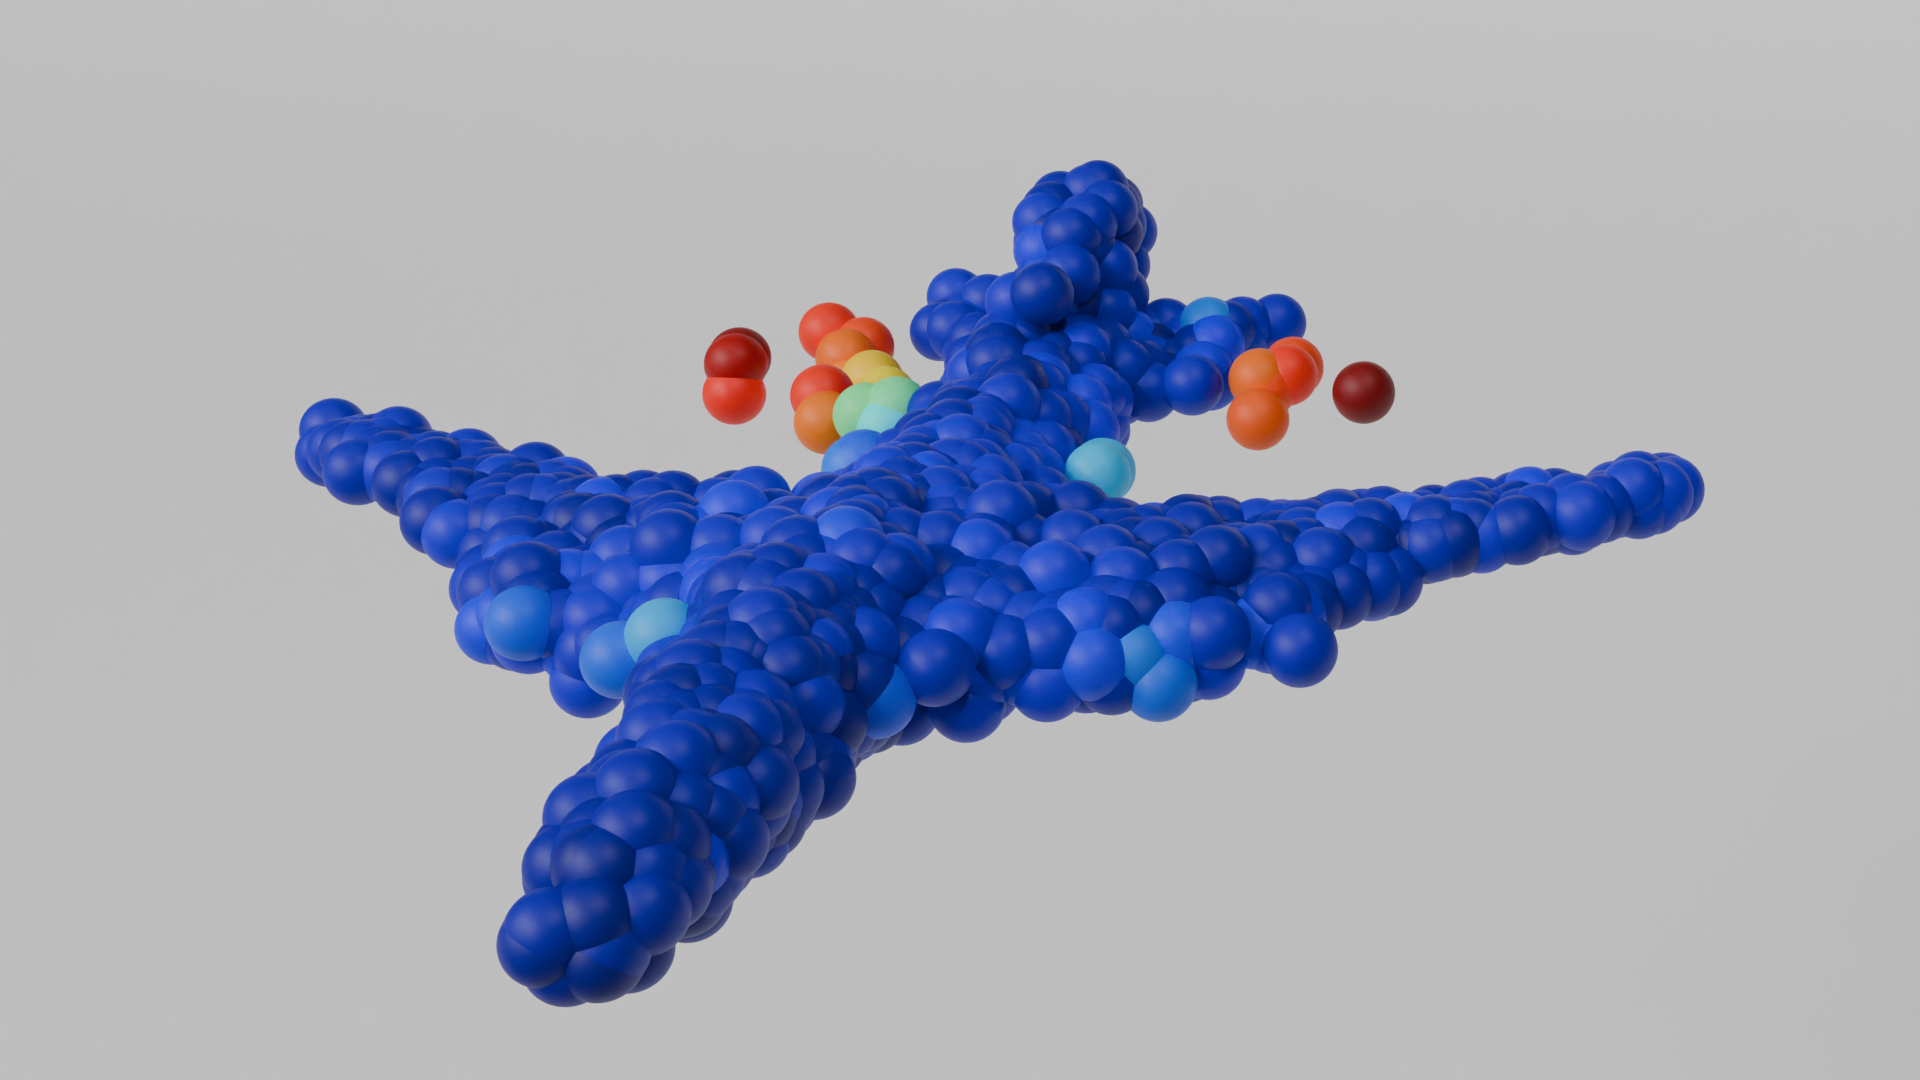
\includegraphics[width=\dimexpr\linewidth-20pt\relax]{figures/5z_ap_mcdc.png}
            \makebox[20pt]{\raisebox{30pt}{\rotatebox[origin=c]{90}{\small $M$=10}}}%
            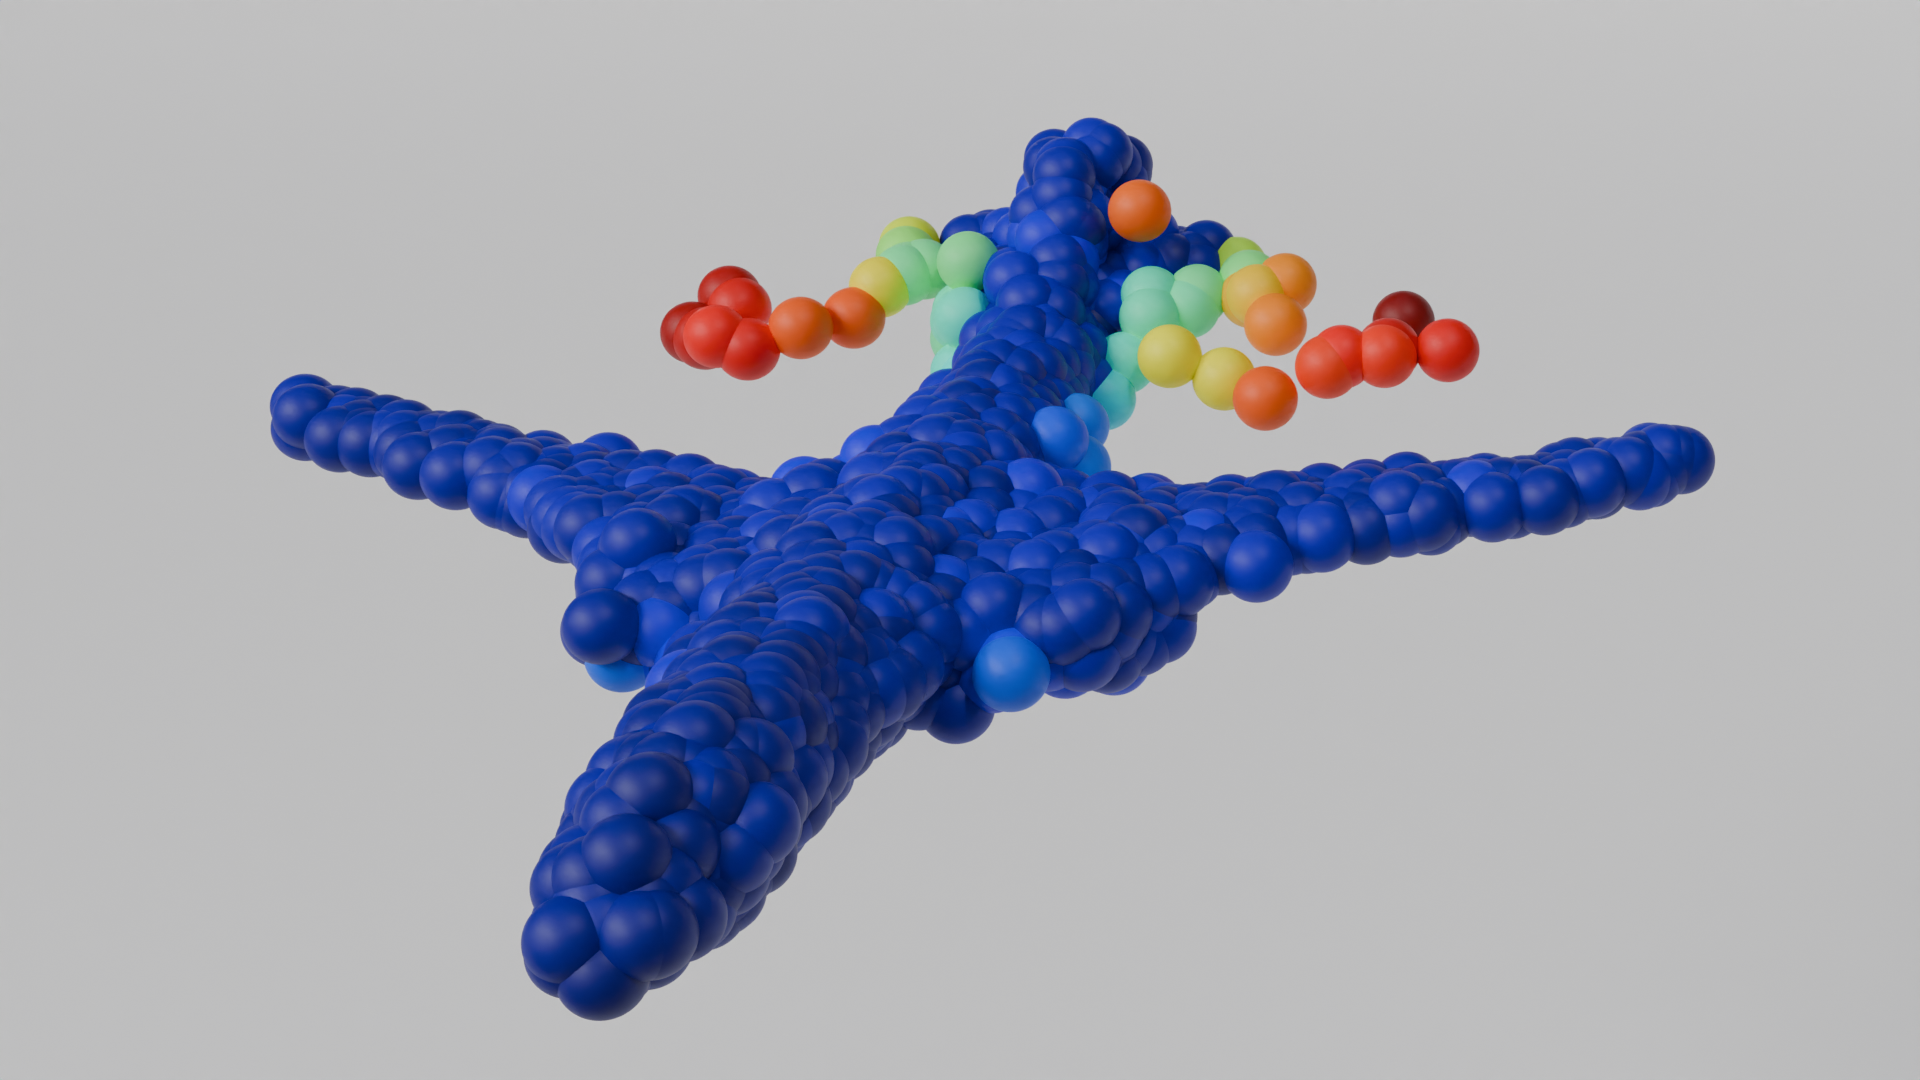
\includegraphics[width=\dimexpr\linewidth-20pt\relax]{figures/10z_ap_mcdc.png}
            \makebox[20pt]{\raisebox{30pt}{\rotatebox[origin=c]{90}{\small $M$=25}}}%
            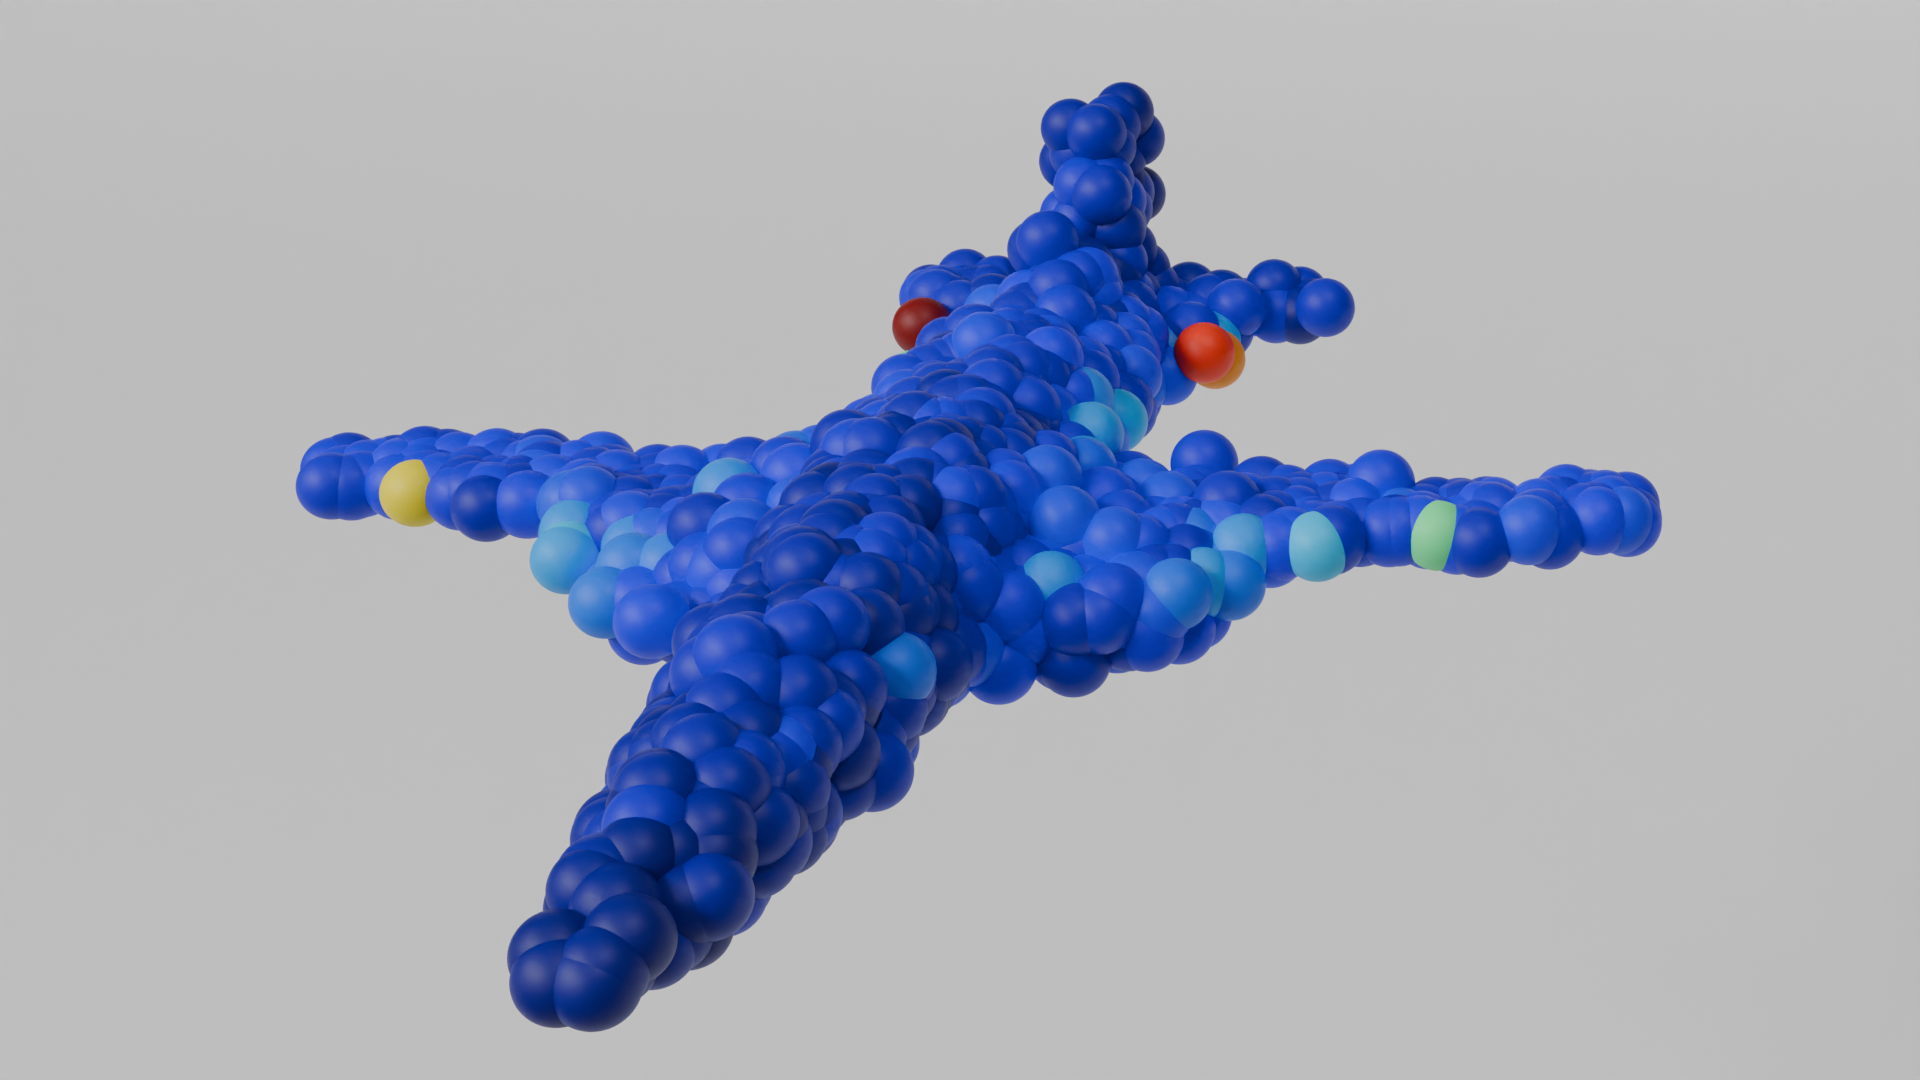
\includegraphics[width=\dimexpr\linewidth-20pt\relax]{figures/25z_ap_mcdc.png}
            \makebox[20pt]{\raisebox{30pt}{\rotatebox[origin=c]{90}{\small $M$=50}}}%
            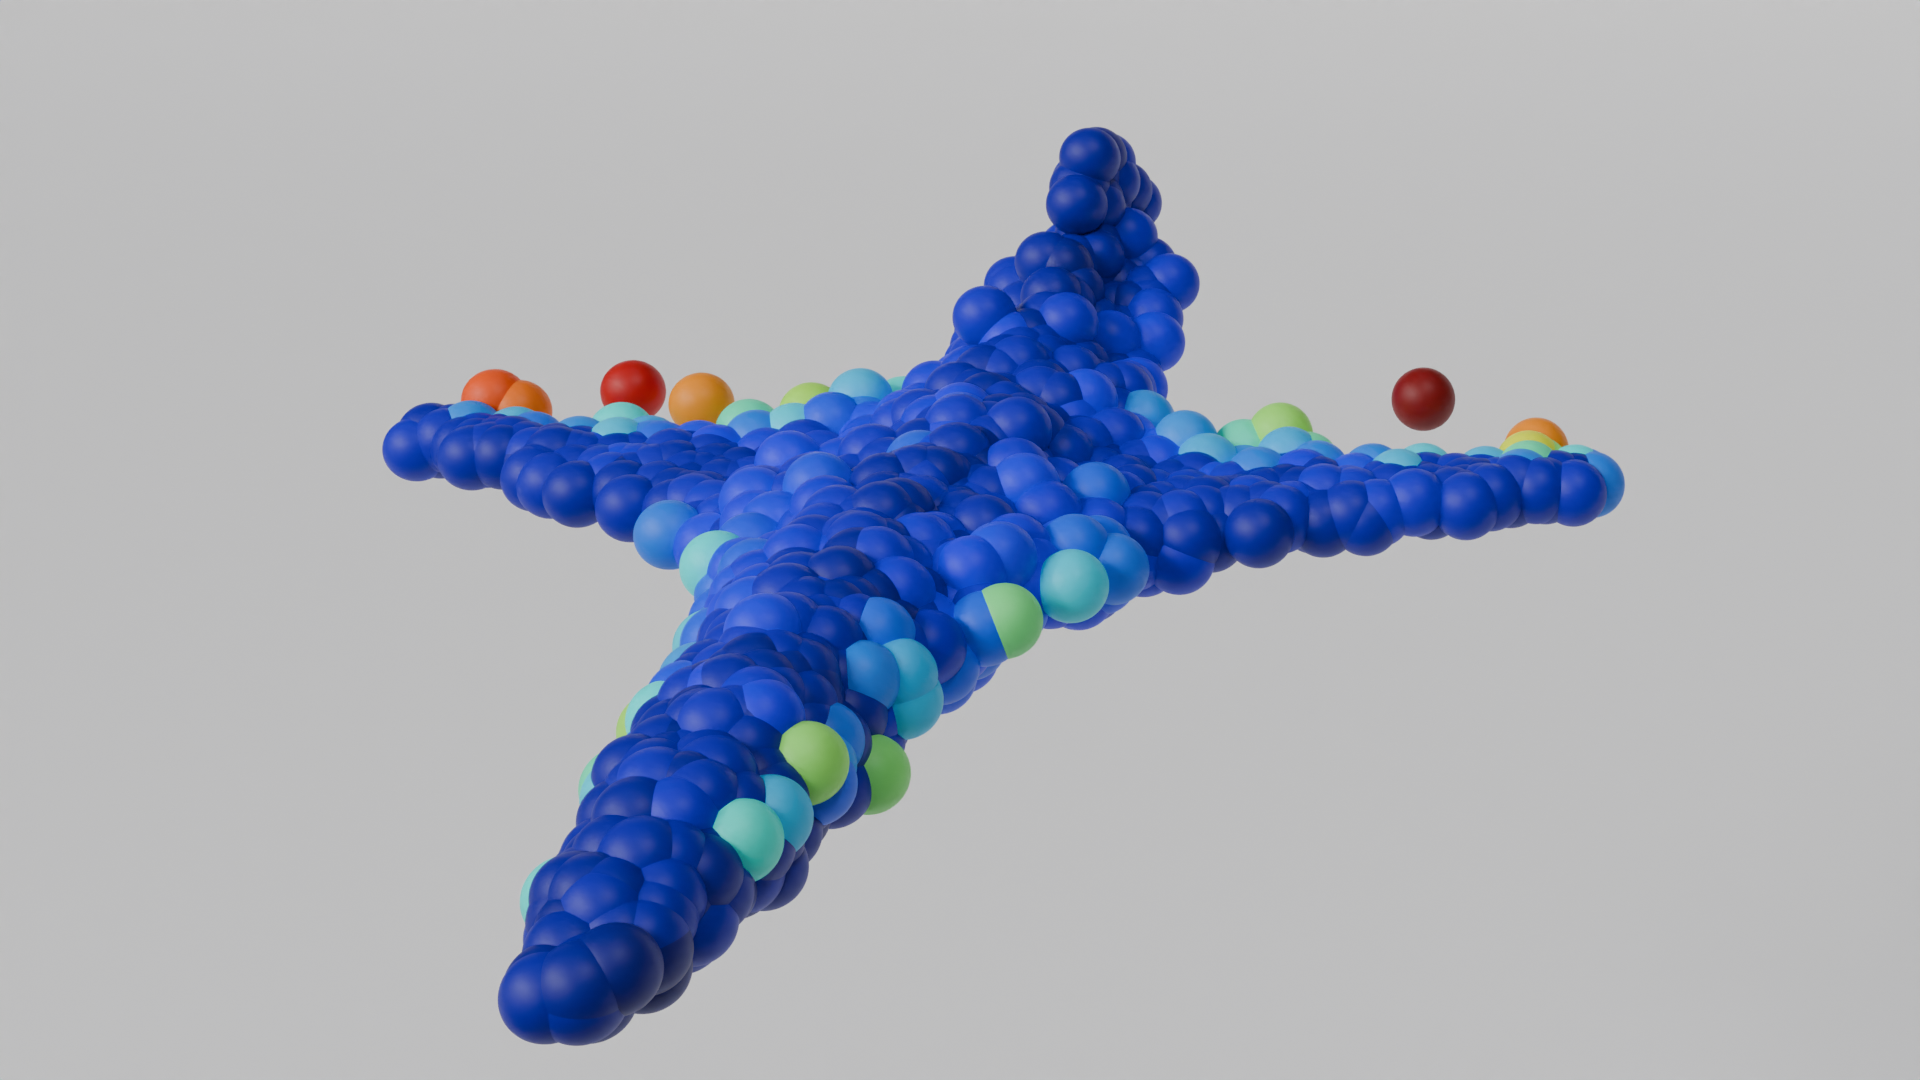
\includegraphics[width=\dimexpr\linewidth-20pt\relax]{figures/50z_ap_mcdc.png}
            \makebox[20pt]{\raisebox{30pt}{\rotatebox[origin=c]{90}{\small GT}}}%
            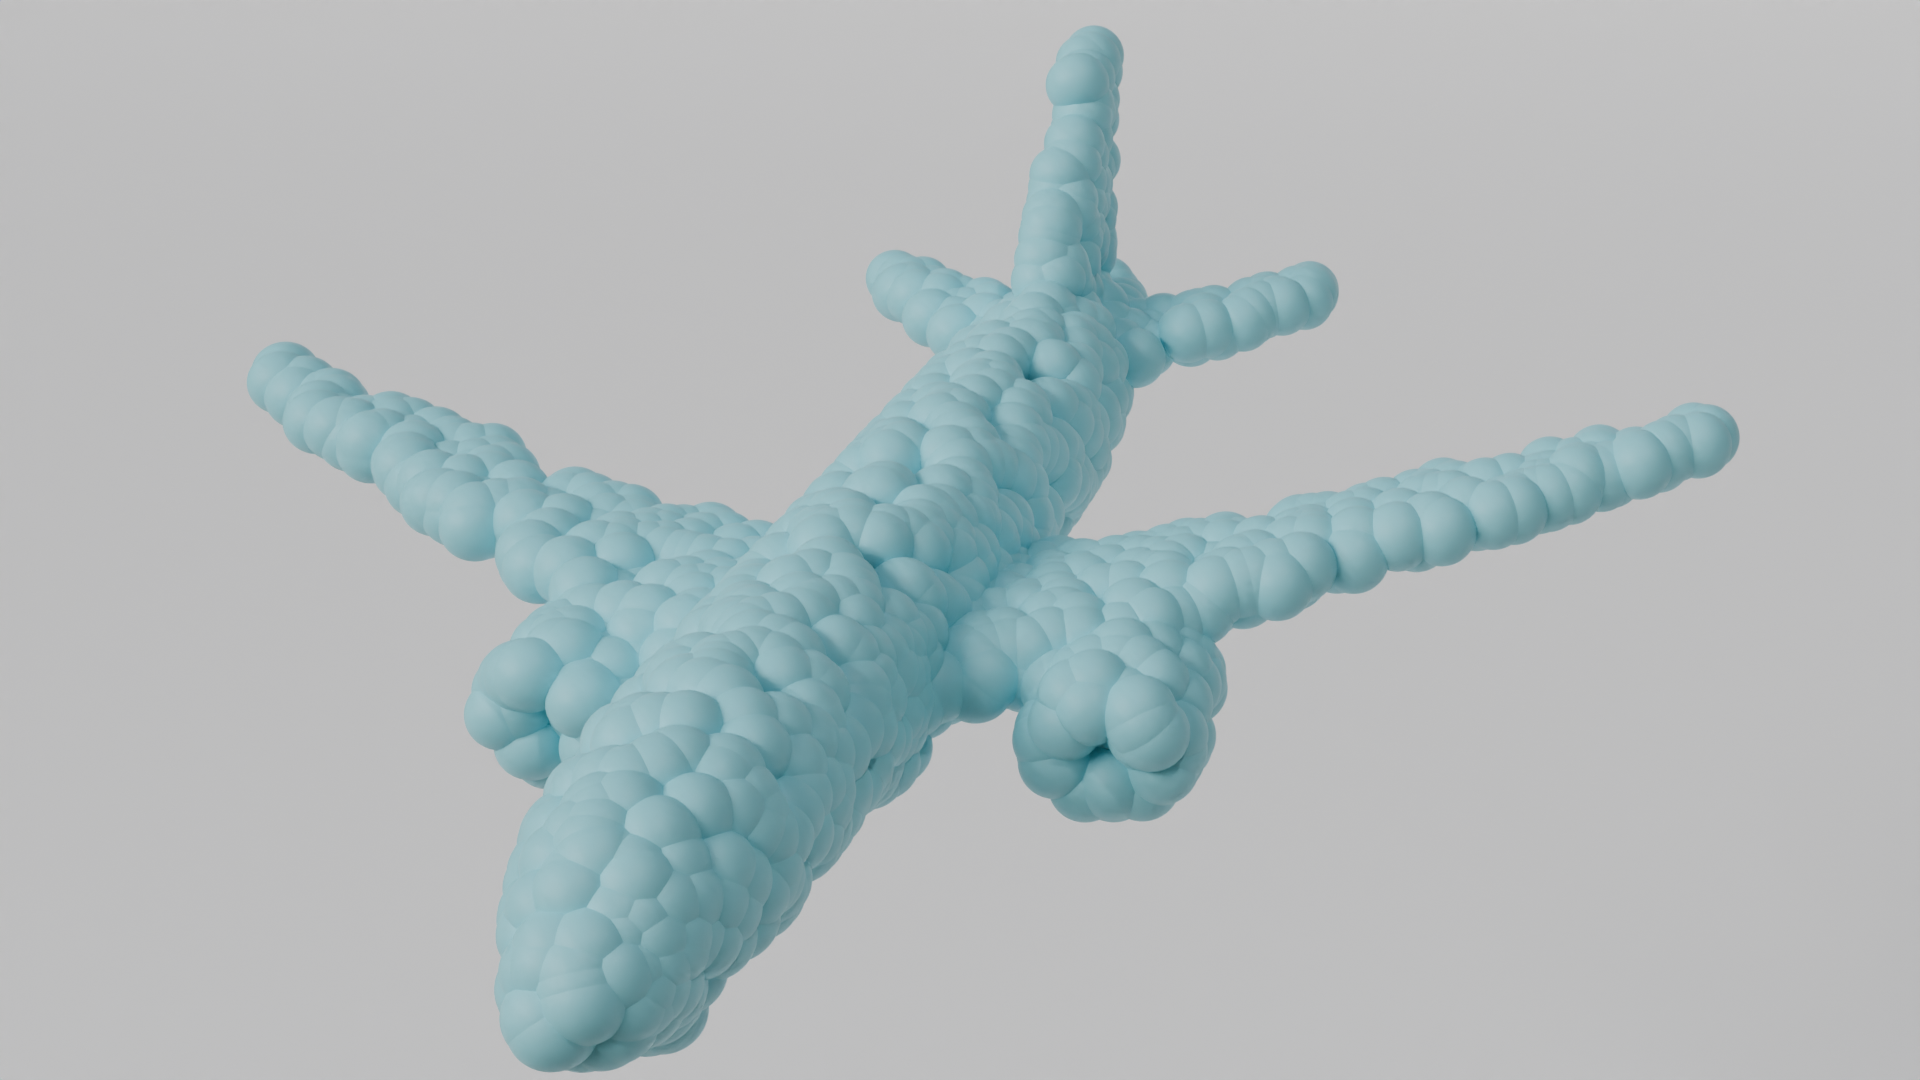
\includegraphics[width=\dimexpr\linewidth-20pt\relax]{figures/comp_ap.png}
            \caption{MC DropConnect}
          \end{subfigure}\hfill
          \begin{subfigure}[t]{0.315\textwidth}
            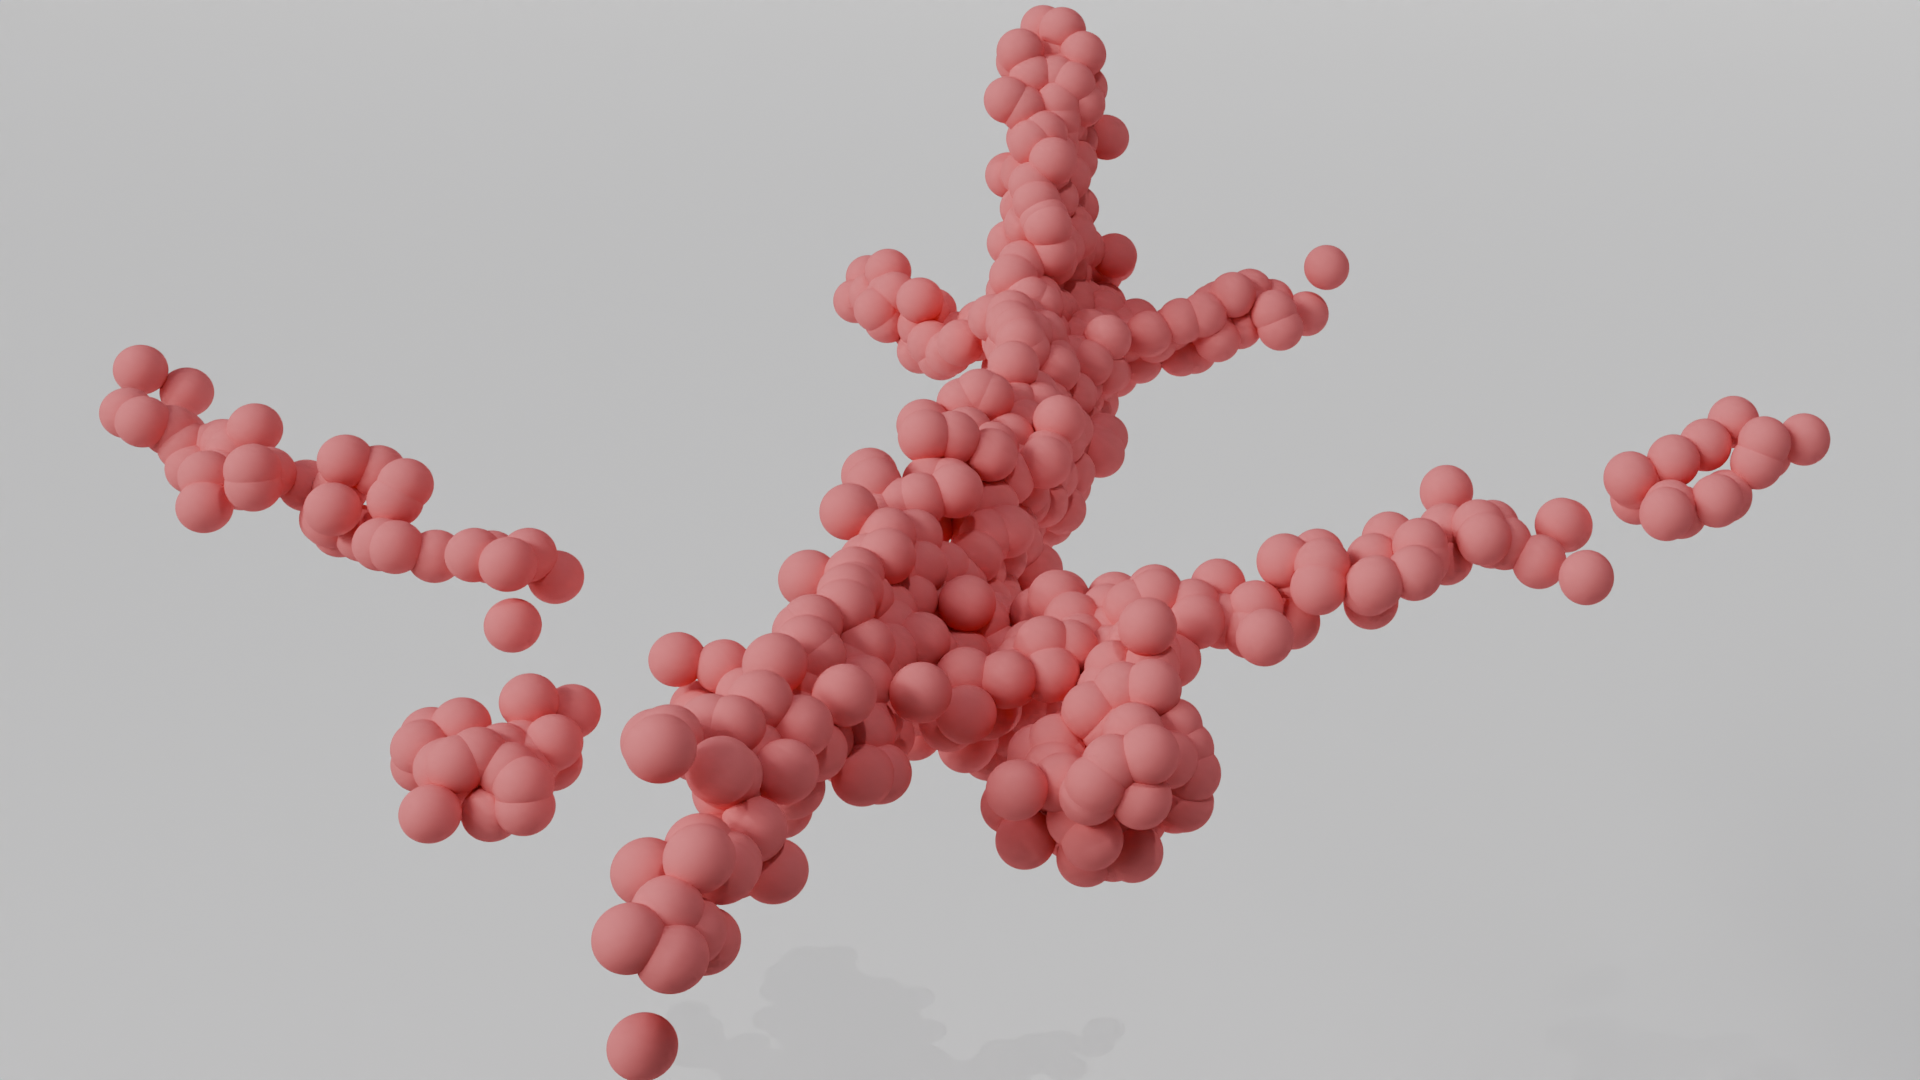
\includegraphics[width=\textwidth]{figures/part_ap.png}
            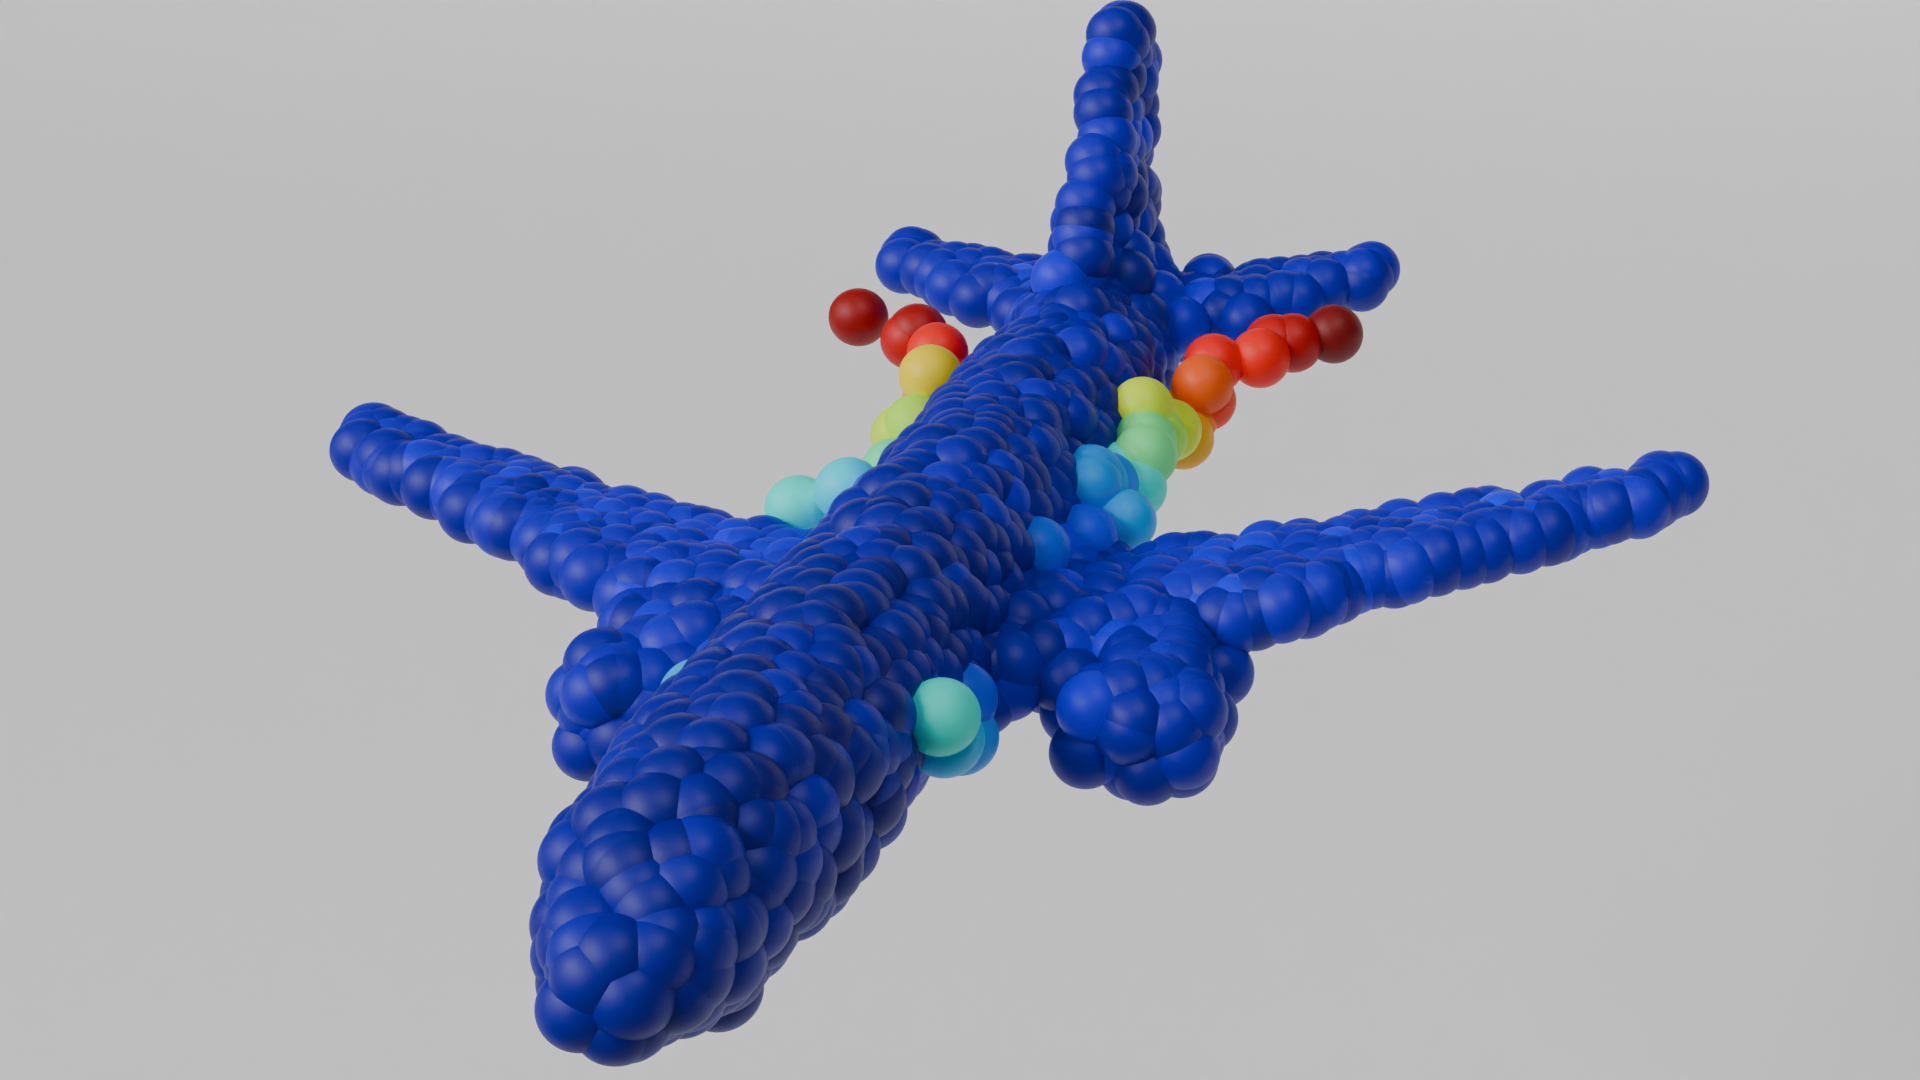
\includegraphics[width=\textwidth]{figures/5z_ap_mcdo.png}
            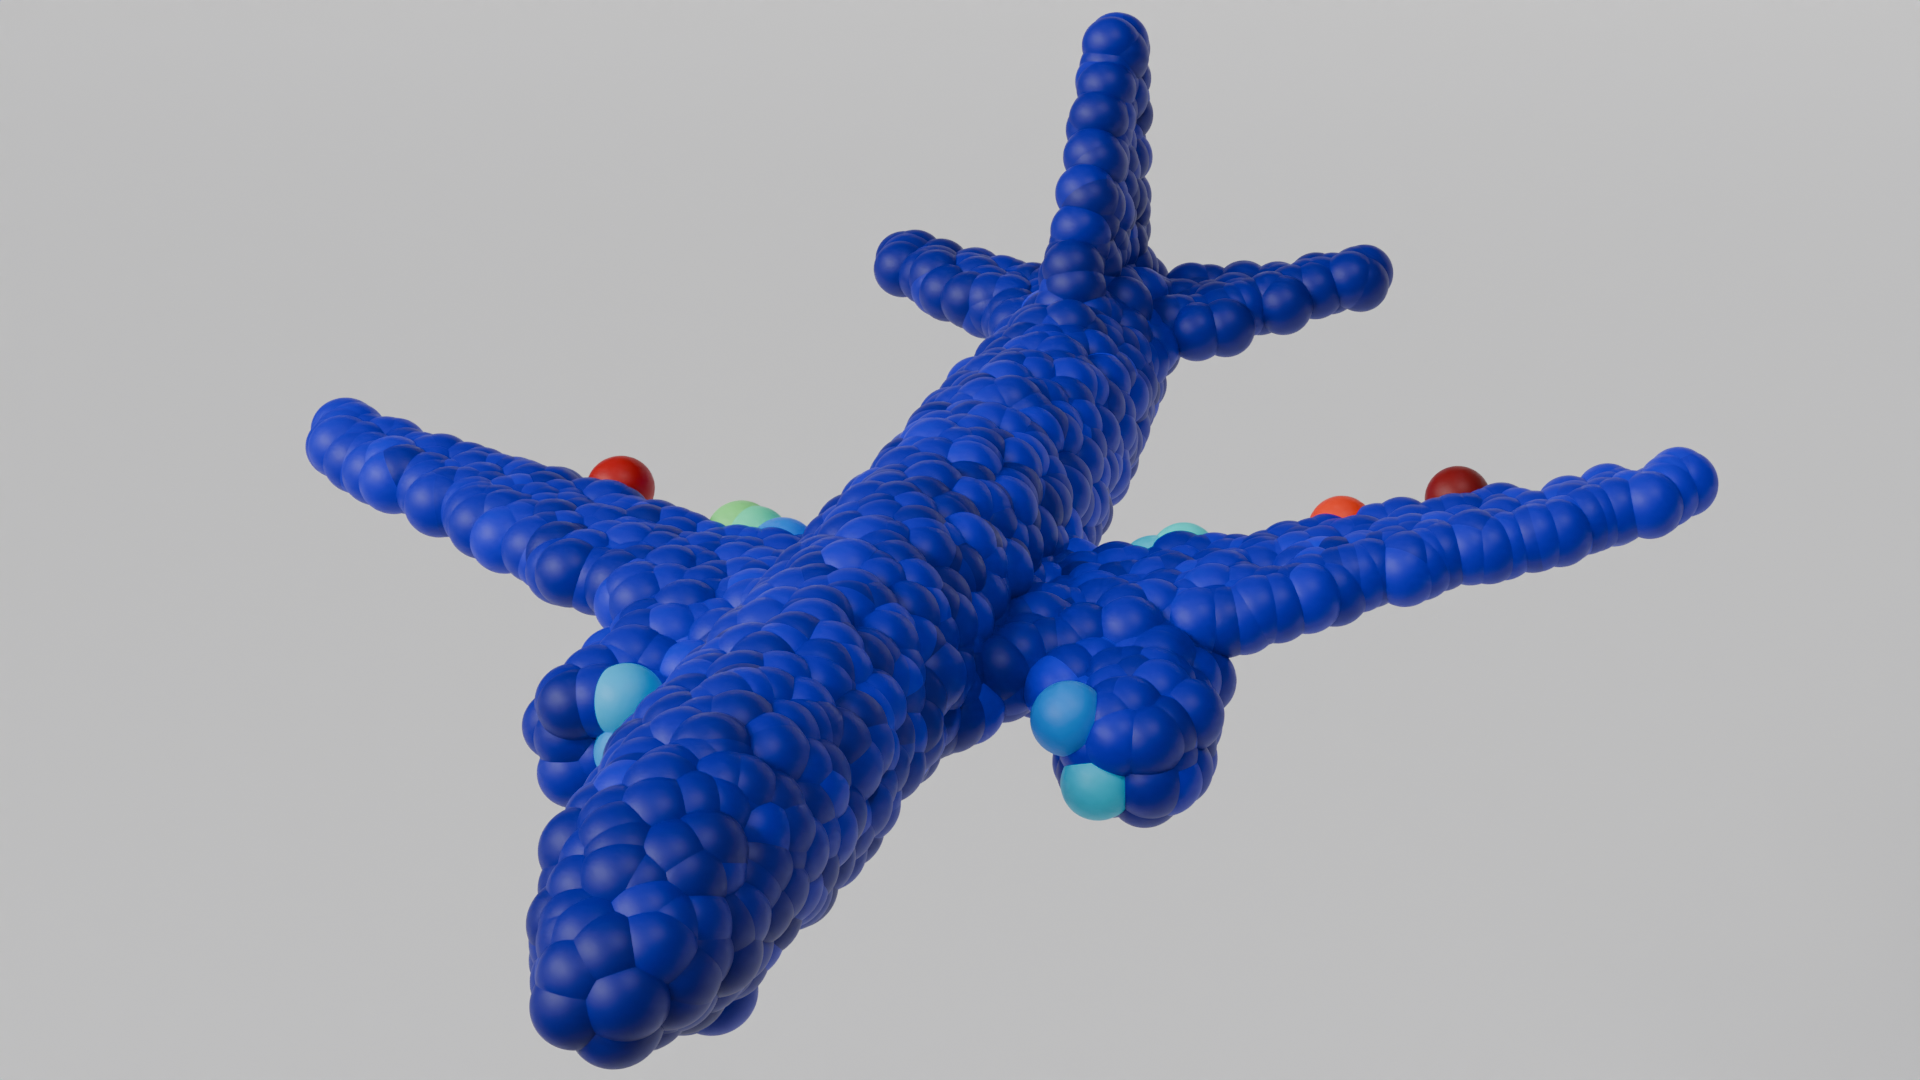
\includegraphics[width=\textwidth]{figures/10z_ap_mcdo.png}
            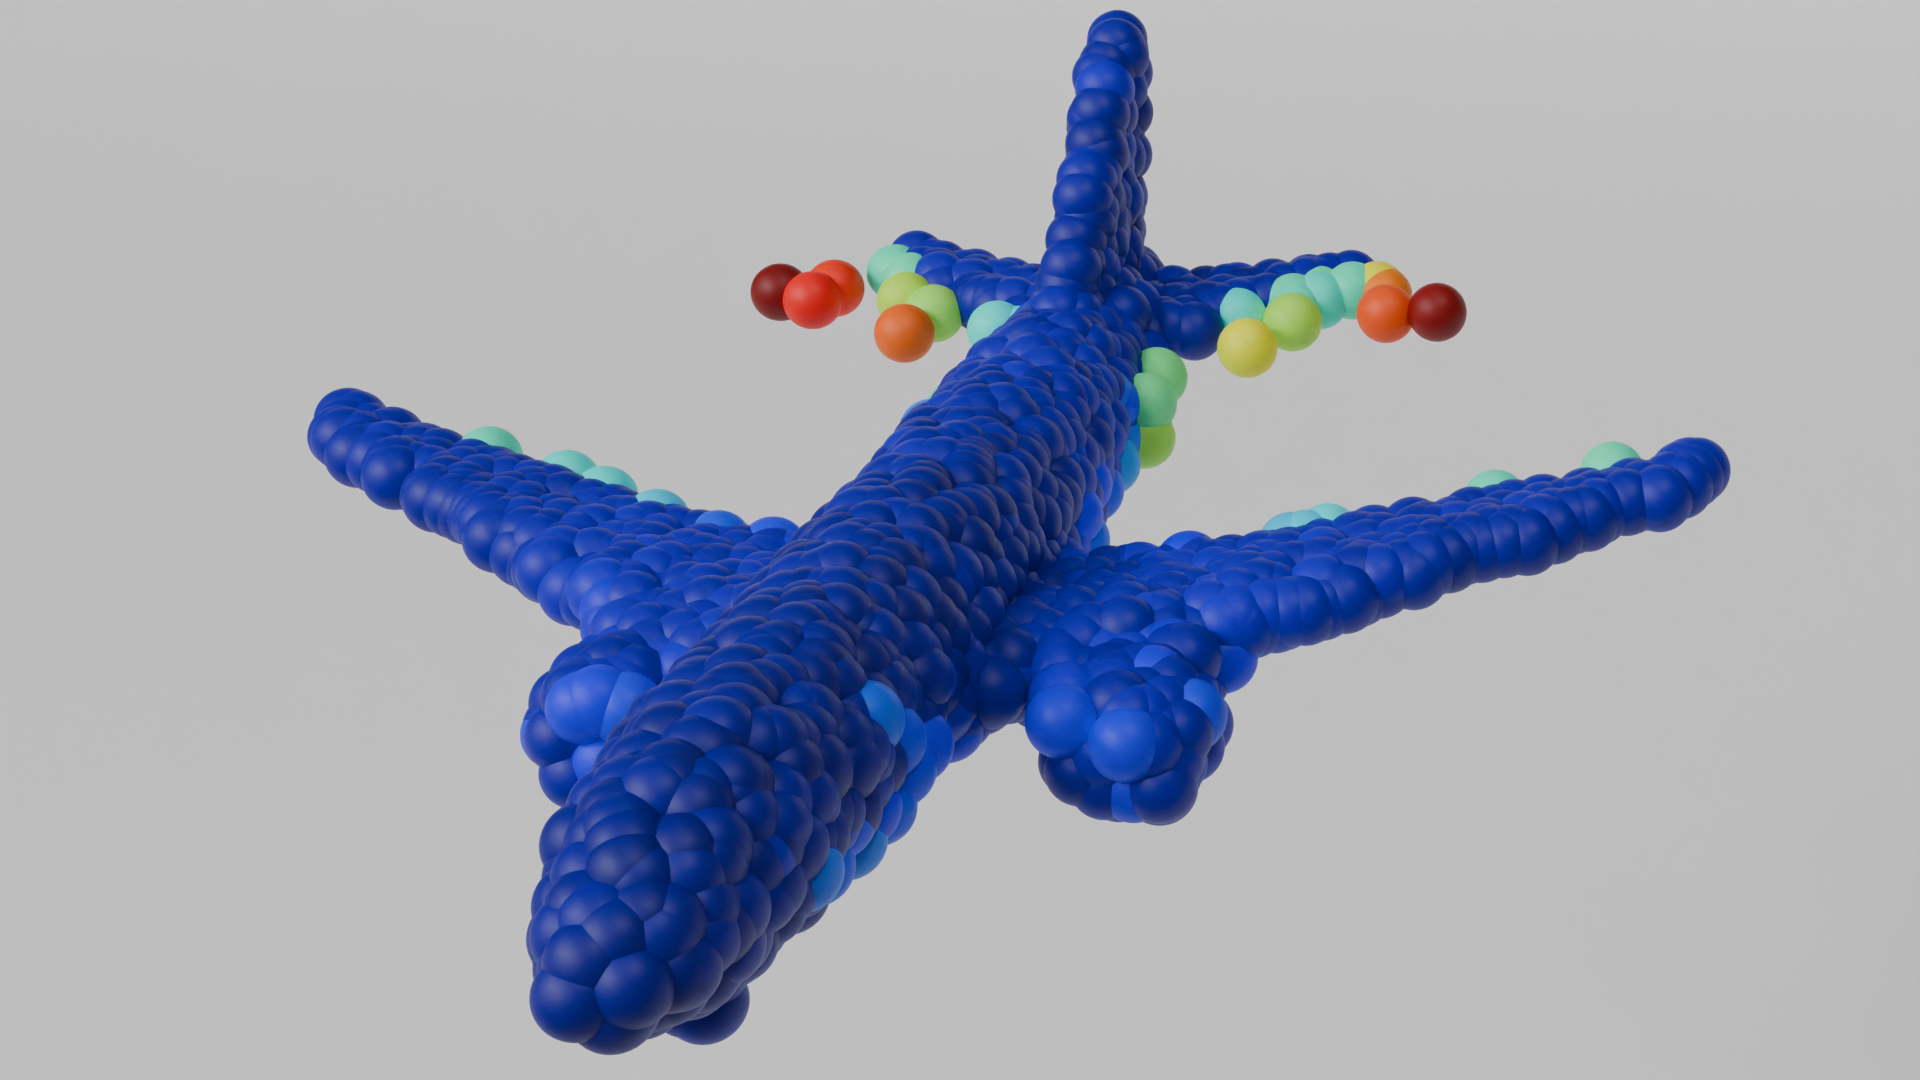
\includegraphics[width=\textwidth]{figures/25z_ap_mcdo.png}
            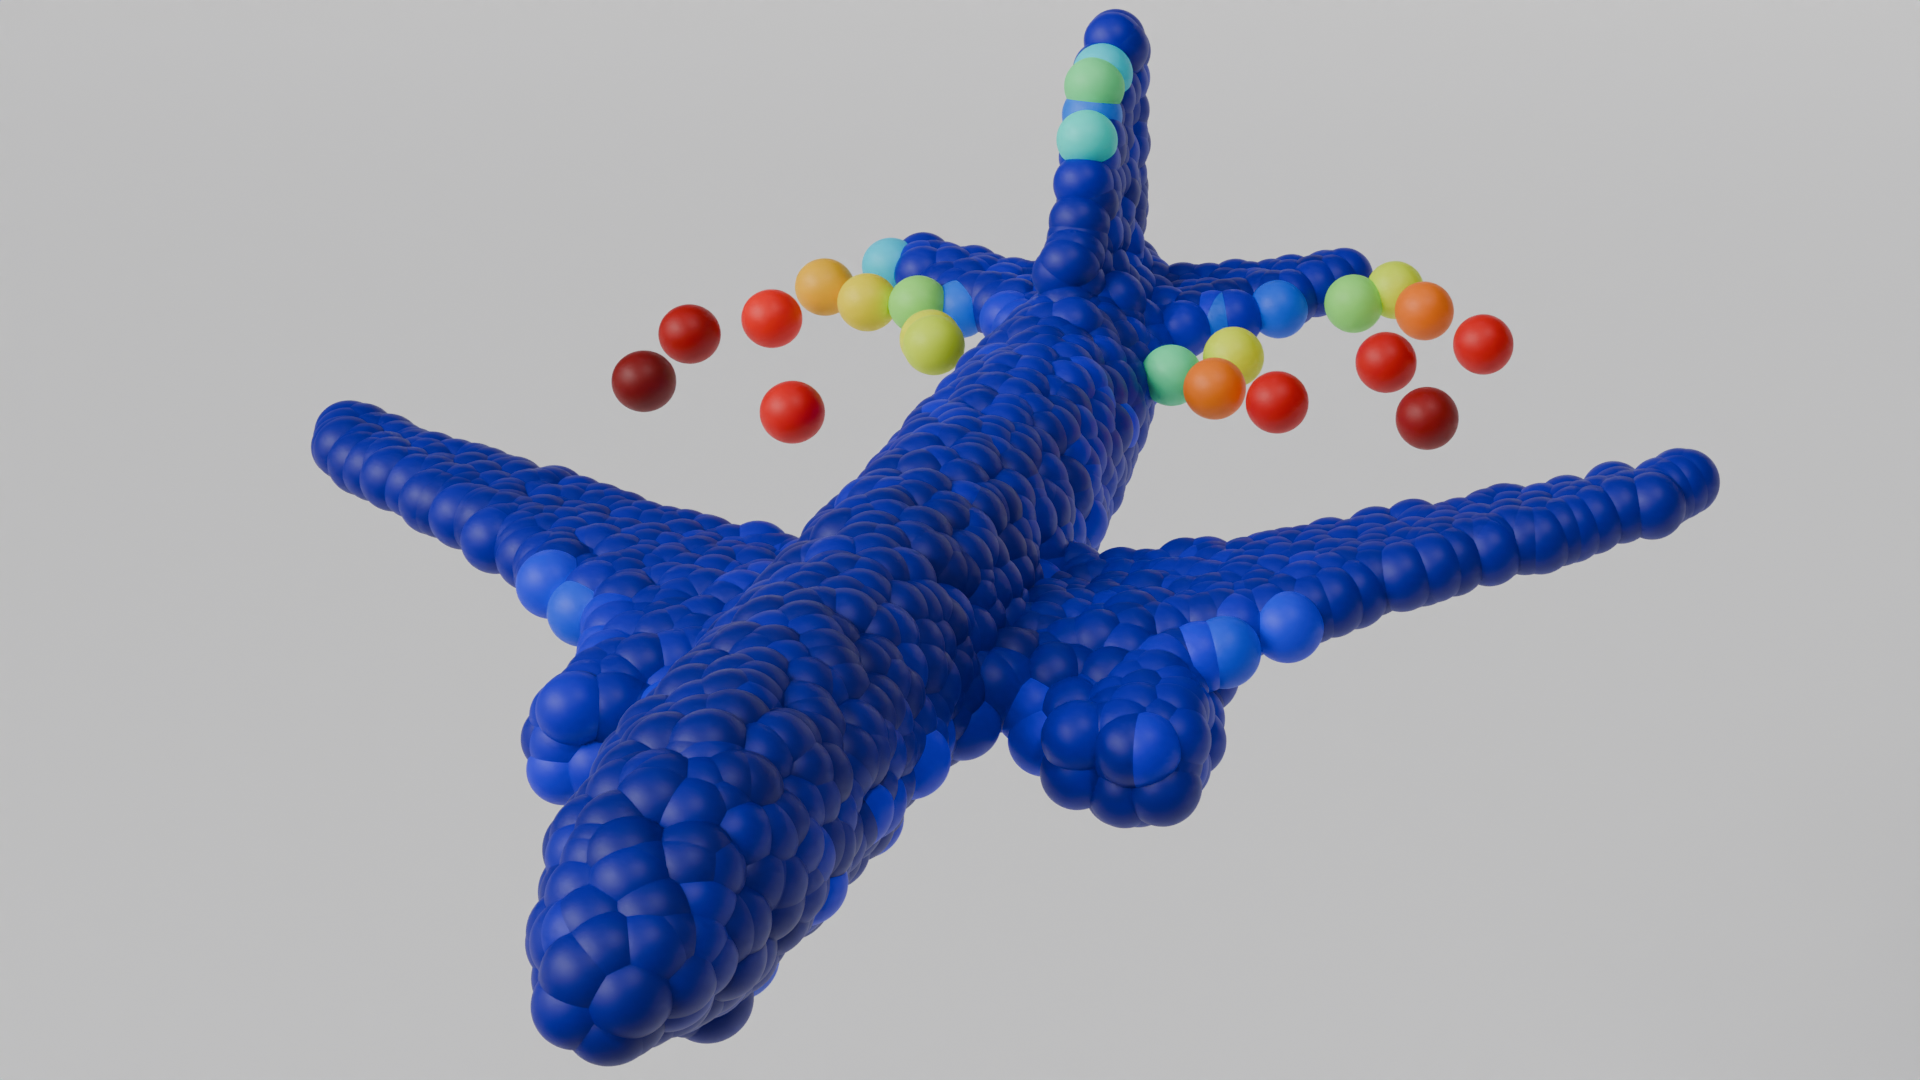
\includegraphics[width=\textwidth]{figures/50z_ap_mcdo.png}
            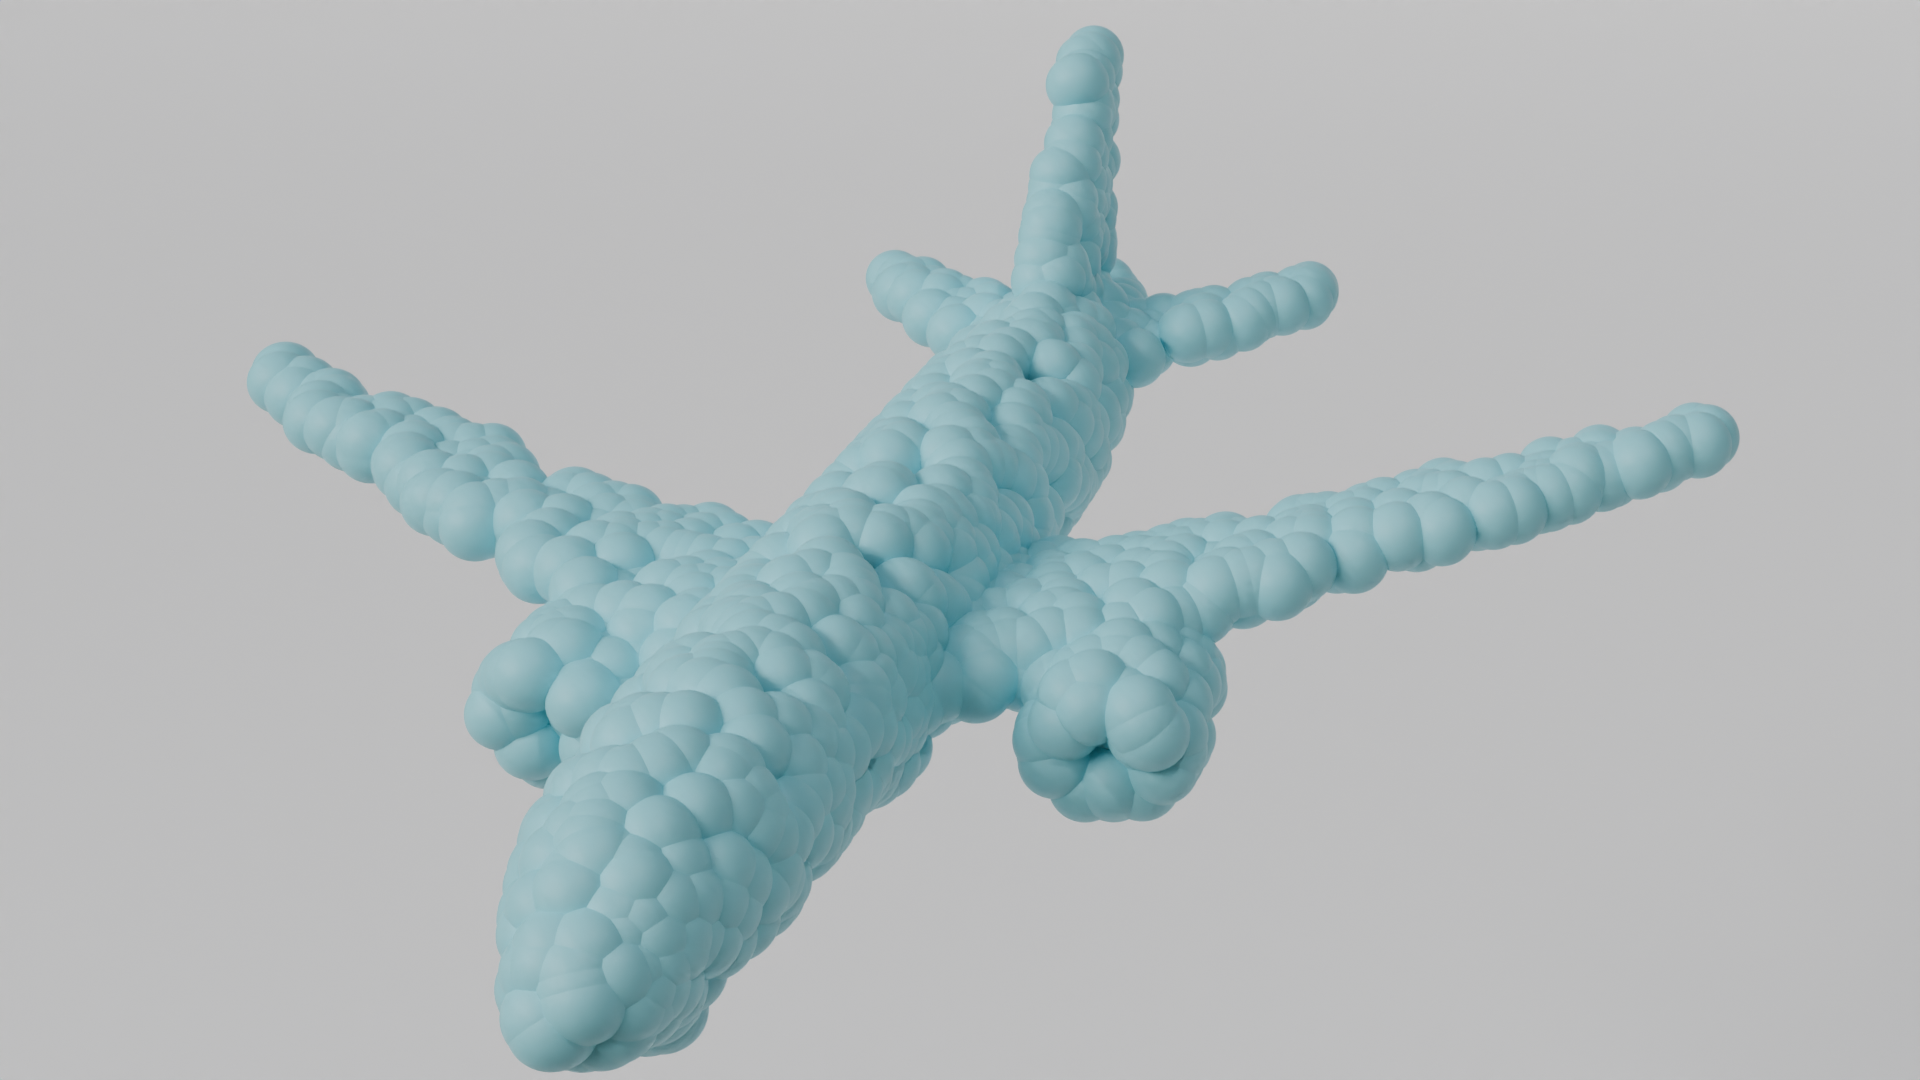
\includegraphics[width=\textwidth]{figures/comp_ap.png}
            \caption{MC Dropout}
          \end{subfigure}\hfill
          \begin{subfigure}[t]{0.315\textwidth}
            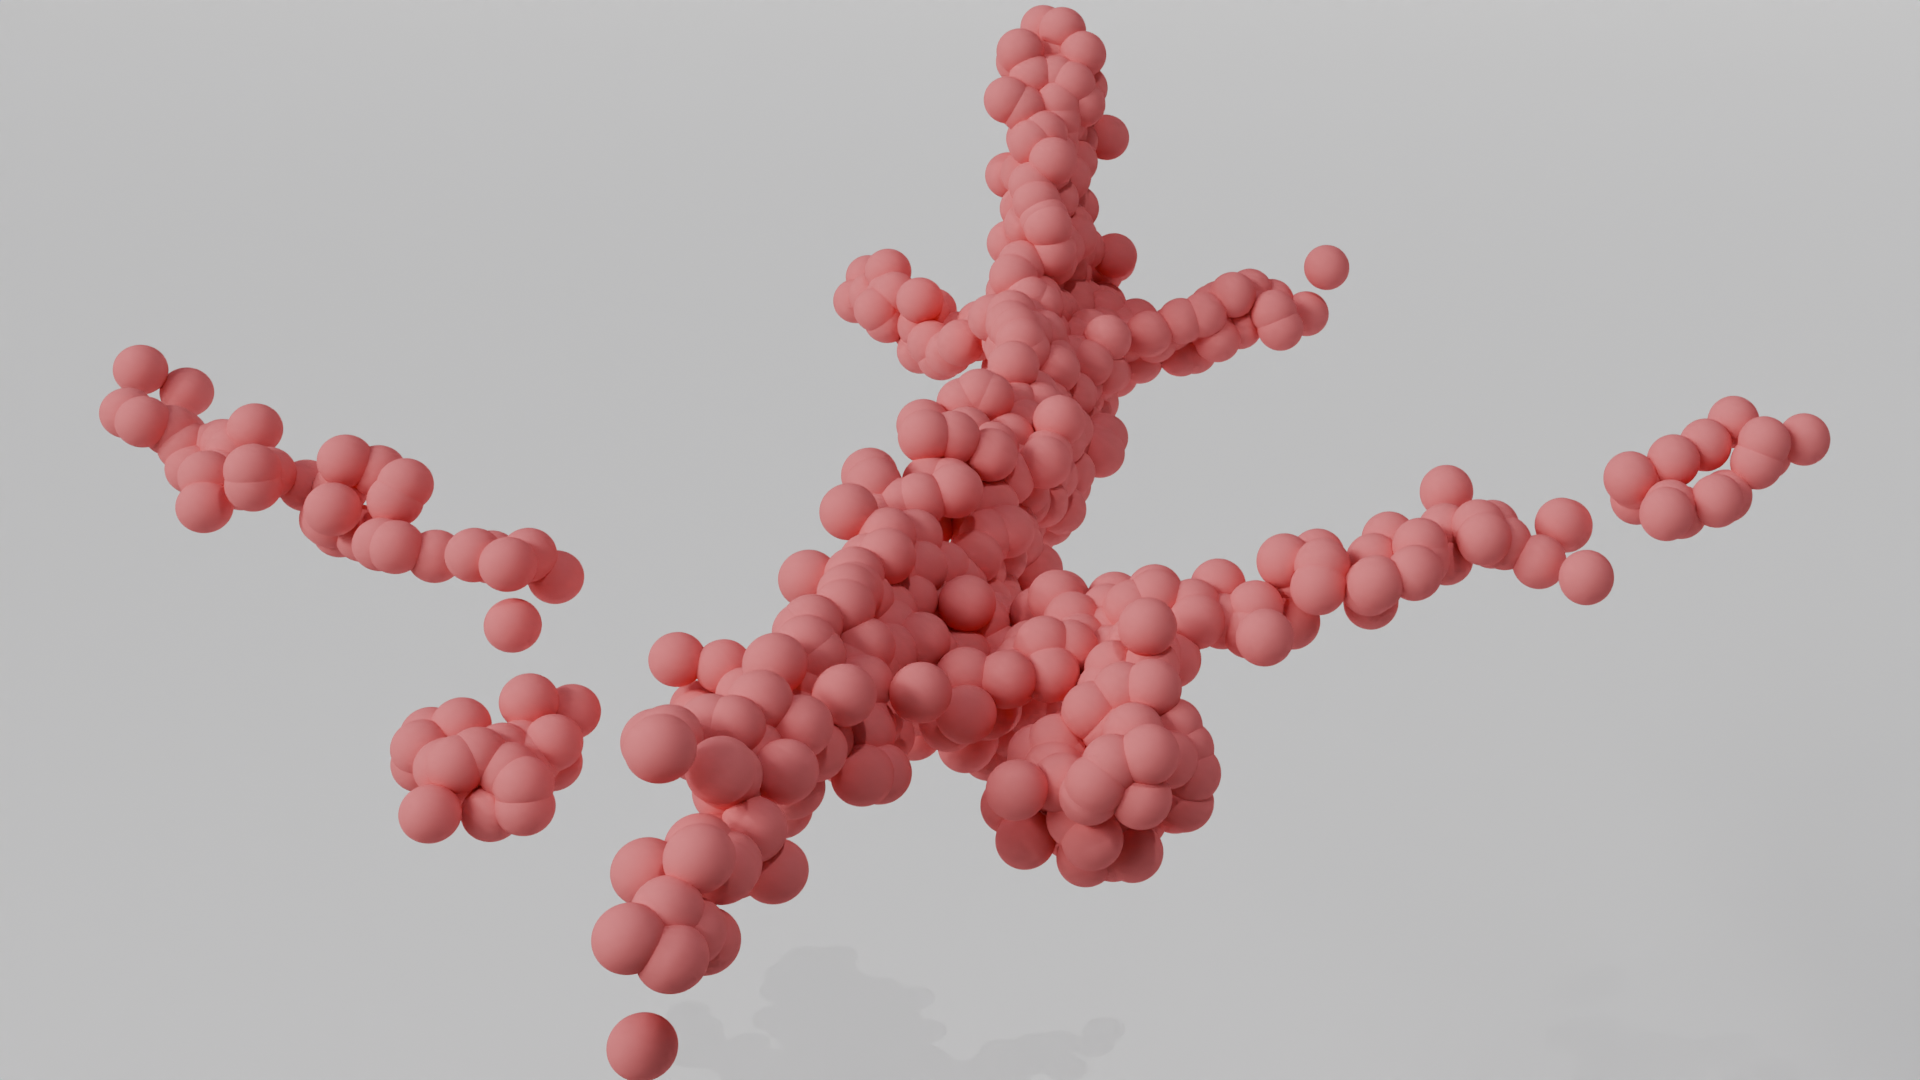
\includegraphics[width=\textwidth]{figures/part_ap.png}
            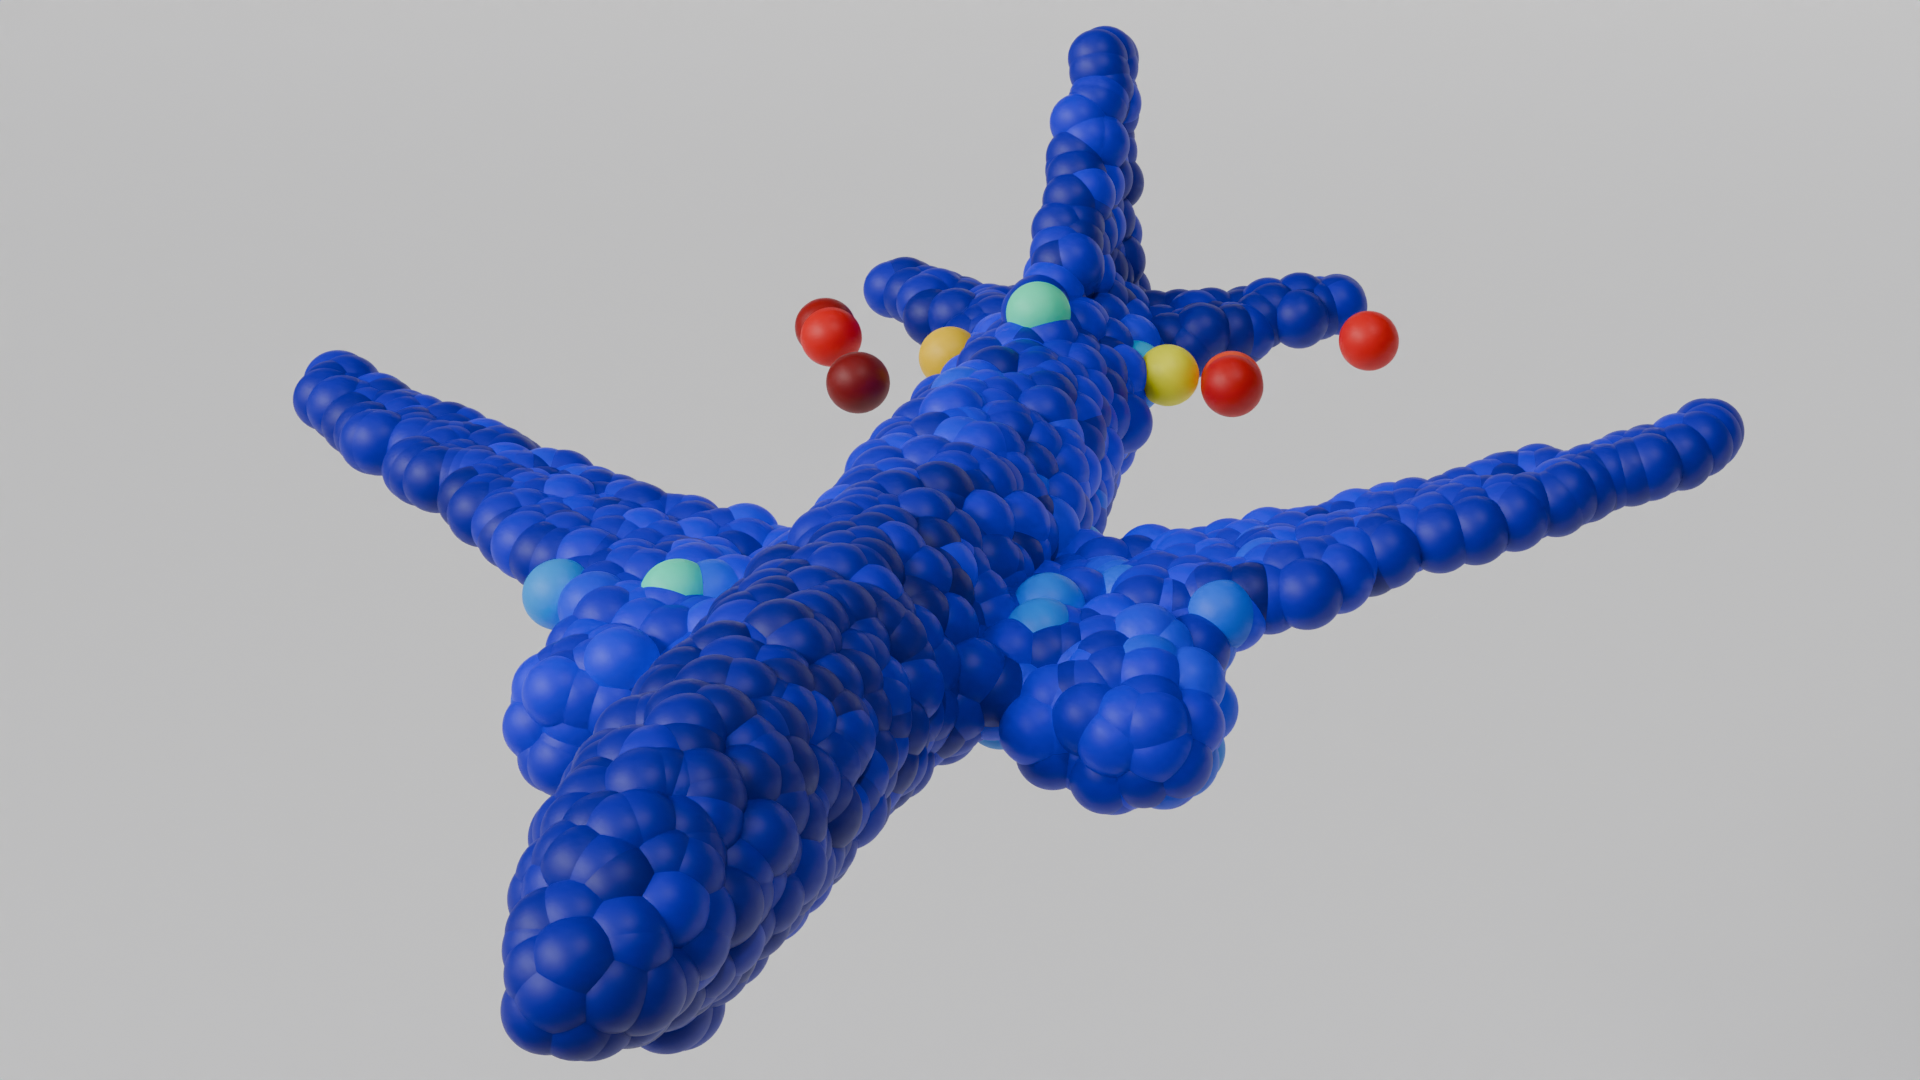
\includegraphics[width=\textwidth]{figures/5z_ap_imle.png}
            \includegraphics[width=\textwidth]{figures/10z_ap_imle.png}
            \includegraphics[width=\textwidth]{figures/25z_ap_imle.png}
            \includegraphics[width=\textwidth]{figures/50z_ap_imle.png}
            \includegraphics[width=\textwidth]{figures/comp_ap.png}
            \caption{Implicit Generation}
          \end{subfigure}
          \caption{Qualitative comparison based on the number of generated clouds used to compute the uncertainty map for different empirical uncertainty quantification methods for point cloud completion on the airplane subcategory of ShapeNet data. Here, $M$ denotes the number of completed clouds generated at inference time. Input refers to the partial point cloud, and GT refers to the ground truth complete cloud.}
          \label{fig:zairplanezz}
        \end{figure}
        \newline

        As seen in Figure~\ref{fig:zairplanezz}, the DropConnect-based model again generated shapes inconsistent with the ground truth. However, across all the models, a common pattern can be observed in the uncertainty map for different sample sizes ($M$). As the numbers of clouds generated were increased, the regions with simpler geometry became less varied. However, the complex geometric regions in the produced clouds became more diverse as more samples were generated. Unfortunately, that resulted in undesired spurious geometries. On the other hand, if too few generated clouds are used to create the uncertainty map, the diversity is not enough. A trade-off can be found for $M$ = 10, which is the value used in all our other experiments, unless stated otherwise.


    \subsection{Quantitative Comparison}
    
        \subsubsection{Uncertainty Map}
        A quantitative comparison between the uncertainty maps produced by different methods described in Section~\ref{euqpcc} is shown in Figure~\ref{fig:normstdairplane} for the airplane subcategory of the ShapeNet dataset. The norms of the standard deviations in the uncertainty map across different test inputs are compared based on specific useful metrics. For each input, 10 different completions were produced, and uncertainty maps were computed using linear assignment matching between the generated clouds. Within each uncertainty map, the standard deviation norms at each point were calculated and stored. In the first column of Figure~\ref{fig:normstdairplane}, histograms of all the norms combined across all test inputs are plotted for the different models implemented. For the second column of Figure~\ref{fig:normstdairplane}, only the maximum standard deviation norm for each test input is collected, and the collection of maximum norms across the test inputs is plotted in histograms for the different models. Finally, for the third column of Figure~\ref{fig:normstdairplane}, the average of standard deviation norms within the uncertainty map for each test input is calculated, and the collection of average norms across the test inputs is plotted in histograms.
        \begin{figure}[htb]
          \centering
          \begin{subfigure}[t]{\dimexpr0.315\textwidth+20pt\relax}
            \makebox[20pt]{\raisebox{60pt}{\rotatebox[origin=c]{90}{\small DropCon}}}%
            \includegraphics[width=\dimexpr\linewidth-20pt\relax]{figures/dropcon/matched_all_std_norms.png}
            \makebox[20pt]{\raisebox{60pt}{\rotatebox[origin=c]{90}{\small Dropout}}}%
            \includegraphics[width=\dimexpr\linewidth-20pt\relax]{figures/dropout/matched_all_std_norms.png}
            \makebox[20pt]{\raisebox{60pt}{\rotatebox[origin=c]{90}{\small Ensemble}}}%
            \includegraphics[width=\dimexpr\linewidth-20pt\relax]{figures/ensemble/matched_all_std_norms.png}
            \makebox[20pt]{\raisebox{60pt}{\rotatebox[origin=c]{90}{\small Implicit}}}%
            \includegraphics[width=\dimexpr\linewidth-20pt\relax]{figures/imle/matched_all_std_norms.png}
            \caption{All norms}\label{fig:normstdairplane1}
          \end{subfigure}\hfill
          \begin{subfigure}[t]{0.315\textwidth}
            \includegraphics[width=\textwidth]{figures/dropcon/matched_max_std_norms.png}
            \includegraphics[width=\textwidth]{figures/dropout/matched_max_std_norms.png}
            \includegraphics[width=\textwidth]{figures/ensemble/matched_max_std_norms.png}
            \includegraphics[width=\textwidth]{figures/imle/matched_max_std_norms.png}
            \caption{Maximum norms}\label{fig:normstdairplane2}
          \end{subfigure}\hfill
          \begin{subfigure}[t]{0.315\textwidth}
            \includegraphics[width=\textwidth]{figures/dropcon/matched_avg_std_norms.png}
            \includegraphics[width=\textwidth]{figures/dropout/matched_avg_std_norms.png}
            \includegraphics[width=\textwidth]{figures/ensemble/matched_avg_std_norms.png}
            \includegraphics[width=\textwidth]{figures/imle/matched_avg_std_norms.png}
            \caption{Average norms}\label{fig:normstdairplane3}
          \end{subfigure}
          \caption{Quantitative comparison based on norms of the standard deviations in the uncertainty maps between different empirical uncertainty quantification methods for point cloud completion on the airplane subcategory of ShapeNet data.}
          \label{fig:normstdairplane}
        \end{figure}
        \newline

        As observed in Figure~\ref{fig:normstdairplane1}, most of the standard deviation norms across all points and all test data remain within the range of 0 to 0.025 for DropConnect-based uncertainty quantification. For both dropout-based and ensemble-based uncertainties, the standard deviation norms mostly lie between 0 and 0.05. In contrast, for implicit generation, the upper range, which contains most norms, extends to 0.1, with a wider tail on the right-hand side of the histogram. These numbers confirm the visual observations presented and discussed in Subsection~\ref{quali}, which show that implicit generation produced the most diverse completions, while DropConnect produced the least diverse completions. The dropout and ensemble models, meanwhile, fall between the implicit generation and DropConnect, with quite similar diversity in their generated complete clouds.
        \\
        When comparing the distribution of maximum standard deviation norms per test data (see Figure~\ref{fig:normstdairplane2}), a similar conclusion can be drawn as above. While the peak of the distribution approximated from the histograms lies around 0.1 for DropConnect, dropout, and ensemble-based methods, the peak is around 0.18 for implicit generation, indicating higher standard deviation across test data.
        \\
        A comparison of the average norms of uncertainty maps per test data (see Figure~\ref{fig:normstdairplane3}) shows an identical pattern to the overall collection of norms. The average norms approximately range from 0.008 to 0.02  for DropConnect, 0.005 to 0.035 for dropout, 0.005 to 0.037 for ensemble, and 0.01 to 0.06 for implicit generation. Altogether, it can be concluded that implicit generative models are capable of producing the most diverse completed shapes from partial inputs out of the methods implemented in this work.
        
        \subsubsection{Shape Approximation Consistency}
        Although the main focus of this work has been on uncertainty quantification for surface reconstruction from partial clouds, it is also essential that the reconstructed surface is consistent with the partial clouds and close to the possible complete shapes. 
        \newline
        
        To quantify the consistency or fidelity of the generated clouds with the partial cloud inputs, the unidirectional Hausdorff distance given by Eq~\ref{fidelity_loss} is computed between the partial cloud and each of the 10 generated clouds. In the first column of Figure~\ref{fig:udhsairplane}, histograms of all the values of unidirectional Hausdorff distance combined across all test inputs from the airplane subcategory of the ShapeNet dataset are plotted for the different models. For the second column, the average of the unidirectional Hausdorff distances between each partial cloud and the corresponding generated complete clouds was computed, and a histogram was plotted for average distances from the individual test inputs.

        \begin{figure}[htb]
          \centering
          \begin{subfigure}[t]{\dimexpr0.36\textwidth+20pt\relax}
            \makebox[20pt]{\raisebox{60pt}{\rotatebox[origin=c]{90}{\small DropCon}}}%
            \includegraphics[width=\dimexpr\linewidth-20pt\relax]{figures/dropcon/all_udhs.png}
            \makebox[20pt]{\raisebox{60pt}{\rotatebox[origin=c]{90}{\small Dropout}}}%
            \includegraphics[width=\dimexpr\linewidth-20pt\relax]{figures/dropout/all_udhs.png}
            \makebox[20pt]{\raisebox{60pt}{\rotatebox[origin=c]{90}{\small Ensemble}}}%
            \includegraphics[width=\dimexpr\linewidth-20pt\relax]{figures/ensemble/all_udhs.png}
            \makebox[20pt]{\raisebox{60pt}{\rotatebox[origin=c]{90}{\small Implicit}}}%
            \includegraphics[width=\dimexpr\linewidth-20pt\relax]{figures/imle/all_udhs.png}
            \caption{All distances}\label{fig:udhsairplane1}
          \end{subfigure}\hfill
          \begin{subfigure}[t]{0.36\textwidth}
            \includegraphics[width=\textwidth]{figures/dropcon/matched_mean_udhs.png}
            \includegraphics[width=\textwidth]{figures/dropout/matched_mean_udhs.png}
            \includegraphics[width=\textwidth]{figures/ensemble/matched_mean_udhs.png}
            \includegraphics[width=\textwidth]{figures/imle/matched_mean_udhs.png}
            \caption{Average distances}\label{fig:udhsairplane2}
          \end{subfigure}
          \caption{Quantitative comparison of fidelity of generated clouds with partial inputs between different empirical uncertainty quantification methods for point cloud completion on the airplane subcategory of ShapeNet data using unidirectional Hausdorff distance.}
          \label{fig:udhsairplane}
        \end{figure}

        As observed in Figure~\label{fig:udhsairplane1}, most of the unidirectional Hausdorff distances are below 1.25 for all methods except DropConnect. For DropConnect, the distribution of the distances is more right-tailed, with most distances below 1.5. The model based on DropConnect was not able to produce complete clouds as consistently as the other models in terms of fidelity with the partial cloud. The histograms of average distances in Figure~\ref{fig:udhsairplane2} show the same kind of distributional patterns. The qualitative comparisons also validated this.
        \newline

        To quantify the approximation quality of the generated clouds with the ground truth complete clouds, the Earth mover's distance given by Eq~\ref{emd_loss} is computed between the complete cloud and each of the 10 generated clouds. In the first column of Figure~\ref{fig:emdsairplane}, histograms of all the values of Earth mover's distance combined across all test data from the airplane subcategory of the ShapeNet dataset are plotted for the different models. For the second column, the average of the Earth mover's distances between each ground truth complete cloud and the corresponding generated clouds was computed, and a histogram was plotted for average distances from the individual test inputs.
        \begin{figure}[htb]
          \centering
          \begin{subfigure}[t]{\dimexpr0.36\textwidth+20pt\relax}
            \makebox[20pt]{\raisebox{60pt}{\rotatebox[origin=c]{90}{\small DropCon}}}%
            \includegraphics[width=\dimexpr\linewidth-20pt\relax]{figures/dropcon/all_emds.png}
            \makebox[20pt]{\raisebox{60pt}{\rotatebox[origin=c]{90}{\small Dropout}}}%
            \includegraphics[width=\dimexpr\linewidth-20pt\relax]{figures/dropout/all_emds.png}
            \makebox[20pt]{\raisebox{60pt}{\rotatebox[origin=c]{90}{\small Ensemble}}}%
            \includegraphics[width=\dimexpr\linewidth-20pt\relax]{figures/ensemble/all_emds.png}
            \makebox[20pt]{\raisebox{60pt}{\rotatebox[origin=c]{90}{\small Implicit}}}%
            \includegraphics[width=\dimexpr\linewidth-20pt\relax]{figures/imle/all_emds.png}
            \caption{All distances}\label{fig:emdsairplane1}
          \end{subfigure}\hfill
          \begin{subfigure}[t]{0.36\textwidth}
            \includegraphics[width=\textwidth]{figures/dropcon/matched_mean_emds.png}
            \includegraphics[width=\textwidth]{figures/dropout/matched_mean_emds.png}
            \includegraphics[width=\textwidth]{figures/ensemble/matched_mean_emds.png}
            \includegraphics[width=\textwidth]{figures/imle/matched_mean_emds.png}
            \caption{Average distances}\label{fig:emdsairplane2}
          \end{subfigure}
          \caption{Quantitative comparison of approximation quality of the generated clouds between different empirical uncertainty quantification methods for point cloud completion on the airplane subcategory of ShapeNet data using Earth mover's distance.}
          \label{fig:emdsairplane}
        \end{figure}

        As observed in Figure~\label{fig:emdsairplane1}, most of the Earth mover's distances are below 0.075 for all methods except DropConnect. For DropConnect, the distribution of the distances is more right-tailed, with most distances below 0.125. The model based on DropConnect was not able to learn to approximate the ground truth complete clouds as well as the other models. The histograms of average distances in Figure~\ref{fig:emdsairplane2} show the same kind of distributional patterns. The qualitative comparisons also validated this.


\section{Evaluation of Implicit Representation-based Empirical Method}
    


\section{Evaluation of Gaussian Process-based Method}